\documentclass{article}
\usepackage{graphicx} 
\graphicspath{{figures/}}
\usepackage{array}
\usepackage{caption}
\usepackage{hyperref}
\usepackage{setspace}
\usepackage{bookmark}
\usepackage{geometry}
\usepackage{listings}
\usepackage{subcaption}
\usepackage[T1]{fontenc}
\usepackage[parfill]{parskip}
\usepackage{lmodern}

\title{MODELLAZIONE E APPRENDIMENTO DI STUDI EPIDEMIOLOGICI CON AGENTI SU GRAFO}
\author{m.stievano1@campus.unimib.it}

\pagenumbering{roman}
\begin{document}
\begin{titlepage}

    \noindent
    \begin{minipage}[t]{0.19\textwidth}
        \vspace{-4mm}{
\includegraphics[scale=1.15]{img/logo_unimib.pdf}}
    \end{minipage}
    \begin{minipage}[t]{0.81\textwidth}
    {
            \setstretch{1.42}
            {\textsc{Università degli Studi di Milano - Bicocca}} \\
            \textbf{Scuola di Scienze} \\
            \textbf{Dipartimento di Informatica, Sistemistica e Comunicazione} \\
            \textbf{Corso di Laurea Magistrale in Informatica} \\
            \par
    }
    \end{minipage}

\vspace{20mm}

\begin{center}
        {\LARGE{
                \setstretch{1.2}
                \textbf{Modellazione e Apprendimento di Studi Epidemiologici con Agenti su Grafo}
                \par
        }}
    \end{center}

    \vspace{60mm}

    \noindent
    {\large \textbf{Relatore:} Prof. Antoniotti Marco} \\

    \noindent
    {\large \textbf{Correlatore:} Prof. }

    \vspace{10mm}

    \begin{flushright}
        {\large \textbf{Relazione della prova finale di:}} \\
        \large{Matteo Stievano} \\
        \large{Matricola 829535}
    \end{flushright}

    \vspace{20mm}
    \begin{center}
        {\large{\bf Anno Accademico 2022-2023}}
    \end{center}

    \restoregeometry

\end{titlepage}

\begin{abstract}
    Lo scopo del presente lavoro è l'analisi e lo studio del comportamento 
    di modelli di simulazione e di intervento nell'ambito della gestione 
    di eventi pandemici, utilizzando il linguaggio di programmazione Julia 
    e alcuni dei suoi framework, tra cui Agents.jl, SciML.ai e Lux.jl.

    Nello specifico, si propone l'adozione del framework Agents.jl come 
    strumento principale per la simulazione di sistemi complessi e 
    l'integrazione di SciML.ai e Lux.jl per lo sviluppo di un controllore 
    in grado di analizzare e interpretare i dati in ingresso. 
    Questo controllore è finalizzato all'apprendimento di strategie di 
    intervento e alla loro applicazione mediante tecniche di machine 
    learning ibrido, come l'utilizzo di Neural ODE.
    
    L'obiettivo è sviluppare un approccio dinamico e ibrido che combini 
    le vantaggiose caratteristiche dei modelli di simulazione e dei 
    modelli matematici. Poiché il problema affrontato è intrinsecamente 
    complesso, è stato modellato come un grafo sociale, 
    cercando di emulare il comportamento di una rete sociale in cui i 
    nodi del grafo rappresentano gli agenti del modello.
    
    Per migliorare le prestazioni e la stabilità del modello, è stato 
    introdotto un sistema di equazioni differenziali ordinarie (ODE) 
    che gestisce e simula l'andamento epidemico di ciascun nodo (agente) 
    del grafo. Il controllore si basa sull'idea di una Neural ODE, 
    che regola in modo autonomo e automatico il livello di contromisure 
    applicate. Tali contromisure sono identificate come una riduzione 
    del numero di individui infetti. Per evitare l'applicazione di 
    contromisure praticamente insostenibili, è stato introdotto un 
    parametro di "felicità", che agisce come una funzione di costo 
    aggiuntiva per il controllore.
\end{abstract}
% se mai volessi scrivere una piccola dedica
\include{./txt/dedica}

% indice dei contenuti
\tableofcontents
\newpage
\listoffigures
\listoftables
\newpage

\pagenumbering{arabic}
% introduzione al testo
\section{Introduzione}

L'impiego di metodologie e tecniche sempre più avanzate è stato oggetto 
di discussione e interesse nella comunità scientifica, in particolare tra 
epidemiologi e medici. Negli ultimi anni, il mondo è diventato notevolmente
interconnesso, aumentando significativamente la probabilità di diffusione 
globale di virus e di conseguenti catastrofi senza precedenti.

La storia umana è segnata da epidemie, ma solo alcune di esse hanno 
lasciato un'impronta duratura nella memoria collettiva a causa delle loro 
conseguenze catastrofiche. Tra queste, alcune delle più note includono la 
peste nera che nel XIV secolo mieté venti milioni di vite in Europa in 
soli sei anni, l'epidemia di tifo durante le crociate e la Seconda 
Guerra Mondiale, l'influenza spagnola che causò 50 milioni di morti tra 
il 1918 e il 1920, e l'epidemia di AIDS, che ha colpito oltre 75 milioni 
di persone e causato 35 milioni di decessi dal 1981.

Oggi, l'influenza stagionale non suscita più lo stesso timore nei 
cittadini dei paesi sviluppati, ma la pandemia di COVID-19, iniziata alla 
fine del 2019, ha condizionato l'umanità per tre anni e continua a farlo, 
causando finora quasi 7 milioni di vittime accertate. Questa pandemia 
rimarrà impressa nella memoria umana poiché ha messo in crisi l'intero 
sistema governativo globale, causando allarmi, panico e, talvolta, 
isteria, come pochi altri eventi sono stati in grado di fare.

Esaminando le statistiche di questa epidemia, i numeri relativi ai decessi 
e agli infetti (quasi 7 milioni di morti e oltre 700 milioni di infetti) 
da soli sono sufficienti a preoccupare qualsiasi lettore. Tuttavia, ci 
sono altri dati meno evidenti che forniscono informazioni altrettanto 
inquietanti, come l'impatto economico globale e il concetto di 
"poverty trap", un circolo vizioso in cui la povertà e le malattie 
perpetuano un ciclo di bassa salute e crescente povertà.

Questi sono solo alcuni dei problemi che possono emergere durante una 
pandemia globale come quella del COVID-19, e quindi la comunità 
scientifica, in particolare gli epidemiologi, cerca costantemente 
soluzioni più efficaci ed accurate per prevenire, contenere e gestire 
eventi di questo genere.

L'epidemiologia è una disciplina relativamente giovane che si è evoluta 
per affrontare emergenze sanitarie. La sua definizione originale risale 
al 1978, ma nel corso del tempo è cresciuta e si è adattata alle esigenze 
della società. Attualmente, l'epidemiologia è definita come lo studio 
della distribuzione e dei determinanti delle condizioni o eventi legati 
alla salute in una specifica popolazione, con l'applicazione di questo 
studio al controllo dei problemi di salute.

Uno strumento ampiamente utilizzato in epidemiologia è la simulazione 
tramite software, che si basa su modelli matematici per trarre conclusioni 
sui sistemi analizzati. Questi sistemi, spesso definiti complessi, 
coinvolgono molteplici componenti che interagiscono tra loro e possono 
essere descritti mediante modelli matematici.

I primi modelli epidemiologici erano compartimentali, basati su gruppi di 
individui separati che interagivano tra loro e potevano essere descritti 
mediante equazioni differenziali ordinarie (ODE). Uno dei modelli più noti 
è il modello Suscettibile-Infetto-Ricoverato (SIR) sviluppato da 
Kermack e McKendrick nel 1927. Successivamente, sono emersi i modelli ad 
agenti, che sono autonomi e consentono la simulazione di sistemi complessi 
tramite l'interazione di entità autonome.

La simulazione ha fatto notevoli progressi dagli anni '90 grazie 
all'espansione delle risorse computazionali. Tuttavia, i modelli di 
simulazione richiedono compromessi e semplificazioni, ad esempio la 
discretizzazione degli ambienti di simulazione. Inoltre, è necessario 
considerare il comportamento umano in situazioni di pericolo, il che può 
essere complesso da modellare.

L'identificazione delle cause di un fenomeno e la comprensione di come un 
intervento influenzi tale fenomeno rappresentano una delle sfide più 
complesse dell'epidemiologia. La causalità, ossia la relazione di 
causa-effetto tra eventi o variabili, non è sempre evidente e richiede 
un'analisi rigorosa. La correlazione tra eventi non implica 
necessariamente causalità.

In questa introduzione, abbiamo fornito una panoramica sull'epidemiologia, 
la simulazione di sistemi complessi e la sfida della causalità. 
Le sezioni successive analizzeranno lo stato dell'arte dell'epidemiologia 
e della simulazione, con un focus sulla pandemia da COVID-19 e sui metodi 
di monitoraggio e intervento nelle simulazioni epidemiologiche.

% descrizione dell'attuale stato delle cose
% epidemiologia
\section{Stato dell'Arte}

\subsection{Epidemiologia}
L'epidemiologia è la disciplina biomedica che studia la 
distribuzione e la frequenza delle malattie ed eventi di 
rilevanza sanitaria nella popolazione \cite{wiki:Epidemiologia}.
Si occupa di analizzare le cause, il decorso e le 
conseguenze delle malattie.\cite{Galea2009-lj} \cite{Parascandola2001-kw}

L'epidemiologia è una disciplina molto pratica, che visto 
l'obiettivo che si pone, ovvero quello di trovare le cause
relative ad un dato effetto, non può esentarsi dagli 
svariati problemi che gravitano e definiscono questo 
nobile obiettivo, primo tra tutti: cosa vuol dire che un
evento è causa di un altro e come definisco questo 
tipo di rapporto in maniera inequivocabile?

Questi interrogativi possono sembrare banali in quanto 
come specie ci siamo evoluti per trovare una correlazione
di causalità tra eventi anche quando questi non ne hanno.
Ad esempio se fossimo in un bosco, al buio e soli con
l'unico rumore ad accompagnarci che è quello di una 
piacevole brezza estiva, se percepissimo un rumore tra 
i cespugli, molto probabilmente penseremmo che c'è 
qualcosa che non va, che ci sia un pericolo in agguato,
un predatore, anche se magari la motivazione è 
la suddetta brezza. 

Questo adattamento evolutivo ci ha permeso di sopravvivere
in situazioni di pericolo, ma sfortunatamente quando 
si parla di scienza e di dati, non sempre l'istinto è 
qualcosa a cui affidarsi, in quanto i dati non di 
per loro non dicono assolutamente nulla, siamo noi 
in quanto individui dotati di tecniche e metodi a dover
estrapolare dei significati che riteniamo corretti e inequivocabili.

Se ci soffermiamo su questa ultima affermazione, possiamo
essere facilmente tratti in inganno. Prendiamo per esempio 
il seguente grafico che mostra in maniera \emph{inequivocabile} 
come la spesa da parte degli USA sulla ricerca aerospaziale sia 
direttamente collegata al numero di suicidi per strangolamento. 

\begin{figure}[h]
    \begin{center}
        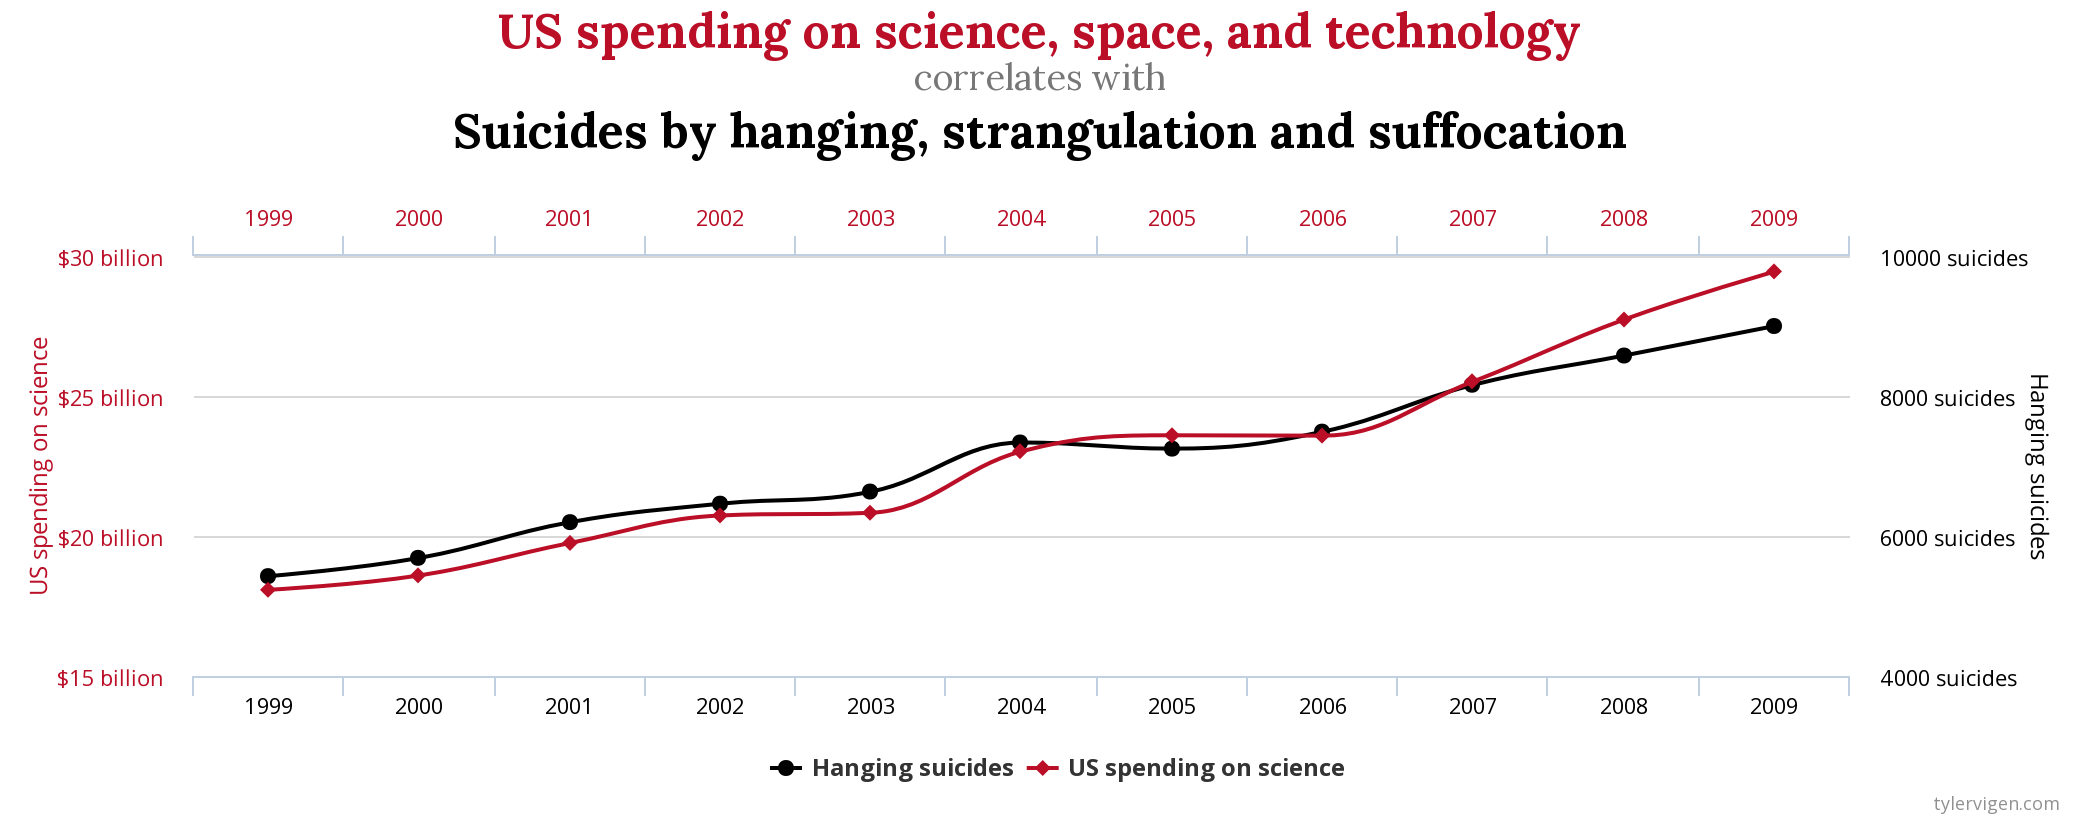
\includegraphics[width=\linewidth]{img/chart.png}
        \caption{Esempio di correlazione spuria da 
        \url{https://www.tylervigen.com/spurious-correlations}}
        \label{fig:spurious_relations}
    \end{center}
\end{figure}

Affidandoci solamente al grafico e ai dati riportati in 
figura, ci verrebbbe da pensare che le due categorie 
siano in qualche modo correlate, e che il governo 
americano debba essere fermato, in quanto respondabile di 
incitamento al suicidio.
Ebbene non è così, questo è un caso di relazione 
spuria \cite{wiki:Spurious_relationship}, ovvero che due o 
più variabili sono associate ma non causalmente correlate.

Associatività e causalità infatti non sono la stessa cosa,
ed è bene quando si studia l'una, non confondersi con l'altra
altrimenti tutto lo studio diverrebbe fallace e inutilizzabile.
In statistica, una correlazione tra dati è una qualsiasi 
relazione che vi è tra due o più variabili, sia essa di 
tipo causale oppure non \cite{wiki:Correlation}. 
Nell'esempio di prima la correlazione
tra le due variabili potrebbe essere banalmente il tempo, 
infatti con il passare del tempo la spesa media per la 
ricerca aerospaziale è continuata a salire per via 
del sempre più alto interesse e investimento nel settore
e sfortunatamente con il passare degli anni si è registrato
un aumento costante del numero di suicidi. 

Il bias che abbiamo verso la ricerca di un complicato intreccio
tra gli eventi, in maniera che questi siano sempre contigui
l'uno con l'altro, in maniera che si possa tracciare una 
chiara e distinta linea dal primo all'ultimo ci trae in 
inganno quando questi sembrano esserlo ma in realtà non lo sono.
Molto spesso la risposta più semplice è anche quella meno 
interessante, ma comunque corretta, ovvero che due eventi 
completamente slegati tra loro possono avere andamenti simili, 
così come differenti addendi possono portare lo stesso risultato; 
Solamente perchè cinque più cinque fa dieci non vuol dire che 
dieci sia il risultato solamente di cinque più cinque.

\begin{figure}[h]
    \begin{center}
        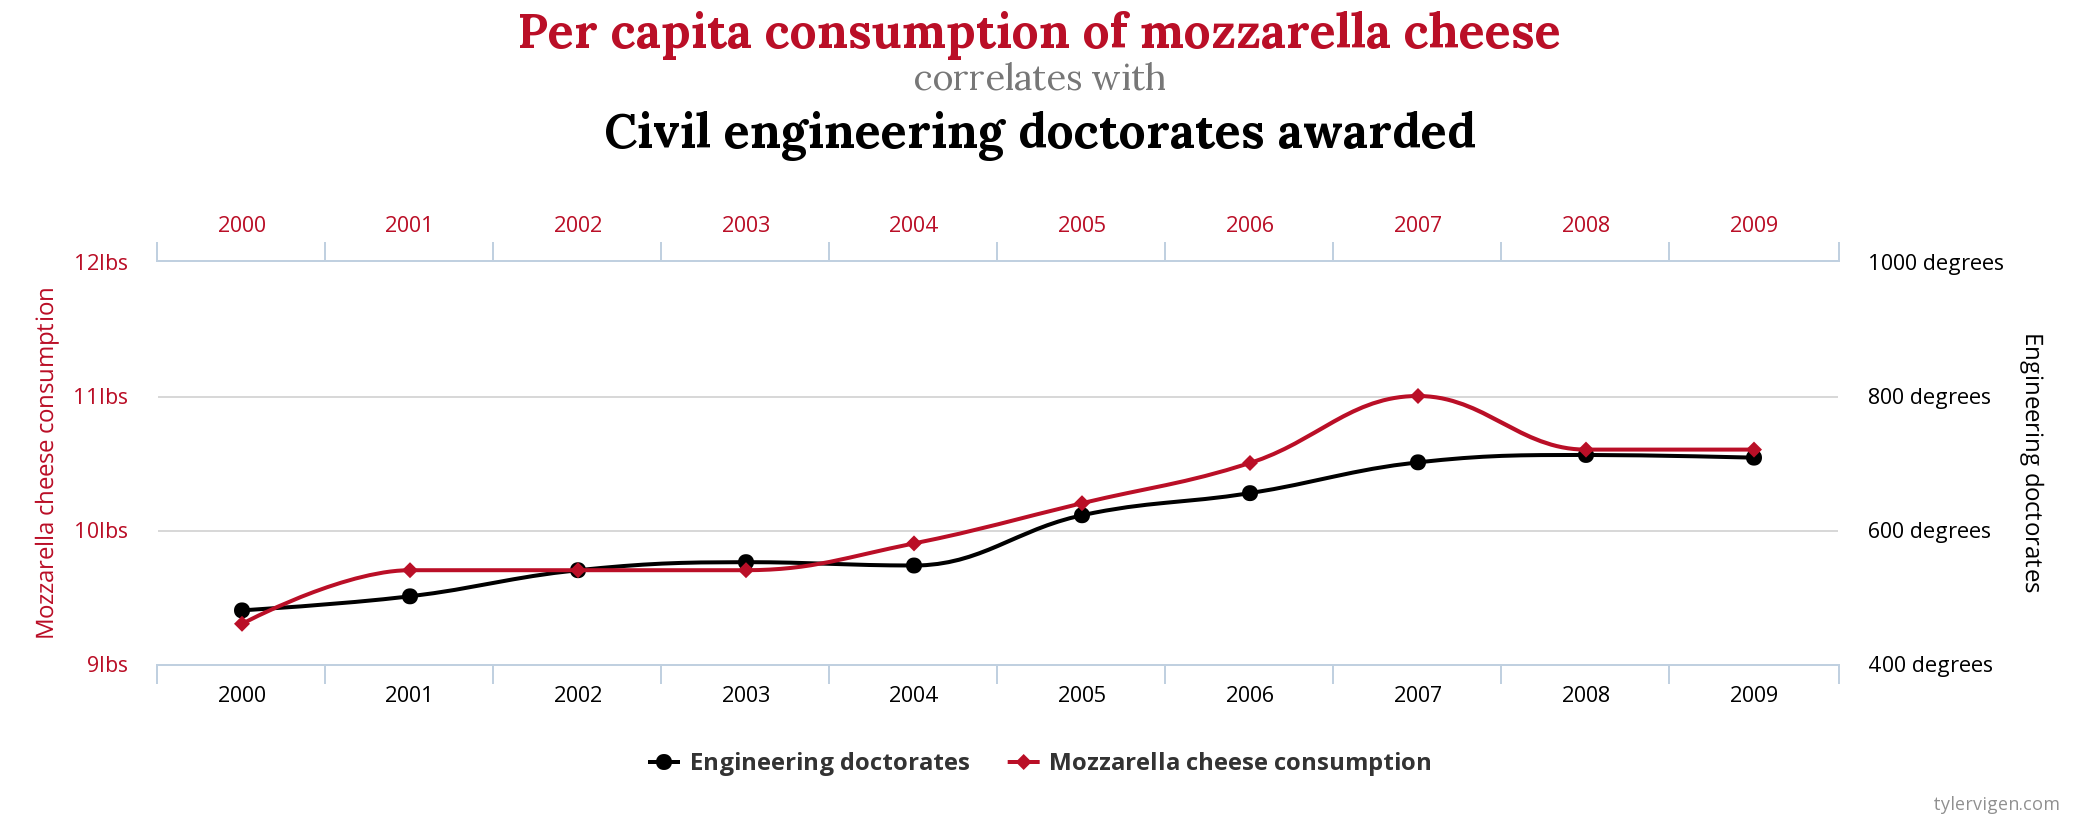
\includegraphics[width=\linewidth]{img/chart1.png}
        \caption{Un altro esempio di correlazione spuria da 
        \url{https://www.tylervigen.com/spurious-correlations}}
        \label{fig:another_spurious_relations}
    \end{center}
\end{figure}

\newpage

\subsection{Causalità}
Il problema della causalità non è da prendere sotto gamba
ed è uno dei problemi cardine quasi si vogliono determinare e 
applicare degli intervanti all'interno di una popolazione per
cercare di mitigare ad esempio la diffusione di un agente 
patogeno \cite{Parascandola2001-kw}. 

Come è stato già introdotto precedentemente, i dati sono
completamente muti ma siamo noi che dobbiamo imparare a 
capire il significato di ciò che esprimono. Un esempio 
estremamente calzante di come pur avendo bene in mente il
problema sopra citato delle correlazioni \emph{spurie}, si
possa comunque essere ingannati dai dati, è il seguente:

Poniamo di essere un medico e di dover decidere se 
prescrivere o meno ad un paziente un determinato medicinale.
Per aiutarci nella decisione abbiamo la storia clinica
del paziente e i risultati di uno studio su una nuova 
medicina che attesta di curare il malessere del paziente.
Questa nuova medicina è stata testata su un gruppo di 
settecento persone divise in due pari sottogruppi in cui 
350 pazienti decidevano autonomamente se prendere o meno 
la medicina e 350 decidevano autonomamente il contrario.
I risultati sono i seguenti:

\begin{figure}[h]
    \begin{center}
        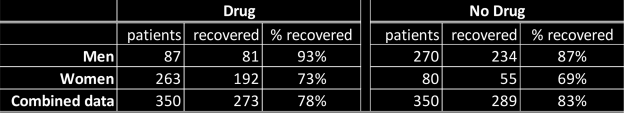
\includegraphics[width=\linewidth]{img/simpson.png}
        \caption{Risultati medicina}
        \label{fig:simpson_paradox}
    \end{center}
\end{figure}

Questi risultati sembrano suggerire come la prescrizione 
di questa nuova medicina non aiuti i pazienti a stare meglio.
Tuttavia questo risultato cade nel così detto \emph{paradosso di Simpson}
\cite{wiki:Simpson's_paradox} per cui i dati aggregati relativi 
ad uno specifico trattamento sembrano descrivere una sua 
perdita di efficacia relativamente ai singoli dati delle 
singole categorie in esame, portando un lettore non attento 
a cadere nell'inganno di pensare che ci sia una perdita di 
efficacia. Questo esempio pone l'accento sul fatto che non sempre
estrapolare informazioni da dei dati aggregati può risultare
efficace, e anzi, alle volte questi possono ingannare.
In questi casi bisogna estrapolare le informazioni di 
causalità dai dati singoli.

E' chiaro che non sia così semplice comprendere le cause 
di un determinato effetto, o insieme di effetti. Conoscere
l'agente patogeno, o quanto meno la sua natura può aiutare,
ma non sempre è sufficiente. L'utilizzo di modelli di 
Machine Learning per l'estrapolazione di dati, di correlazioni
e successivamente per la definizione di policy di intervento
può risultare in un rischio non indifferente ma al contempo 
descrive un potente alleato per la definizione di policy di 
intervento all'interno di settori estremamente delicati come 
quelli sanitari \cite{doi:10.1098/rsos.220638}.
% modelli compartimentali: deterministici e stocastici
\subsection{Modelli Compartimentali}
% scrivere stato dell'arte simile a chapter 2 pg.33 pdf book (download)
In epidemiologia i modelli compartimentali sono una tecnica di modellezione 
generica che si predispone molto bene allo studio complessivo del comportamento
di una malattia infettiva \cite{wiki:Compartmental_models_in_epidemiology}. 
Questa tecnica di modellazione si applica anche ad altre branche della 
scienza, una tra tutte la finanza.

Questa tecnica di modellazione matematica basa il proprio funzionamento 
sull'assunzione che, data una popolazione di individui, questi vengano 
etichettati in maniera differente, in base allo stato di progressione 
della malattia che hanno, o non hanno, contratto. Così facendo si vanno a 
definire dei compartimenti ben separati che possono interagire tra loro, ma 
che rimangono chiaramente distinti l'uni dagli altri.

\subsubsection*{Equazioni Ordinarie Differenziali}
Un equazione ordinaria differenziale (ODE) e' un equazione che coinvolge alcune derivate
ordinarie di una funzione. \cite{wiki:Equazione_differenziale_ordinaria} Generalmente data una 
derivata di una funzione si vuole studiare la funzione di partenza e per fare questo bisogna trovare 
l'antiderivata (o integrale) della funzione in esame. 

$$\frac{dx}{dt}(t) = cos(t) \rightarrow x(t) = sin(t) + C$$

Generalmente pero' risolvere una ODE e' piu' complicato di risolvere un semplice integrale, e pur sapendo 
che il principio alla base rimane la risoluzione di un integrale, la parte difficile e' quella di determinare
quale tipo di integrazione abbiamo bisogno per ricavare la nostra soluzione.

Fintanto che le equazioni associate a $\frac{dx}{dt}$ dipendono esclusivamente dalla variabile $t$ e non 
dalla funzione $x(t)$ allora la loro risoluzione risulta molto piu' facile di quanto non sembri. Tuttavia 
nel caso in cui si avesse una funzione che dipende da $x(t)$ questo ragionamento si fa piu' complicato.
Nel caso in cui $\frac{dx}{dt}$ dipende da $x(t)$ non e' possibile applicare una semplice integrazione e 
successivamente il teorema fondamenteale del calcolo \cite{wiki:Fundamental_theorem_of_calculus}, ma anzi 
necessitiamo di effettuare alcune manipolazioni, in particolare quelle che prendono il nome di \emph{chain rules}
o \emph{u-substitution}.

\subsubsection{Il modello Kermack-McKendrick}
Secondo la definizione precedente possiamo separare la popolazione soggetta di studio 
in categorie, o compartimenti, e assumere una relazione temporale che descriva il passaggio 
di individui da un compartimento all'altro. Malattie che garantiscono un immunita' avranno 
una struttura compartimentale differenti da malattie che non la garantiscono.

Il modello che tutt'ora viene usato come riferimento e come base per 
lo studio e modellazione è il così detto modello 
\textbf{Susceptible, Infectious, Recovered} (SIR)

\begin{figure}[h]
    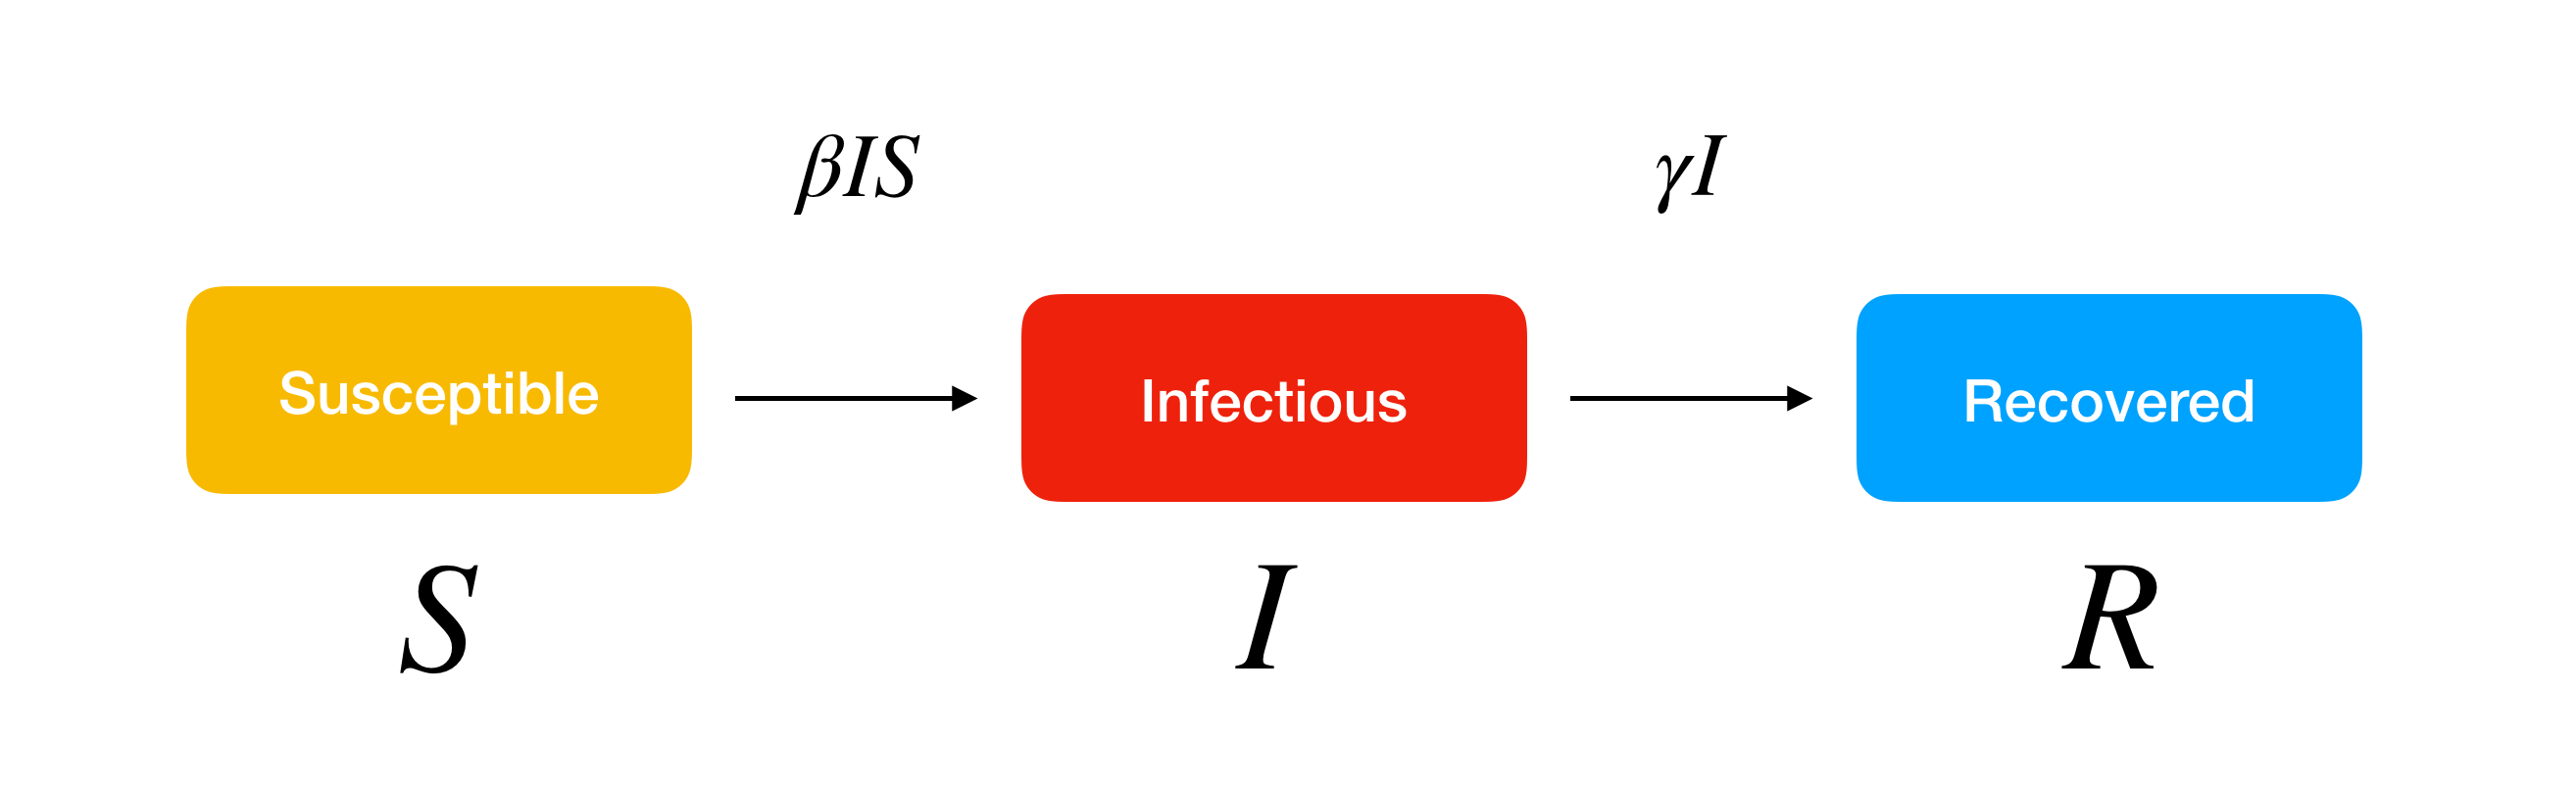
\includegraphics[width=\linewidth]{img/sir.png}
    \caption{Struttura modello SIR} 
    \label{fig:SIR_Structure}
\end{figure}

Questo modello è stato ideato all'inizio del 20esimo secolo, 
più precisamente nel 1927, da Kermack e McKendrick. Come introdotto questo modello
si basa sull'assunzione che all'interno di una popolazione durante 
il decorso di una malattia vi possano esistere solamente tre stadi in cui 
un individuo può essere inserito: 

\begin{itemize}
    \item Susceptible: Questo stadio rappresenta lo stato iniziale per la maggior parte
    degli individui all'interno di una popolazione. Rappresenta il numero di 
    persone che possono contrarre la malattia.
    \item Infectious: Questo stadio rappresenta tutti quegli individui che dallo 
    stato di Susceptible, dopo essere venuti in contatto con un individui infetto, 
    diventano a loro volta individui infetti.
    \item Recovered: Questo stadio rappresenta una duplice categoria, quella degli
    individui che alla fine del docorso della malattia sopravvivono ad essa, e 
    quelli che invece muoiono a causa di questa. Generalemente questo stato viene
    anche definito come Removed.
\end{itemize}

Da questa semplice idea poi si è andato a sviluppare un modello
matematico per descrivere come queste 3 categorie separate ma 
che si influenzano vicendevolmente, cambiano nel corso del tempo.
La variabile indipendente del modello e' il tempo, indicato come $t$ e il 
tasso di trasferimento tra compartimenti, il quale e' espresso matematicamente come 
derivate rispetto al tempo e alla dimensione del compartimento, e come risultato questo 
modello e' stato inizialmente formulato tramite l'utilizzo delle equazioni differenziali
\cite{Brauer2008}. 

Durante la formulazione del modello in termini di derivate della dimensione di ogni compartimento
si assume che il numero di individui di ogni compartimento sia rappresentabile come una funzione 
differenziabile nel tempo. Questa assunzione puo' essere una ragionevole approssimazione nel caso 
in cui vi siano molti individui per compartimento, altrimenti potrebbe risentire di essere sospetta
in caso contrario. Nel caso in cui si utilizzino le equazioni ordinarie differenziali come modello 
si assume che il comportamento della popolazione sia determinato completamente da una relazione deterministica. 
Questa assunzione puo' essere una ragionevole approssimazione, tuttavia esistono approcci di tipo 
\emph{stocastico} che aggirano questo tipo di assunzione introducendo concetti probabilistici per
la modellazione del modello.

Il modello in figura \ref{fig:SIR_Structure} e' un caso speciale del modello proposto da Kermack e McKendrick 
nel loro articolo del 1927, ma e' divenuto il modello base per la strutturazione di questo tipo di modelli.
Questa tipologia di modello descrive il seguente sistema di equazioni ordinarie differenziali:
$$\frac{dS}{dt} = -\beta \cdot S \cdot I$$
$$\frac{dI}{dt} = \beta \cdot S \cdot I - \gamma \cdot I$$
$$\frac{dR}{dt} = \gamma \cdot I$$

Questo sistema modella le seguenti assunzioni: 
\begin{itemize}
    \item In media un individuo della popolazione effettua sufficienti contatti con altri individui tale per cui 
    e' possibile far evolvere l'infezione con la seguente relazione $\beta \cdot N$ con $N$ numero di individui totali. 
    \item Gli infetti abbandonano il compartimento che determina gli infetti con un tasso pari a $\gamma \cdot I$.
    \item Non esistono entrate o uscite di individui dalla popolazione totale eccezione fatta per possibili uscite tramite morte
    data dalla malattia stessa.
\end{itemize}

Data la descrizione sopra fatta, in accordo con il primo punto, la probabilita' di un contatto casuale da un individuo 
infetto con un individuo suscettibile, a cui e' possibile trasmettere l'infezione, e' di $\frac{S}{N}$, sove il numero di nuovi 
infetti e' dato da $(\beta \cdot N) \cdot (\frac{S}{N}) \cdot I = \beta \cdot S \cdot I$. Questo approccio e' criticabile in quanto 
si puo' argomentare come il tasso di contatti dovrebbe essere governato dal numero di infetti e non dei suscettibili, andando 
cosi' a descrivere la seguente formula $(\beta \cdot N) \cdot (\frac{I}{N}) \cdot S = \beta \cdot S \cdot I$. In entrambi i casi 
si ottiene lo stesso tasso di infezione; tuttavia possono esistere approcci dove una scelta sia piu' adatta dell'altra.

La seconda assunzione non ha una chiara controparte con il mondo epidemiologico. Consideriamo l'insieme dei membri che sono stati infettati 
in un dato periodo di tempo e consideriamo $u(s)$ come il numero di questi che sono ancora infettivi dopo $s$ unita' di tempo. Se definiamo 
$\alpha$ come la frazione di infetti che abbandona la classe di appartenenza in un determinato periodo di tempo, otteniamo la seguente formula
$u' = - \alpha u$, la cui soluzione e' $u(s) = u(0) e^{-\alpha s}$. Con questo la frazione di infetti che rimangono infettivi dopo un periodo 
$s$ e' $e^{-\alpha s}$, per cui il periodo di infettivita' viene approssimato come una \emph{distribuzione esponenziale} con media 
$\int_{0}^{\infty} e^{-\alpha s} \,ds = \frac{1}{\alpha}$.

Questa assunzione, per cui il tasso di contatto e' proporzionale alla dimensione della popolazione $N$ con una costante di 
proporzionalita' $\beta$  e una distribuzione esponenziale del tasso di ripresa, e' generalmente troppo semplicistica. Tuttavia pur essendo 
un modello che descrive un andamento estremamente semplicistico e irrealistico, e' stato osservato come modelli molto piu' complessi e realistici 
hanno dimostrato comportamenti estremamente simili a questo, facendo si che questo modello, seppur semplice, sia un buon modello che approssima bene 
la realta'.

Il problema definito precedentemente non e' possibile da risolvere analiticamente, pero' da cio' e' possibile imparare il comportamento generale del sistema.
Questo approccio permette di inserire un numero variabile di infetti all'interno di una popolazione per studiare se e come 
un'epidemia si propaghi. La quantita' $\beta \cdot \frac{S(0)}{\alpha}$ e' indicata come una soglia generalmente conosciuta 
come \emph{basic reproduction number} e viene indicato come $R_0$, il quale determina se puo' o meno avvenire un'epidemia. 
Se $R_0 < 1$ allora l'infezione andra' a morire prima di diventare una epidemia, mentre se fosse $R_0 > 1$ vi sara' 
un outbreak epidemico.

L'indice $R_0$ definisce il numero di infezioni secondarie causate da un singolo individuo durante il proprio periodo infettivo 
all'interno di una popolazione pienamente suscettibile di dimensione $K \approx S(0)$ durante l'intero decorso dell'infezione. In 
questa situazioneun individuo infetto effettua $\beta \cdot K$ contatti per unita' di tempo, ognuno di essi con un individuo suscettibile 
che produce nuove infezioni durante un periodo medio infettivo di $\frac{1}{\alpha}$; con questo si puo' ottenere che il valore di $R_0$ e' 
$\beta \cdot \frac{K}{\alpha}$. Generalmente e' difficile stimare il rateo di contatto $\beta$ in una popolazione in quanto questo dipende fortemente 
dalla tipologia di malattia studiata ma anche dal comportamento sociale degli individui. Tuttavia esistono molteplici approssimazioni 
che permettono di modellare l'andamento di una malattia infettiva in presenza di pochi dati. 

Il numero di infetti e' stato osservato crescere esponenzialmente e questo puo' essere approssimato dalla seguente formula $I' = (\beta \cdot K - \alpha) \cdot I$
e l'iniziale crescita e' definibile come $r = \beta \cdot K - \alpha = \alpha \cdot (R_0 - 1)$. Il valore di $r$ puo' essere stimato sperimentalmente 
all'inizio di una pandemia. Successivamente, data la possibilita' di misurare sia $K$ che $\alpha$, $\beta$ puo' essere calcolato come 
$\beta = \frac{r + \alpha}{K}$, tuttavia questo approccio e' sensibile alla presenza di incompletezza dei dati e alla segnalazione parziale dei casi effettivi, andando 
ad avere una rappresentazione non accurata. Questa sensibilita' nell'accuratezza e' ulteriormente accentuata quando si studia l'outbreak di una malattia 
precedentemente sconosciuta o in cui i primi casi sono facilmente proni a diagnosi errate.   

\subsubsection{Derivazione modello SIR: modello SEIR}
In molteplici malattie infettive esiste un periodo definito di \emph{esposizione} \cite{wiki:Incubation_period} in cui un individuo una volta infetto non 
e' immediatamente infettivo per cui vi e' un ritardo nella trasmissione effettiva della malattia. Questo periodo e' irrilevante quando e' estremamente breve. 
Tuttavia un periodo di esposizione lungo puo' portare a differenze significative nel modello. Generalmenmte per modellare questa variante e' sufficiente 
inserire un nuovo compartimento \textbf{E} il quale va a modificare il sistema di equazioni differenziali nel seguente modo
$$\frac{dS}{dt} = - \beta \cdot (N) \cdot S \cdot I$$
$$\frac{dE}{dt} = \beta \cdot (N) \cdot S \cdot I - \kappa \cdot E$$
$$\frac{dI}{dt} = \kappa \cdot E - \gamma \cdot I$$
$$\frac{dR}{dt} = \gamma \cdot I$$

\begin{minipage}{\linewidth}
    \centering
    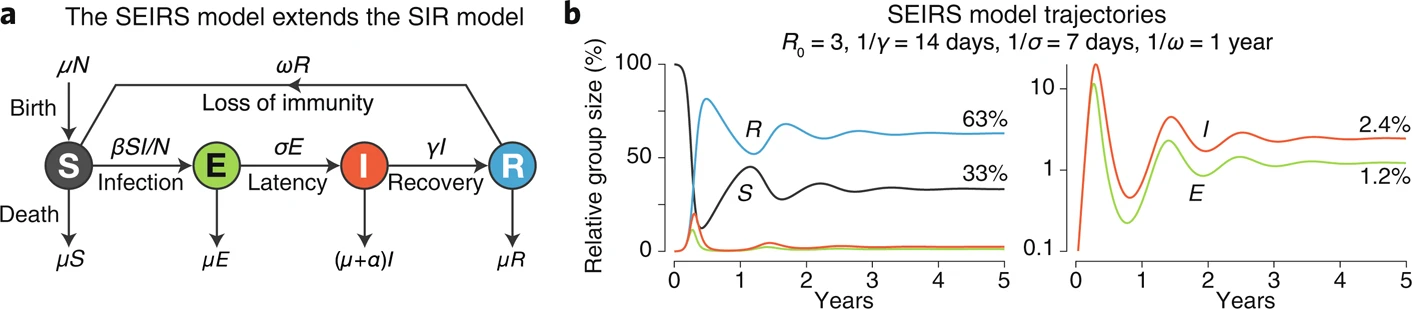
\includegraphics[width=\textwidth]{img/41592_2020_856_Fig1_HTML.png}
    \captionof{figure}{Modello SEIRS preso dall'articolo \cite{Bjornstad2020}}
    \label{fig:SEIRS_model}
\end{minipage}

Questo modello permette di integrare l'evenienza di casi \emph{asintomatici} i quali sono infettivi e non totalmente 
associabili al compartimento \textbf{E}.

\subsubsection{Modello SIR stocastico}
Una delle assunzioni del modello presentato precedentemente, ovvero della tipologia \textbf{deterministica} e' quella per cui la dimensione 
dei compartimenti e' abbastanza grande da permettere di avere un mix omogeneo di membri al suo interno. Fintanto che questa assunzione e' sufficientemente
ragionevole quando un'epidemia e' gia' avviata, all'inizio la situazione puo' riszultare estremamente differente. Fintanto che all'inizio di una 
epidemia la maggior parte della popolazione ricade all'interno della categoria suscettibile, ovvero che non e' stata (ancora) infettata, e il numero associato 
agli individui infetti e' relativamente piccolo. Il rateo di trasmissione della malattia dipende fortemente dal pattern dei contatti tra individui e servirebbe utilizzare 
una descrizione di questo pattern. Poiche' il numero di infetti e' piccolo una descrizione del modello che utilizza una assunzione di \emph{mass action} dovrebbe essere 
sostituito da un modello che incorpora degli effetti stocastici.

\begin{minipage}{\linewidth}
    \centering
    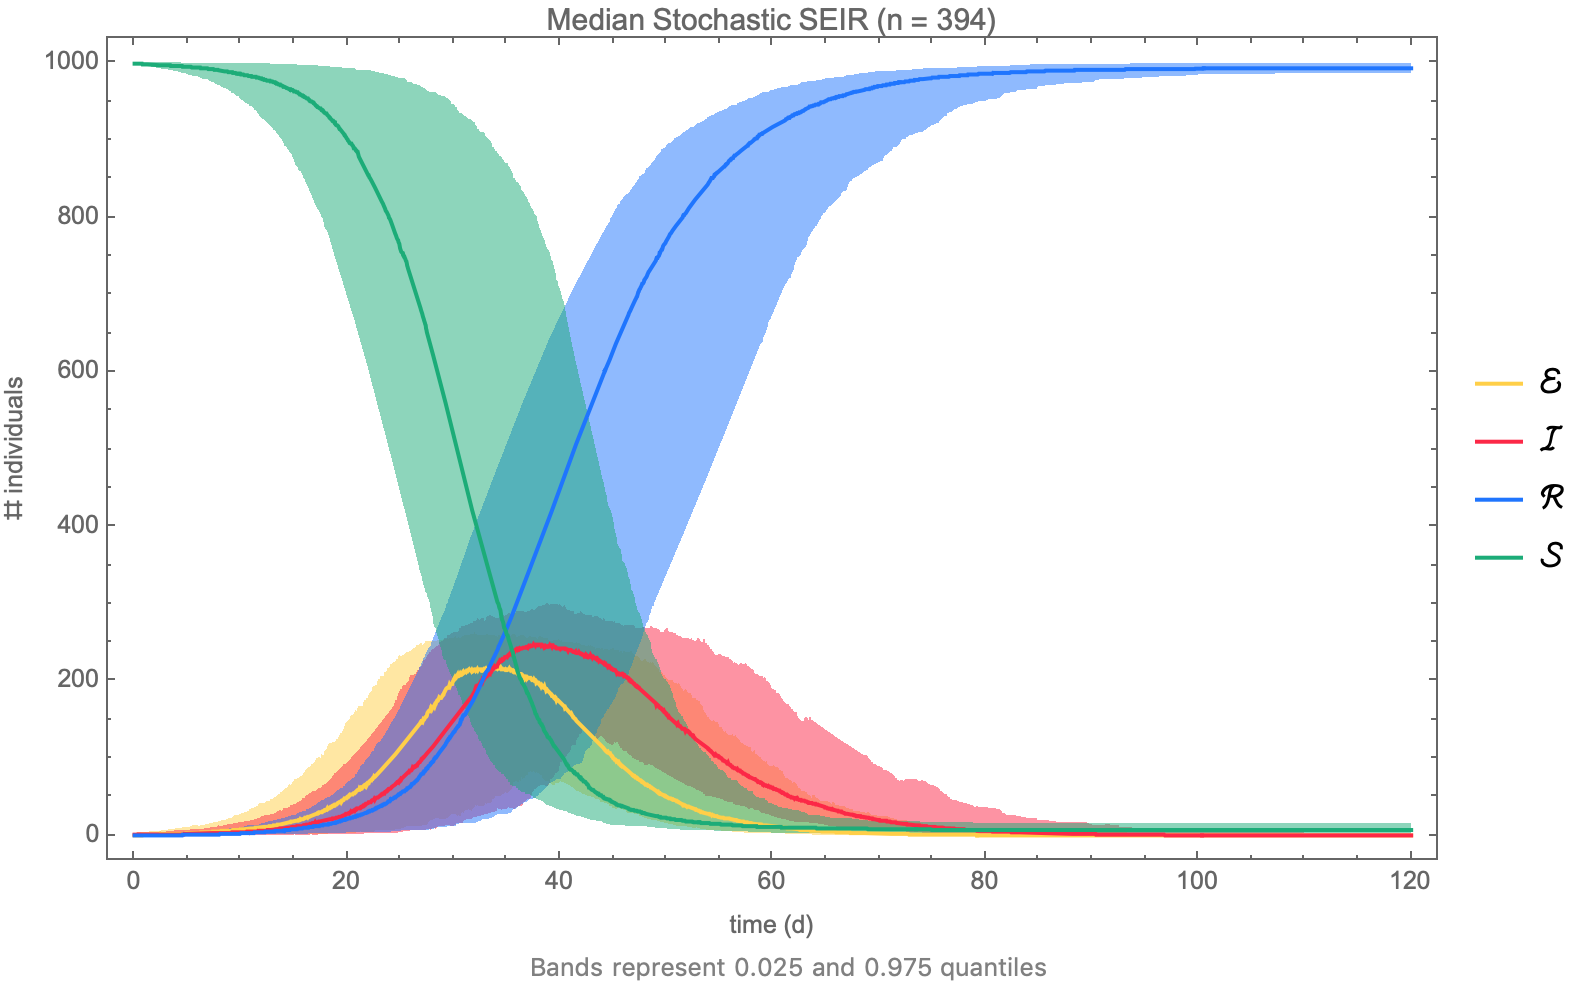
\includegraphics[width=\textwidth]{img/stochastic_SEIR.png}
    \captionof{figure}{Modello SEIRS stocastico}
    \label{fig:stochastic_SEIR_model}
\end{minipage}

% modelli ad agente: discreti e continui in spazio e tempo
\subsection{Modelli ad Agente}
% scrivere sezione simile ad articolo (download)
Un modello ad agente e' un modello computazionale per la simulazione delle 
azioni e interazioni di un insieme di agenti autonomi, siano essi individui
o gruppi di individui, con l'obiettivo di comprendere il comportamento 
del sistema e la relazione che vige con i suoi risultati \cite{wiki:Agent-based_model}
\cite{7822080}.

\begin{minipage}{\linewidth}
    \centering
    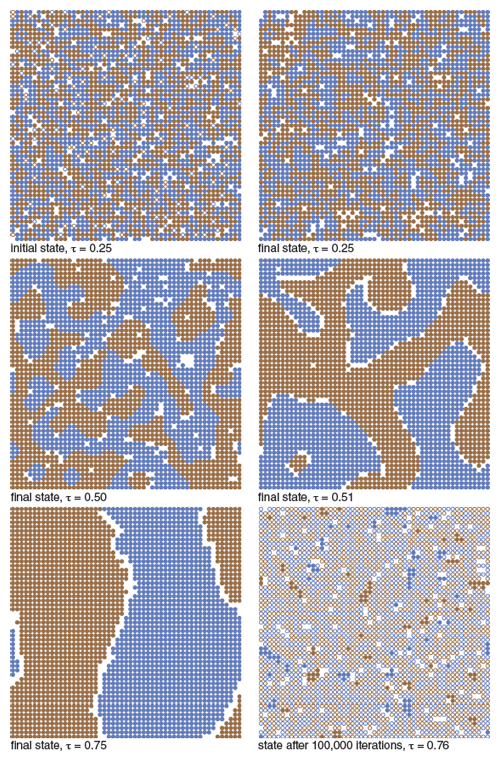
\includegraphics[scale=0.5]{img/201381146479794-2013-09HayesF1png.png}
    \captionof{figure}{Schelling's model of segregation simulato tramite ABM}
    \label{fig:schelling_segregation_abm}
\end{minipage}

L'utilizzo di modelli ad agente in epidemiologi e' una tecnica nota che 
da piu' di un decennio viene impiegata per simulare e comprendere le 
situazioni e i problemi piu' disparati, tutti pero' generalmente accomunati
dal fatto che come parametro portante vi sia il comportamento umano \cite{Groff2019}
\cite{El-Sayed2012-ac} \cite{Tracy2018-lc} \cite{Bissett2021}. 
Uno dei parametri piu' caratterizzanti che da sempre sono stati tenuti 
in considerazione e assunti come ristretti ad una piccola cerchia, sono 
le interazioni sociali tra individui. Questo sovrainsieme di parametri 
racchiude molteplici sottoinsiemi di parametri che descrivono delle 
interazioni piu' specifiche ma che possono essere raggruppate come macro 
categoria se si scende a compromessi. 

Questa specifica e' importante in quanto uno delle sfide piu' grandi che 
il mondo della simulazione, e quindi quello epidemiologico devono affrontare
e' proprio quello di trovare un modo efficiente e soprattutto realistico 
di simulare le interazioni sociali tra individui, in quanto queste possono
influenzare notevolmente i risultati di una simulazione definendola utile
oppure inutile \cite{Silverman2021}. Non soltanto, un'altra sfida e' il modo 
con cui si decide di rappresentare lo spazio (e il tempo) all'interno della
simulazione. In base al tipo di discretizzazione effettuata una simulazione
potrebbe essere utile in un campo ma totalmente inutile in un altro 
\cite{KONSTANTINOUDIS2020100319}.

\begin{minipage}{\linewidth}
    \centering
    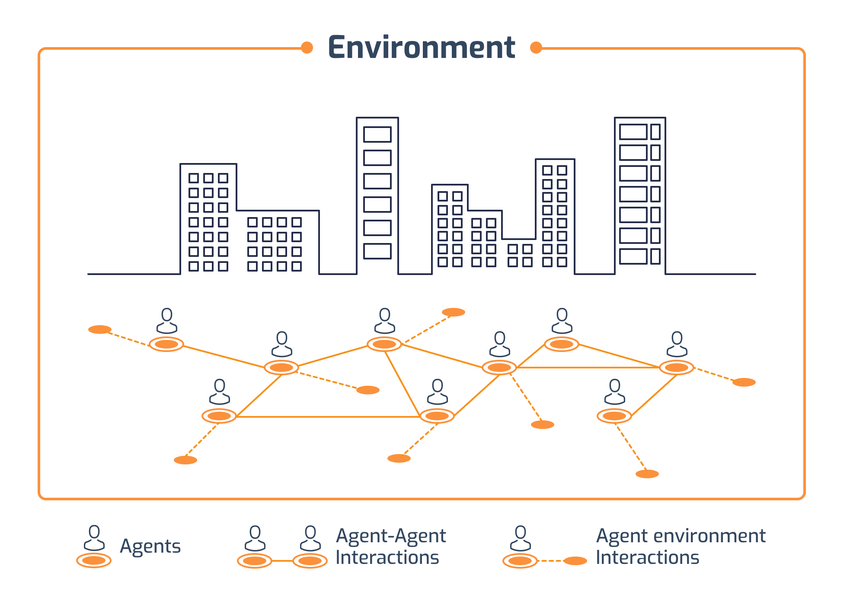
\includegraphics[scale=0.5]{img/Schematic-representation-of-an-agent-based-model-ABM.png}
    \captionof{figure}{Rappresentazione schematica di un modello ad agente}
    \label{fig:schematic_representation_abm}
\end{minipage}

Con l'arrivo della pandemia da COVID-19 molti ricercatori hanno 
focalizzato la propria attenzione sull'idea di sviluppare un modello 
ad agente puro oppure ibrido \cite{Marzban2021-pd}
(ibridato con delle ODE oppure delle Partial DE), con l'obiettivo di 
trovare un modello di simulazione in grado di simulare in maniera 
affidabile il decorso di una pandemia tenendo in considerazione le 
variabili piu' stocastiche e imprevedibili come il comportamento umano.
L'ambiente di lavoro simulato era generalmente un ambiente controllato
che poteva essere una citta' come in \cite{PRAJAPATI20232299}, 

Un'altro obiettivo e' quello di osservare l'impatto degli interventi non 
farmaceutici sulla popolazione come riporta \cite{NOVAKOVIC2022108790}
\cite{10.1371/journal.pcbi.1009149}.
Altri ancora invece utilizzano l'approccio simulativo tramite modelli ad 
agente per estrapolare delle ODE tramite l'analisi del modello, come
riportato da \cite{Nardini2021-pu}. 

\subsubsection{Discretizzazione}
La tematica della discretizzazione e' una delle proprieta' fondamentali
e al contempo uno dei problemi atavici della simulazione.
Il mondo in cui viviamo e' un mondo continuo, ma gli strumenti
che attualmente abbiamo per simularlo sono discreti, per cui 
ogni qualvolta che vogliamo simulare un evento dobbiamo decidere 
in che modo adattare la realta' alla simulazione, andando 
inequivocabilmente a perdere informazioni nel processo 
\cite{KONSTANTINOUDIS2020100319}. 

\begin{minipage}{\linewidth}
    \centering
    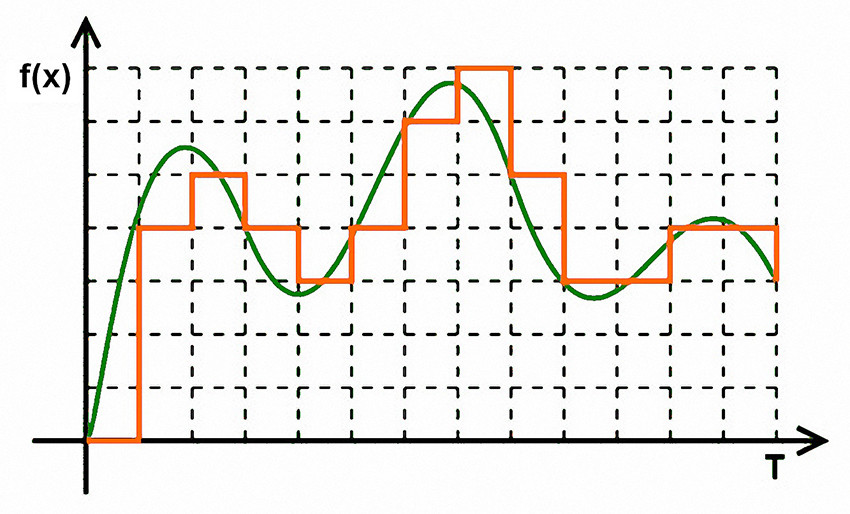
\includegraphics[scale=0.5]{img/figura-1-analogico-e-digitale-7ae2c4b25c8751e9a3771f91f1e65bb1f.jpg}
    \captionof{figure}{Esempio di discretizzazione dei dati}
    \label{fig:discretization}
\end{minipage}

Il processo di discretizzazione in una simulazione puo' prendere 
principalmente due macro aree che sono: lo spazio e il tempo. 
Molti framework di simulazione implementano al loro interno 
diversi trucchetti per simulare in maniera quanto piu' accurata
un insieme di dati continuo, permettendo all'utente di utilizzare
parole chiave come ad esempio ContinuousSpace. Quello che praticamente
viene fatto e' creare un ambiente per il modello che e' il piu'
preciso e granulare possibile, per cui servono allo scopo fintanto
che quest'ultimo non richiede una maggiore precisione. 

Il processo di discretizzazione comunque non e' sempre negativo, 
in quanto alcuni problemi possono essere simulati in maniera 
estremamente fedele anche effettuando questi accorgimenti, e anzi
alle volte non e' perfino necessario avere una precisione troppo 
alta per la simulazione di determinati eventi.

Se ad esempio si volesse simulare tramite un agente una partita 
a Risiko, non e' necessario richiedere uno spazio e un tempo continuo
della simulazione, in quanto questi possono essere rimpiazzati 
dalla loro controparte discreta che sono caselle e turni. 

\begin{minipage}{\linewidth}
    \centering
    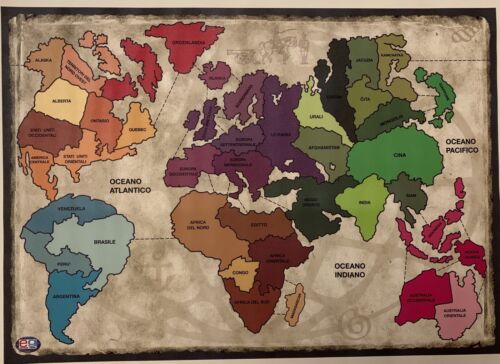
\includegraphics[scale=0.5]{img/s-l500.jpg}
    \captionof{figure}{Plancia di gioco di Risiko}
    \label{fig:risiko}
\end{minipage}

Se si volesse simulare il traffico aereo si potrebbe utilizzare
uno spazio a grafo dove ogni nodo rappresenta un aeroporto e 
gli archi rappresentano la tratta in partenza o in arrivo. Anche in 
questo caso l'applicazione della discretizzazione non sarebbe 
qualcosa di problematico.
% julia
\subsection{Julia}

Julia è un linguaggio di programmazione ad alto livello, 
multi-paradigma e open-source ideato per compiere analisi 
numerica ed effettuare operazioni di computer science in 
maniera rapida e stabile. Julia è nato ufficialmente come 
linguaggio di programmazione nell’anno 2012 con lo scopo di 
fornire uno strumento potente, robusto e veloce tanto se non 
più dei linguaggi considerati in questo ambito lo stato 
dell’arte, ovvero C e Fortran;  ma anche facile da approcciare, 
al contrario dei linguaggi sopra citati. Julia è un linguaggio 
di programmazione scritto in C++ e Scheme, ma gran parte della 
sua composizione è scritta in Julia stesso 
\cite{wiki:Julia_(programming_language)}.

le caratteristiche principali di questo linguaggio sono 
principalmente:
\begin{itemize}
    \item Alte performance: lo scopo per cui Julia è nato è 
    stato quello di offrire un linguaggio estremamente 
    performante con la capacità di poter compilare programmi 
    in codice nativo per molteplici piattaforme grazie 
    all’utilizzo di LLVM
    \item Dinamico: la scelta di rendere Julia un linguaggio 
    dinamicamente tipizzato lo rende di facile utilizzo in 
    quanto rende molto più semplice il suo approccio anche a 
    chi non ha una base solida di programmazione, in quanto 
    ritorna la stessa sensazione di immediatezza di un 
    linguaggio di scripting. Inoltre questo permette un alto 
    supporto per l’uso interattivo
    \item Ambiente riproducibile: lo scopo del linguaggio è 
    quello di poter permettere all’utente di ricreare le 
    stesse condizioni ogni volta su ogni macchina su cui un 
    programma viene eseguito. Questo può essere ottenuto 
    tramite l’utilizzo di file binari pre compilati
    \item Componibile: Julia utilizza l’approccio multiple 
    dispatch come paradigma, permettendo una grande 
    flessibilità nell’esprimere una elevata quantità di 
    pattern di programmazione, dall’object-oriented al 
    funzionale
    \item General Purpouse: lo scopo del linguaggio è quello 
    di creare un ecosistema in grado di poter soddisfare 
    qualsiasi esigenza di un utente, permettendo la creazione 
    di applicativi e microservizi senza dover ricorrere ad 
    integrazioni con codice non nativo Julia
    \item Open source: Julia abbraccia la filosofia open source, 
    e il codice sorgente dell’intero linguaggio, così come di 
    tutte le librerie è disponibile sulla piattaforma GitHub 
    sotto la licenza MIT. Questo permette una crescita 
    eterogenea grazie al contributo di più di 1000 utenti 
    che si impegnano a migliorare il linguaggio
\end{itemize}

\subsubsection{Agents.jl}
Seguendo la filosofia propria del linguaggio di programmazione 
in cui è sviluppata, la libreria Agents.jl \cite{Agents.jl} 
è stata sviluppata con l’idea di essere facile da imparare e 
usare ed estendibile, con forte attenzione sulla creazione ed 
evoluzione di modelli veloci e soprattutto scalabili. 
Molteplici esempi comparativi sono stati effettuati mostrando 
come il framework sviluppato permetta di avere un notevole 
guadagno prestazionale rispetto ai maggiori competitor 
attualmente presenti sul mercato (Mesa, Netlogo, MASON) 
\cite{ABAR201713}.

La facilità di interazione con questa libreria non è da 
confondersi con una mancanza di opzioni durante lo sviluppo, 
in quanto nativamente Agents.jl permette l’integrazione con 
altre librerie che in maniera altrettanto semplice e veloce 
offrono all’utente la possibilità 
di addentrarsi nel mondo del machine learning, in particolar 
modo il mondo del Scientific Machine Learning 
\cite{rackauckas2017differentialequations}, 
branca che soprattutto grazie alla pandemia da Covid-19 ha 
visto un enorme interesse per l’analisi di dati per lo 
sviluppo di policy di prevenzione e contenimento della 
pandemia. 

\subsubsection{SciML.ai}
SciML è una collezione di librerie dedite al calcolo scientifico 
e non solo al machine learning. Questo framework permette di 
avere tutti gli strumenti per poter utilizzare facilmente, 
velocemente e in maniera robusta tecniche di analisi numerica 
molto avanzata, così da poter sviluppare applicazioni 
semplicemente senza essere banali 
\cite{rackauckas2017differentialequations} 
\cite{rackauckas2019diffeqflux} 
\cite{rackauckas2020universal}. 

Durante la pandemia da Covid-19 questo framework è stato 
utilizzato per sviluppare applicazioni le quali grazie 
all’utilizzo di tecniche di scientific machine learning 
riuscivano sia a prevedere in maniera molto accurata 
l’andamento dell’epidemia seppur in presenza di una scarsa 
quantità di dati (uno dei grandi problemi dei modelli di 
machine learning e di artificial intelligence sono gli enormi 
dataset necessari per addestrare le reti in maniera robusta) 
e le stesse presentavano misure di contenimento e prevenzione 
che si sono dimostrate essere efficaci 
\cite{10.1371/journal.pdig.0000142} \cite{DANDEKAR2021100220}. 

\subsubsection*{SafeBlues}
Un esempio di un modello di scientific machine learning può 
essere il modello denominato SafeBlues 
\cite{10.1371/journal.pdig.0000142} il quale simulando una 
rete bluetooth in cui gli individui potevano venire infettati 
da un virus e poi infettare a loro volta tutti gli individui 
nella rete con una certa probabilità, aveva riprodotto 
fedelmente l’andamento della pandemia da Covid-19. 
In aggiunta questa soluzione, aveva mostrato come 
l’applicazione di policy per il contenimento del virus 
bluetooth erano perfettamente applicabili anche al caso 
reale della pandemia. 

% neuralode
\subsection{Equazioni Neurali Differenziali}

La tecnica delle Equazioni Neurali Differenziali 
(END) ha attirato notevole attenzione, portando all'ibridazione di due 
paradigmi di modellazione distinti: le Equazioni Differenziali Ordinarie 
(ODE) e le reti neurali (NN). Questo sforzo mira a sfruttare al meglio 
entrambi i paradigmi, minimizzando gli effetti indesiderati \cite{chen2019neural} \cite{Kim_2021}.

Un'Equazione Differenziale è un metodo per specificare una trasformazione 
non lineare arbitraria, codificando matematicamente le ipotesi strutturali 
a priori del sistema. Esistono tre approcci comuni per definire tale 
trasformazione non lineare:

\begin{itemize}
    \item \textbf{Modellazione diretta}
    \item \textbf{Machine learning}
    \item \textbf{Equazioni differenziali}
\end{itemize}

L'approccio di modellazione diretta funziona solo quando si conosce 
la funzione esatta che collega l'input con l'output. Tuttavia, nella 
maggior parte dei casi, questa relazione è sconosciuta a priori, 
rendendo impossibile applicare questo metodo. In questi casi, l'approccio 
di machine learning diventa una soluzione valida.

\begin{figure}[H]
    \begin{center}
        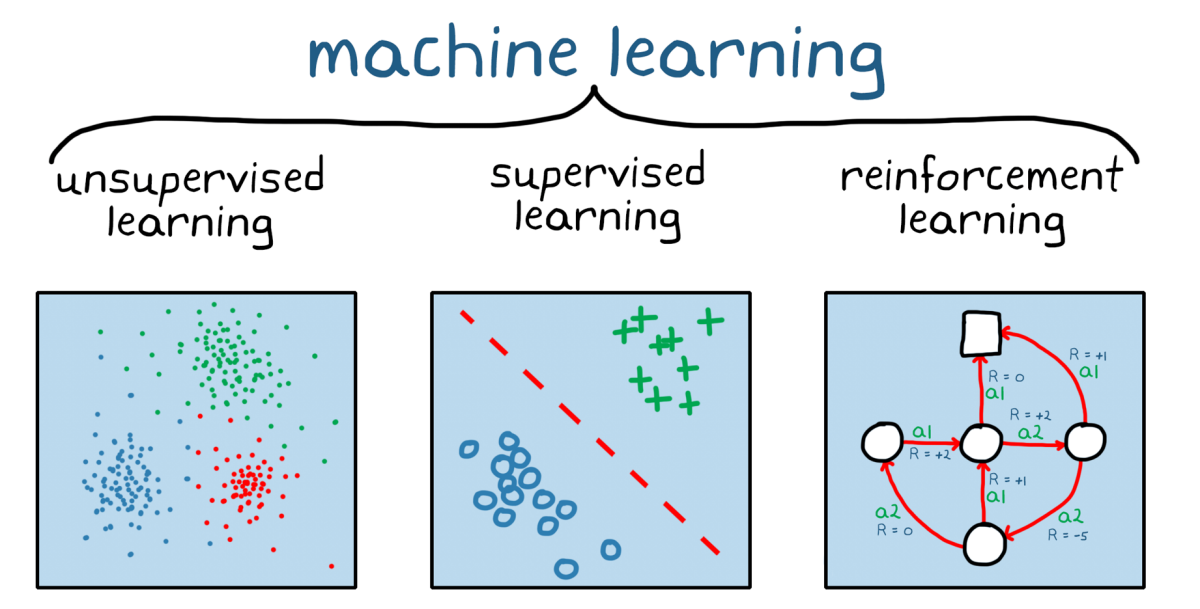
\includegraphics[width=\textwidth]{img/1689243301131.png}
        \caption{Differenti approcci di apprendimento di machine learning}
        \url{https://it.mathworks.com/discovery/reinforcement-learning/_jcr_content/mainParsys3/discoverysubsection/mainParsys/image.adapt.full.medium.png/1689243301131.png}
        \label{fig:ML_example}
    \end{center}
\end{figure}

Nel contesto generale del machine learning, dato un insieme di dati $x$, 
l'obiettivo è predire un insieme $y$ di dati correlati utilizzando una 
funzione sottostante. Questa funzione viene comunemente chiamata modello. 
Si inizia con una fase di addestramento in cui si cercano di regolare i 
parametri (iperparametri) del modello per ottenere un modello in grado di 
generare previsioni accurate. Successivamente, il modello viene utilizzato 
per inferire dati $x$ mai visti in precedenza. In sostanza, questo 
approccio consiste in una serie di trasformazioni non lineari.

L'uso del machine learning è affascinante perché si basa su un concetto 
estremamente semplice ma potente: adattare il modello ai dati forniti in 
modo efficace. Questa idea si estende ulteriormente alle reti neurali (NN), 
che sono essenzialmente insiemi di moltiplicazioni tra matrici seguite 
dall'applicazione di una funzione di attivazione. Ad esempio, una 
semplice rete neurale a tre strati è definita come:

$$ML(x) = \sigma(W_3 \cdot \sigma(W_2 \cdot \sigma(W_1 \cdot x)))$$

Dove $W_1$, $W_2$, e $W_3$ sono parametri apprendibili. L'obiettivo è 
selezionare questi parametri in modo che $ML(x) = y$ si comporti in modo 
simile alla funzione incognita che si desidera adattare. Grazie 
all'applicazione del teorema di approssimazione universale, si afferma 
che con un numero sufficientemente grande di parametri o strati, è 
possibile approssimare qualsiasi funzione non lineare in modo 
sufficientemente preciso.

\begin{figure}[H]
    \begin{center}
        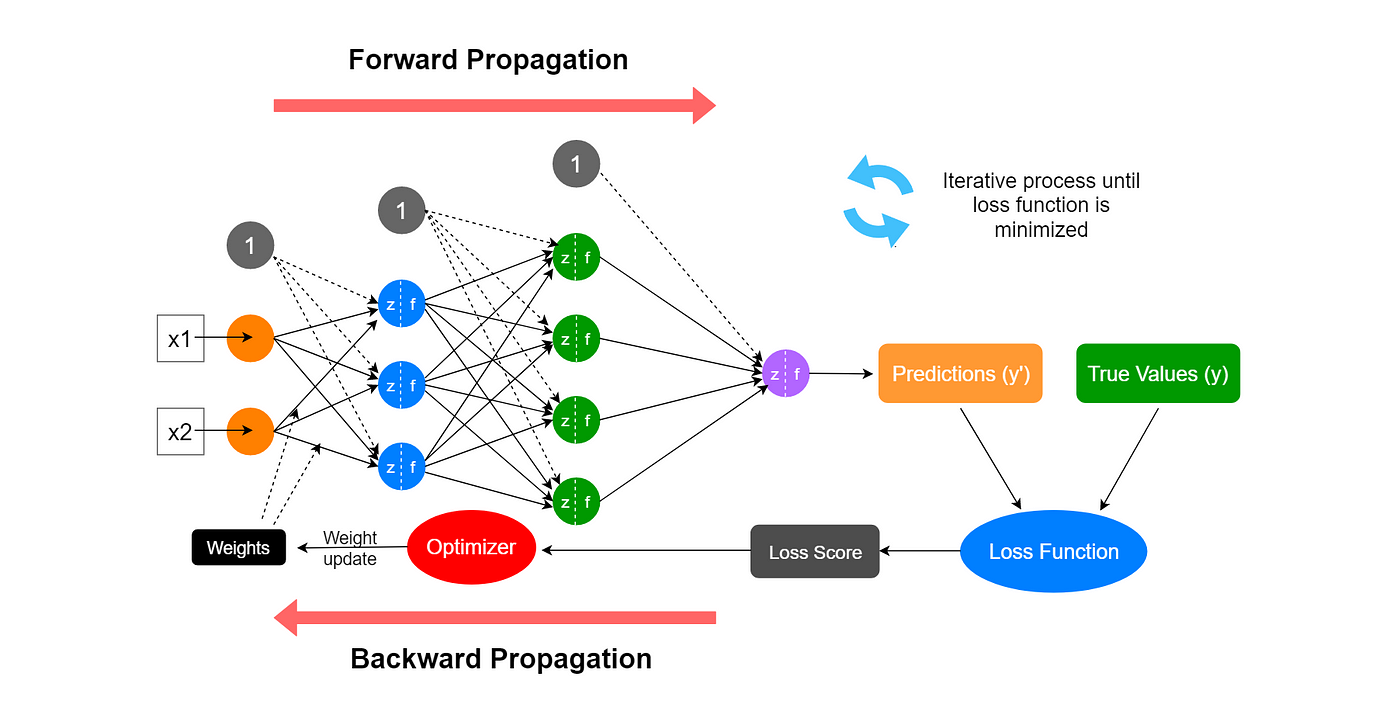
\includegraphics[width=\textwidth]{img/1_ZXAOUqmlyECgfVa81Sr6Ew.png}
        \caption{Esempio di funzionamento di una rete neurale}
        \url{https://miro.medium.com/v2/resize:fit:4800/format:webp/1*ZXAOUqmlyECgfVa81Sr6Ew.png}
        \label{fig:NN_example}
    \end{center}
\end{figure}

Questo approccio richiede l'apprendimento di ogni aspetto della 
trasformazione non lineare direttamente dai dati disponibili. 
In molti casi, però, non è possibile conoscere l'intera equazione non 
lineare, ma forse se ne conosce la struttura generale. Un modo per 
definire matematicamente questo tipo di approccio è attraverso le 
equazioni differenziali. Un metodo immediato è quello di definire un 
modello matematico in cui si cerca di apprendere una costante associata al 
comportamento di un insieme di dati:

$$y'(t) = \alpha \cdot y(t)$$

Questo approccio non richiede la conoscenza della soluzione dell'equazione 
differenziale per convalidare la correttezza del modello. La struttura del 
modello e la matematica stessa sono incorporate nel modello stesso, il 
quale successivamente produce una soluzione. Questo tipo di modelli è 
essenzialmente un insieme di equazioni che descrivono il cambiamento 
delle variabili nel tempo, con la soluzione dell'equazione differenziale 
come risultato finale.

\begin{figure}[H]
    \begin{center}
        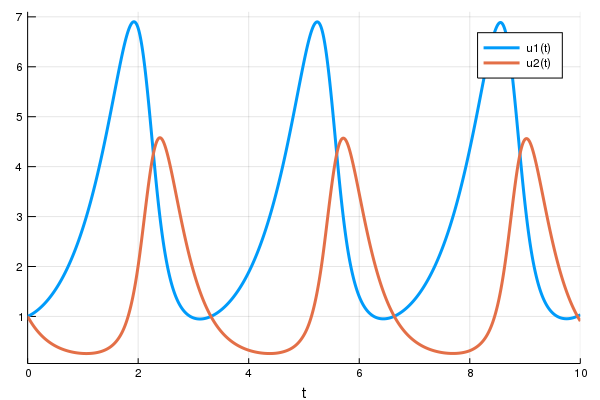
\includegraphics[width=\textwidth]{img/lotkavolterra.png}
        \caption{Esempio grafico ODE rappresentante la famosa equazione di Lotka-Volterra}
        \label{fig:lotkavolterra_example}
    \end{center}
\end{figure}

Questo metodo è stato ampiamente utilizzato in campi scientifici, e 
recentemente ha visto ulteriori sviluppi tramite l'integrazione di 
strutture matematiche aggiuntive che permettono di modellare sistemi 
complessi come quelli in ambito farmacologico o biologico.

Ciò che rende i modelli di machine learning interessanti è la loro fame 
di dati e la necessità di un grande insieme di dati di allenamento. 
In questo contesto, l'uso delle equazioni differenziali è diventato 
una scelta interessante per specificare la non linearità in modo 
apprendibile (tramite parametri) in modo più efficiente. Questo permette 
di incorporare la conoscenza specifica di un dominio nelle relazioni 
strutturali tra input e output del modello.

Un'Equazione Differenziale Neurale (Neural ODE) rappresenta un modo per 
collegare i mondi del machine learning e delle equazioni differenziali. 
L'approccio generale è quello di non apprendere solo la trasformazione 
non lineare tra i dati, ma anche la struttura stessa della 
trasformazione non lineare. Invece di avere il modello $y = ML(x)$, 
si ha il modello $y' = ML(x)$, e successivamente si tenta di risolvere 
l'equazione differenziale associata.

L'approccio fondamentale qui è che definendo il modello in questo modo e 
utilizzando un risolutore semplice e propenso agli errori come il metodo 
di Eulero, è possibile ottenere risultati equivalenti a quelli ottenuti 
con una ResNet \cite{he2015deep}. L'idea di base è che invece di 
modellare una rete neurale con sempre più strati, diventando sempre 
più profonda, è sufficiente modellare direttamente il sistema di 
equazioni differenziali e risolverlo con un risolutore specifico.

Questo approccio è efficiente dal punto di vista della memoria, è in 
grado di gestire dati irregolari, ha una forte conoscenza a priori 
dello spazio del modello, è in grado di approssimare sia funzioni 
lineari che non lineari e si basa su solide basi teoriche derivanti da 
entrambi i lati.

\subsubsection{Equazioni Differenziali Universali}

Recentemente, gli sviluppi nel campo del machine learning sono stati 
guidati dalle tecniche di deep learning, che richiedono grandi quantità 
di dati, noti come "big data", per risolvere problemi precedentemente 
considerati difficili e complessi, come il riconoscimento di immagini o 
il processing del linguaggio naturale.

Tuttavia, in molti settori, specialmente nella medicina e in altre 
discipline correlate, è difficile ottenere un insieme di dati 
sufficientemente ampio e diversificato per applicare queste tecniche. 
In questi contesti, i modelli meccanicistici rimangono la scelta 
principale. L'approccio data-driven dei modelli di machine learning, 
tuttavia, offre maggiore flessibilità e la possibilità di evitare 
ipotesi semplificative richieste dai modelli teorici.

\begin{figure}[H]
    \begin{center}
        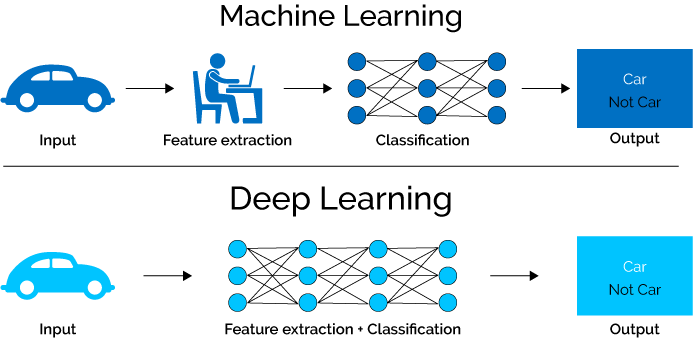
\includegraphics[scale=0.4]{img/Caratteristiche-e-funzionamento-del-Deep-Learning-in-informatica.png}
        \caption{Esempio comparativo tra funzionamento Machine Learning e Deep Learning}
        \url{https://goodboychan.github.io/images/copied_from_nb/image/fe.png}
        \label{fig:ml_dl_example}
    \end{center}
\end{figure}

Un'Equazione Differenziale Universale (UDE) è definita da un 
"approssimatore universale", un oggetto parametrico in grado di 
rappresentare qualsiasi funzione dati un certo numero di parametri. 
Gli approssimatori universali includono, ad esempio, le serie di Fourier 
o di Chebyshev per spazi a basse dimensioni e le reti neurali per spazi 
ad alta dimensione \cite{rackauckas2020universal}.

Un'UDE è un sistema di equazioni differenziali o algebriche non triviali 
che può approssimare qualsiasi funzione continua su un intervallo a 
qualsiasi livello di precisione desiderato. In altre parole, un'UDE è 
in grado di rappresentare qualsiasi sistema dinamico continuo con 
qualsiasi grado di dettaglio richiesto.

L'approccio delle UDE può essere accoppiato con tecniche data-driven, 
come l'algoritmo SINDy (Sparse Identification of Non-linear Dynamics), 
per l'identificazione sparsa di dinamiche non lineari in sistemi 
complessi come dinamiche dei fluidi o reti biologiche \cite{datadrivendiffeq}.

\begin{figure}[H]
    \begin{center}
        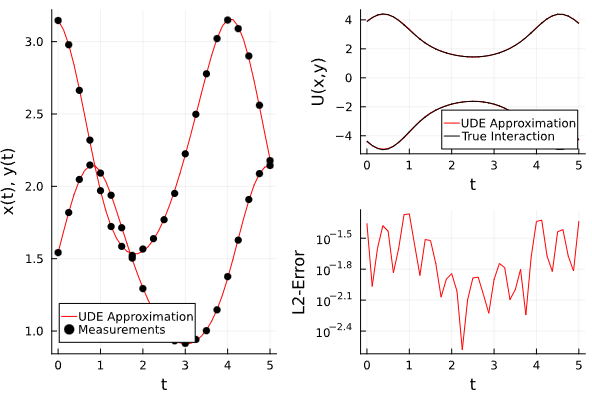
\includegraphics[scale=0.35]{img/ude_approx.png}
        \caption{Comportamento UDE nell'approssimazione di fenomeni non lineari \cite{rackauckas2020universal}}
        \label{fig:UDE_approx}
    \end{center}
\end{figure}

\subsubsection*{Risolvere un'ODE in Julia}

L'idea di base è quella di definire un oggetto "ODEProblem" specificando 
una funzione che descrive il sistema di ODE attraverso la specifica 
delle derivate delle equazioni nella forma $u' = f(u, p, t)$, fornendo 
un set di condizioni iniziali $u$, un intervallo di tempo $t$, e un 
insieme di parametri $p$.

Successivamente, è possibile risolvere il sistema di ODE utilizzando la 
funzione "solve". È possibile specificare diversi metodi per la 
risoluzione del sistema. Ad esempio, il metodo "Tsit5" è un metodo 
esplicito di quinto ordine di tipo Runge-Kutta con un stimatore di 
errore integrato di tipo Tsitouras \cite{10.1016/j.camwa.2011.06.002}. 
La libreria DifferentialEquations.jl offre una vasta gamma di parametri 
aggiuntivi per un approccio più dettagliato \cite{rackauckas2017differentialequations}.

\begin{figure}[H]
    \begin{center}
        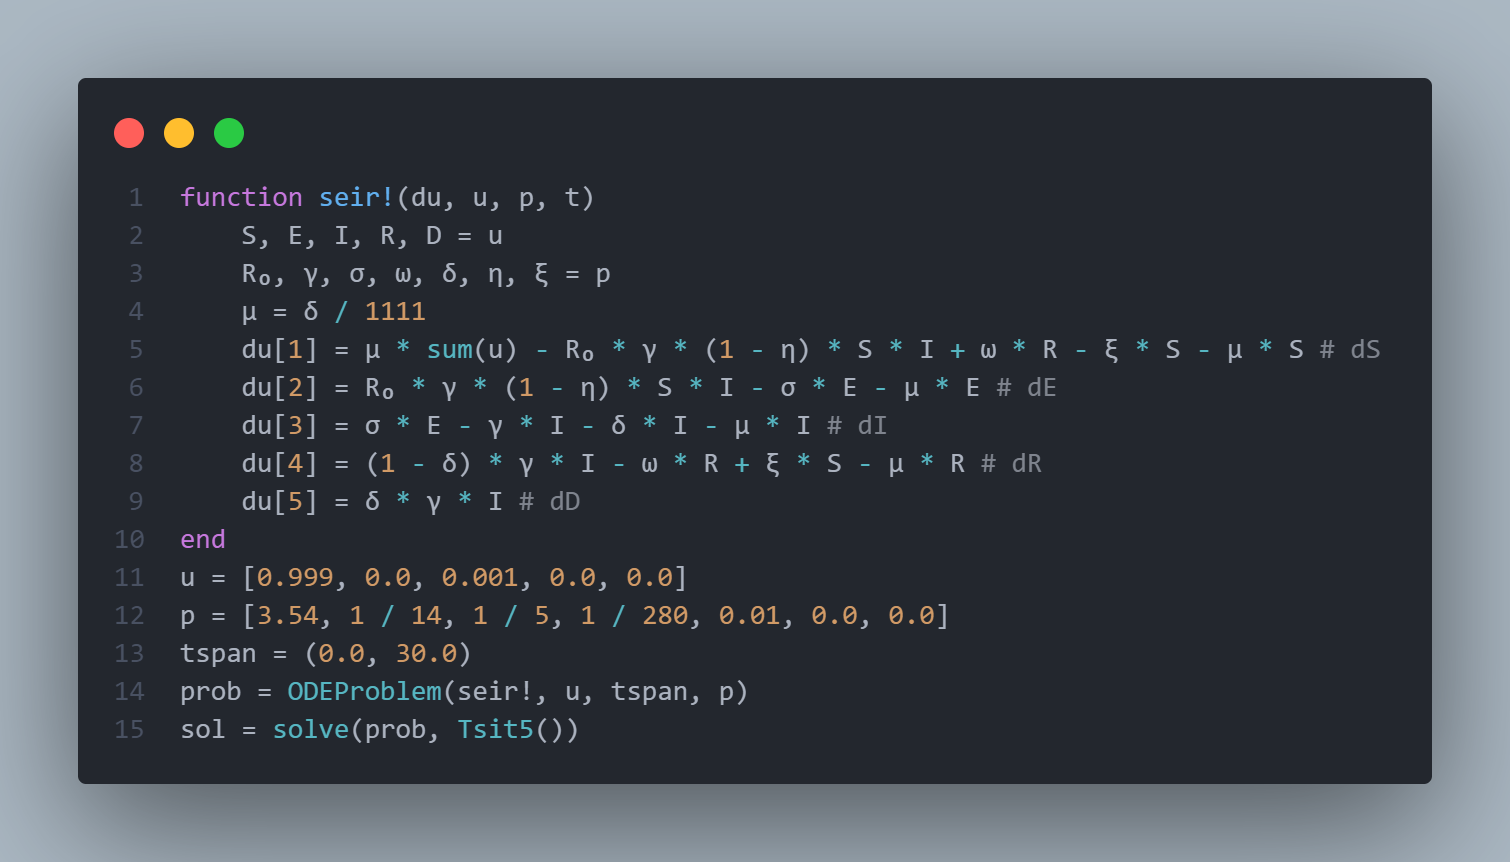
\includegraphics[width=\textwidth]{img/fdefinition.png}
        \caption{Esempio definizione ODE in Julia}
        \label{fig:ODE_Julia_example}
    \end{center}
\end{figure}

\subsubsection{Inserire un'ODE all'interno di una NN}

Per capire meglio cosa significhi inserire un'ODE all'interno di una 
rete neurale (NN), è necessario esaminare come è definito un layer di 
una NN. Un layer è essenzialmente una funzione differenziabile che 
accetta un vettore di dimensione $n$ come input e restituisce un nuovo 
vettore di dimensione $m$ come output. Questo si allinea con l'idea che 
i risolutori di DE rientrano nella categoria delle funzioni 
differenziabili, il che significa che possono essere incorporati 
direttamente in un programma più grande basato su differenziazione 
automatica, come una rete neurale \cite{Flux.jl-2018} \cite{pal2023lux}. 

Successivamente, è possibile addestrare la NN per un numero specifico di 
integrazioni per ottenere i risultati desiderati. È importante 
sottolineare che il sistema non sta apprendendo una soluzione 
all'equazione differenziale, ma piuttosto sta apprendendo il sistema di 
equazioni differenziali da cui è generata la soluzione. La NN sta 
effettivamente apprendendo una rappresentazione compatta del comportamento 
della serie di dati nel tempo e può estrapolare facilmente cosa 
potrebbe accadere con diverse condizioni iniziali. 

La suite DiffEqFlux.jl offre un wrapper comodo per definire una "NeuralODE" 
\cite{rackauckas2019diffeqflux}.

\begin{figure}[H]
    \begin{center}
        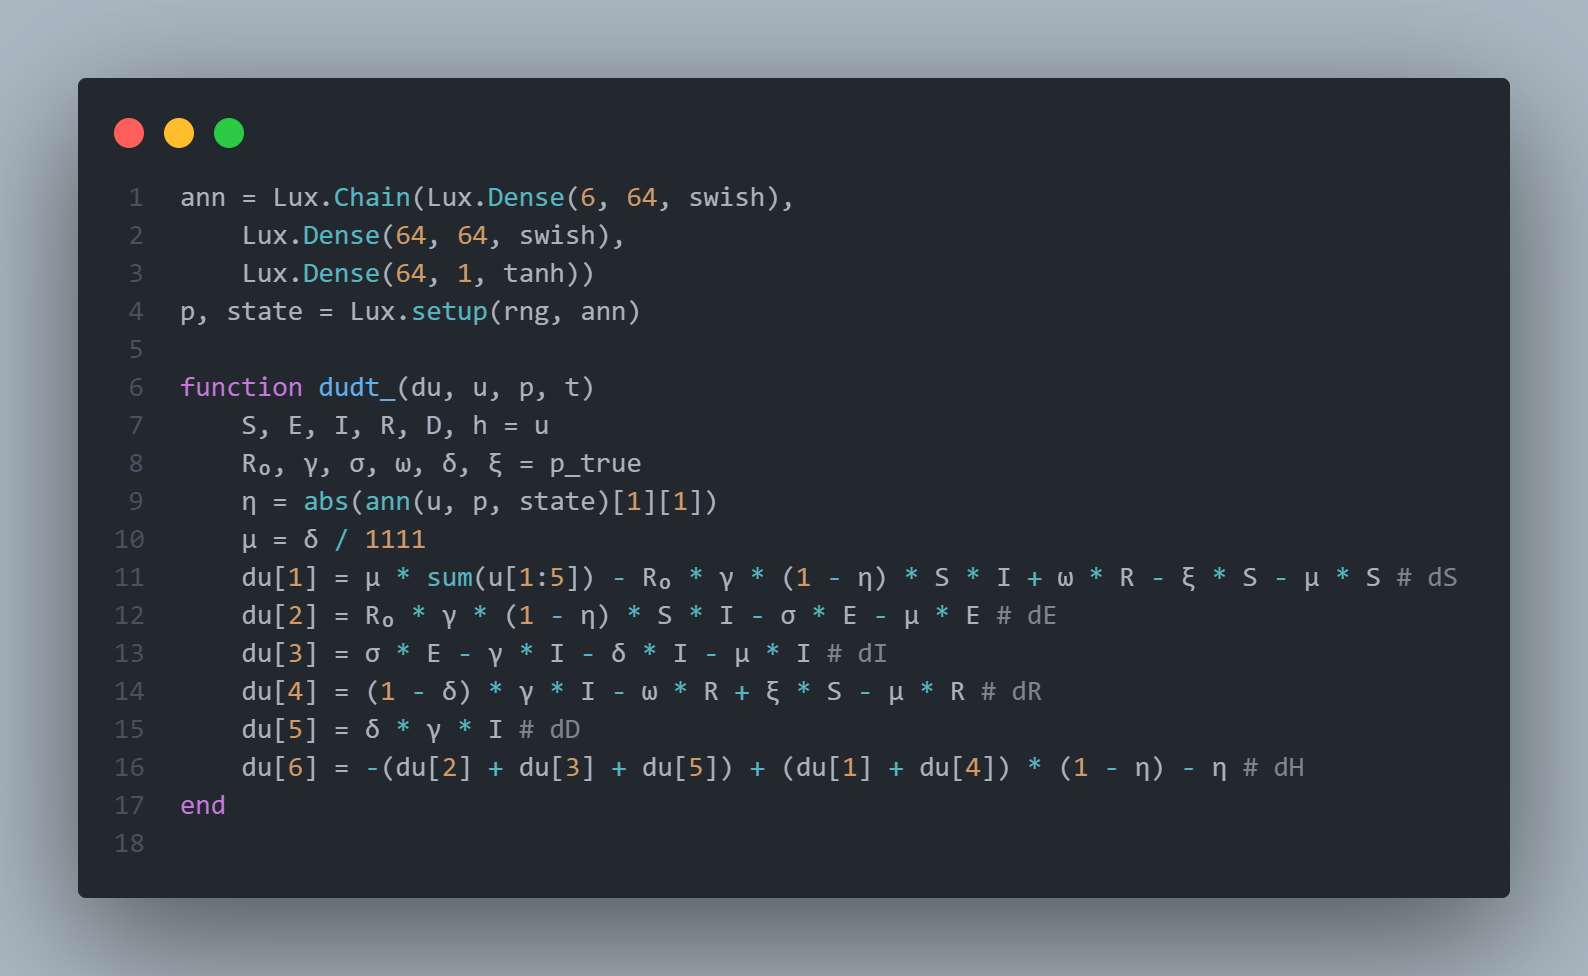
\includegraphics[width=\textwidth]{img/fann.png}
        \caption{Esempio implementazione di una rete neurale in Julia}
        \label{fig:NN_Julia_example}
    \end{center}
\end{figure}

\subsubsection{Backpropagation tramite ODE solver}

Il cuore di ogni rete neurale è la capacità di propagare all'indietro 
le derivate lungo l'intera rete per calcolare il gradiente della 
funzione di perdita rispetto ai parametri della rete. La sfida sta nel 
trovare un modo per applicare lo stesso principio quando si utilizzano 
risolutori di ODE all'interno di una rete neurale.

Esistono vari approcci per affrontare questo problema, ma il più comune 
è attraverso l'analisi di sensitività (adjointed). Questo approccio 
definisce una nuova ODE il cui obiettivo è calcolare il gradiente della 
funzione di costo rispetto ai parametri e successivamente risolvere 
questa seconda ODE.

L'approccio dell'analisi di sensitività (adjointed) comporta la 
definizione di una nuova ODE, chiamata anche "ODE aggiunta" o 
"ODE ausiliaria," il cui scopo principale è calcolare il gradiente 
della funzione di costo rispetto ai parametri della rete. 
Questa ODE ausiliaria è progettata in modo specifico per catturare 
come varia la funzione di costo al variare dei parametri, 
consentendo così il calcolo efficiente del gradiente.

Il processo può essere riassunto in modo generale nei seguenti passaggi:

\begin{itemize}
    \item \textbf{Forward Pass}: Durante la fase di forward pass 
    della rete neurale, vengono registrati i valori intermedi 
    necessari per risolvere l'ODE ausiliaria.
    \item \textbf{Calcolo della ODE Ausiliaria}: Durante la fase di 
    backward pass, la ODE ausiliaria viene risolta. 
    Questa ODE tiene conto dei valori intermedi registrati durante 
    il forward pass e calcola il gradiente della funzione di costo 
    rispetto ai parametri.
    \item \textbf{Backward Pass}: Il gradiente calcolato dalla ODE 
    ausiliaria viene quindi utilizzato per aggiornare i parametri 
    della rete neurale durante la fase di backward pass, consentendo 
    l'addestramento della rete mediante la discesa del gradiente.
\end{itemize}

Questo approccio è potente perché consente di calcolare il gradiente 
in modo efficiente anche quando sono presenti risolutori di ODE 
all'interno della rete. È uno strumento fondamentale nella progettazione 
e nell'addestramento di reti neurali che includono componenti basate 
su ODE, come le reti neurali differenziali (DNN).

In generale, l'analisi di sensitività è un concetto cruciale per 
consentire l'addestramento efficiente di modelli complessi e ibridi 
che combinano reti neurali con risoluzione di ODE o altre funzioni non 
lineari.

% descrizione dei metodi, strumenti e approcci utilizzati
\section{Metodi e Modelli}

\subsection{Modello ad Agente}
L'approccio utilizzato e' stato quello di modellare l'intero problema come 
se fosse una \emph{rete sociale}. L'idea e' nata tramite dopo aver osservato e 
studiato attentamente il problema proposto. 

Il problema si presenta come lo studio della diffusione di una pandemia a trasmissione
virale in un ambiente reale, il quale e' composto principalmente di cosi' detti 
\emph{Punti di Interesse} (PdI). Questi punti di interesse successivamente sono 
collegati tra loro tramite una rete piu' o meno fitta di collegamenti. Questa costruzione
ricorda in maniera molto stretta una struttura dati largamente utilizzata, ovvero il \textbf{Grafo}.

Con questo approccio la modellazione del problema e soprattutto la dinamica intera del 
modello verte piu' su un approccio di tipo \emph{mesoscopico} tendente al \emph{macroscopico}.
Questo poiche' per quanto l'idea di modellare un sistema ad agente estremamente granulare fosse 
di non poco interesse, al lato pratico ci si sarebbe scontrati con delle difficolta' 
intrinseche ad una modellazione cosi' specifica, la quale non si adattava all'idea piu' 
ampia del problema. Difatti non si vuole modellare un sistema a livello microscopico per vedere
le possibili interazioni tra agenti differenti, bensi' si vuole vedere la risposta collettiva di un
agente astratto all'utilizzo di interventi mirati e specifici per contrastare l'epidemia in 
maniera localizzata.

% immagine grafo
\subsubsection*{Approccio con Rete Sociale}
Il modello utilizzato sfrutta una proprieta' del framework \textbf{Agents.jl} e definisce un 
modello ad agente di tipo \textbf{ABM}. Essendo che in questo caso la struttura spaziale non 
del modello non e' importante ma le sue connessioni si, vengono definiti gli agenti come nodi
veri e propri del grafo in cui al loro interno viene simulato il ciclo di vita della pandemia 
tramite un modello di tipo \textbf{SEIR} deterministico.

\begin{minipage}{\linewidth}
    \centering
    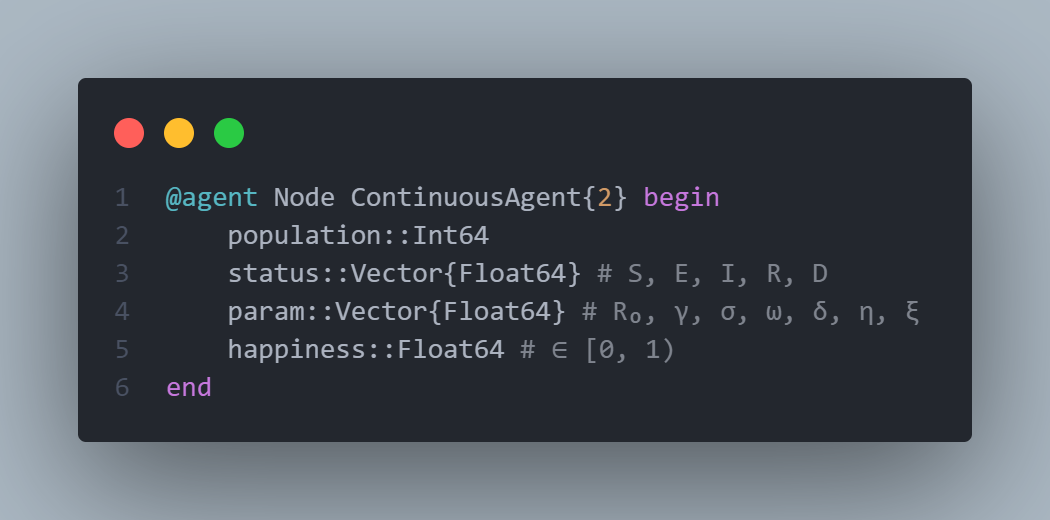
\includegraphics[width=\textwidth]{img/node_agent.png}
    \captionof{figure}{Codice Agente}
    \label{fig:Agent_code}
\end{minipage}

La struttura dell'agente e' di tipo \textbf{ContinuousAgent} in quanto lo 
spazio del modello e' di tipo continuo. Questa scelta e' stata fatta in vista di possibili 
sviluppi futuri dell'applicazione.

Successivamente si puo' osservare come il modello generato sia molto snello,
avendo solamente una manciata di parametri sufficienti al corretto funzionamento 
del modello stesso, senza risultare confusionari. 

\begin{minipage}{\linewidth}
    \centering
    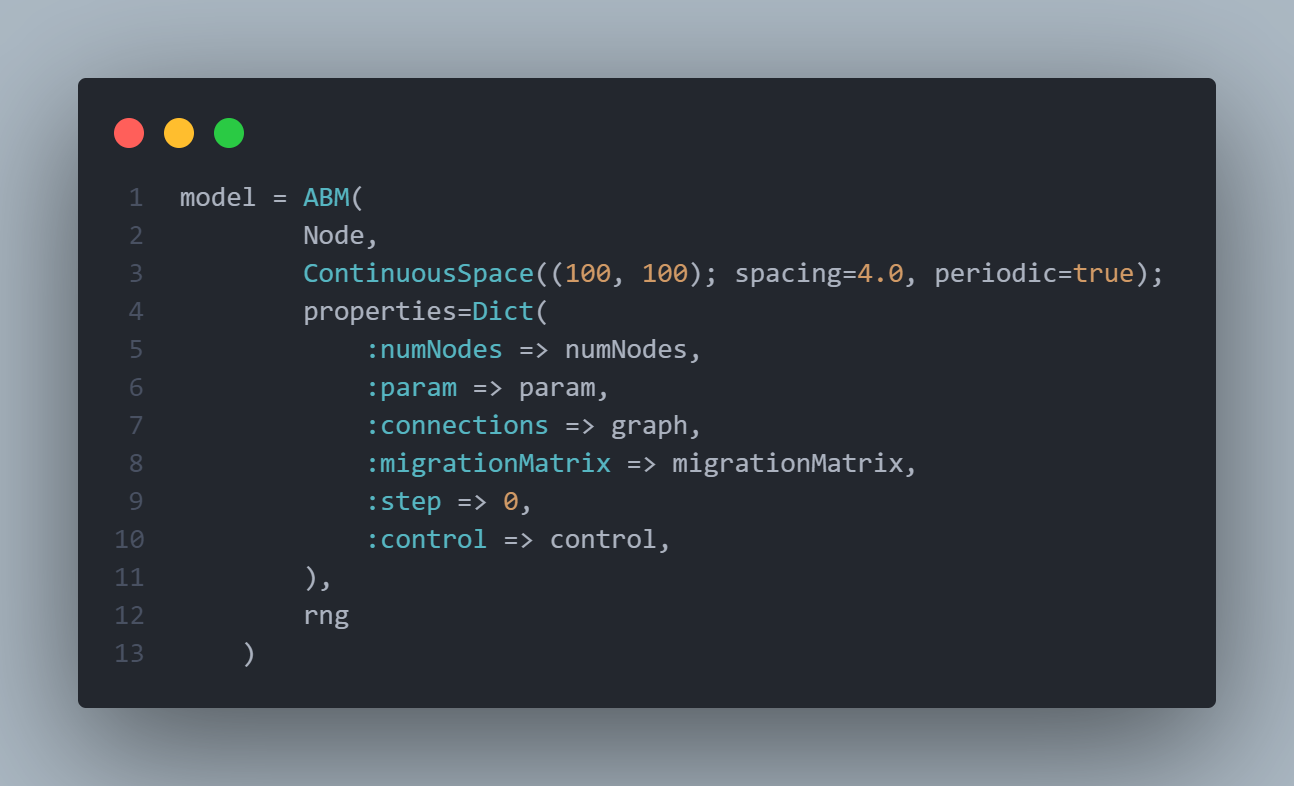
\includegraphics[width=\textwidth]{img/sngraph_model.png}
    \captionof{figure}{Codice Modello}
    \label{fig:Model_code}
\end{minipage}

\subsubsection*{Agente}
Come mostrato in figura \ref{fig:Agent_code} l'agente al suo interno e' molto minimale,
descrivendo solamente gli attributi necessari e sufficienti per la corretta modellazione
e interazione con se stesso. L'evoluzione di ogni agente e' completamente indipendente 
anche se questa puo' essere influenzata da altri agenti della rete, modificando l'altrimenti 
determinismo del modello SEIR al suo interno. 

I campi principali dell'agente sono i seguenti:
\begin{itemize}
	\item \textbf{population}: questo campo descrive tramite un valore di tipo \textbf{Int}
	il numero totale di individui che ad ogni step del modello si trovano all'interno di uno 
	specifico nodo. 
	\item \textbf{status}: questo campo descrive tramite un vettore di tipo \textbf{Flaot64}
	lo stato della popolazione all'interno del nodo. Questo stato viene descritto come 
	percentuale di individui, per cui i valori all'interno del vettore saranno tutti compresi 
	tra 0 e 1. La scelta di utilizzare questo approccio e' nata principalmente per motivi di 
	\emph{type stability} in quanto le operazioni di risoluzione del sistema di ODE altrimenti 
	potrebbero risentirne. Tuttavia e' stato fatto anche per un fattore di \emph{facilita' di comprensione}.
	\item \textbf{param}: questo campo descrive tramite un vettore di tipo \textbf{Float64}
	il parametro del modello SEIR specifici del nodo in questione. Questi parametri sono comprensivi 
	non solo dei valori relativi all'epidemia, ma anche dei valori relativi alle contromisure, 
	in particolare le contromisure \textbf{non farmaceutiche} e quelle \textbf{farmaceutiche}.
	\item \textbf{happiness}: questo campo e' utilizzato come campo di appoggio per il bilanciamento
	delle contromisure applicate dal controllore. Non esprime effettivamente la misura della felicita'
	che la popolazione di un nodo ha complessivamente, ma e' comunque uno stimatore similare.
\end{itemize}

\subsubsection*{Spazio e Modello}
Come accennato precedentemente e mostrato in figura \ref{fig:Model_code}, lo spazio del modello 
e' di tipo \textbf{ContinuousSpace} seppure non venga effettivamente sfruttato a dovere. 
Tuttavia l'interesse del modello e' il fatto che utilizzi una struttura come un grafo in maniera
astratta per modellare le interazioni tra i suoi nodi, ovvero gli agenti, in maniera rapida e efficente.

Per prima cosa viene creato il modello tramite la creazione di un grafo \emph{connesso}, il cui 
numero di archi dipende da quanto l'utente vuole che siano connessi i nodi. Piu' alto e' il 
desiderio di copertura piu' archi verranno creati. Tuttavia ci sono dei limiti superiori e inferiori 
sul numero di nodi creabili.

Il grafo che si va a creare e' \emph{non orientato}, per cui il numero minimo di archi necessari 
per costruire un grafo connesso, ovvero un grafo in cui da ogni nodo e' sempre possibile raggiungere
tutti gli altri nodi tramite un percorso che li collega, diventa il segunte, $numEdges = numNodes-1$
e questo pone il limite inferiore. Quello superiore e' dato dalla costruzione di un grafo completo, 
un grafo per cui ogni nodo e' collegato con tutti gli altri nodi appartenenti al grafo. In questo 
caso il numero di archi necessari e': $numEdges = \frac{numNodes*(numNodes-1)}{2}$.

All'interno di questi due limiti, viene creato il grafo secondo le esigenze dell'utente.

\begin{figure}[!hb]
	\centering
	\begin{subfigure}[b]{0.45\textwidth}
		\centering
		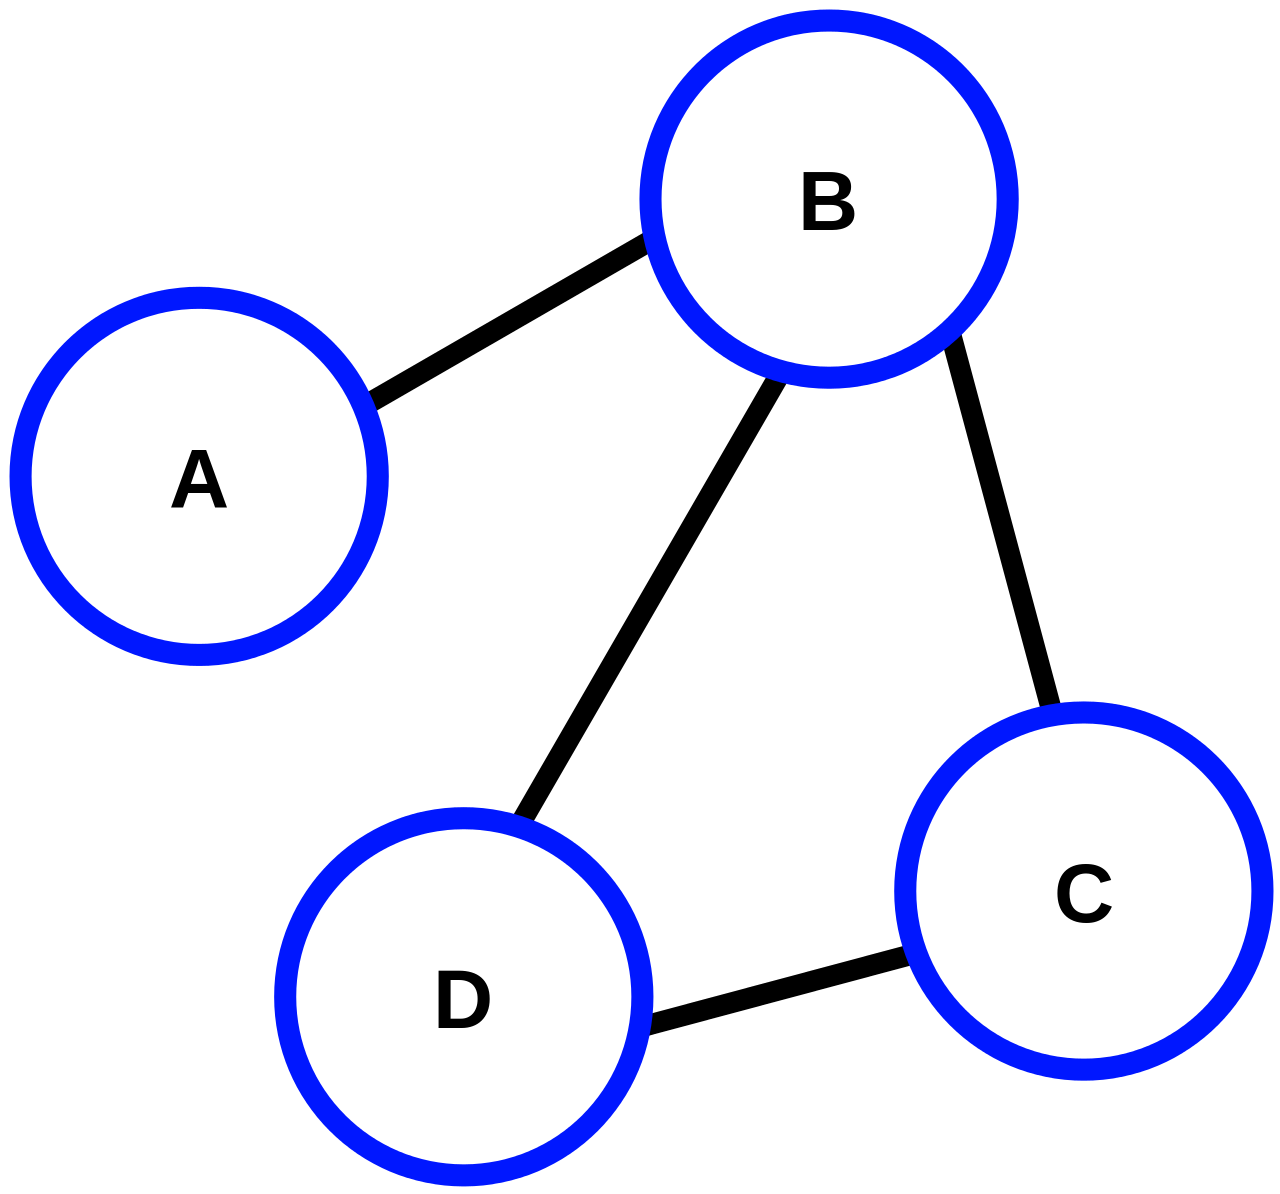
\includegraphics[width=\textwidth]{img/CPT-Graphs-undirected-unweighted-ex1.svg.png}
		\caption{Esempio di grafo connesso}
		\label{fig:connected_graph_example}
	\end{subfigure}
	\hfill
	\begin{subfigure}[b]{0.45\textwidth}
		\centering
		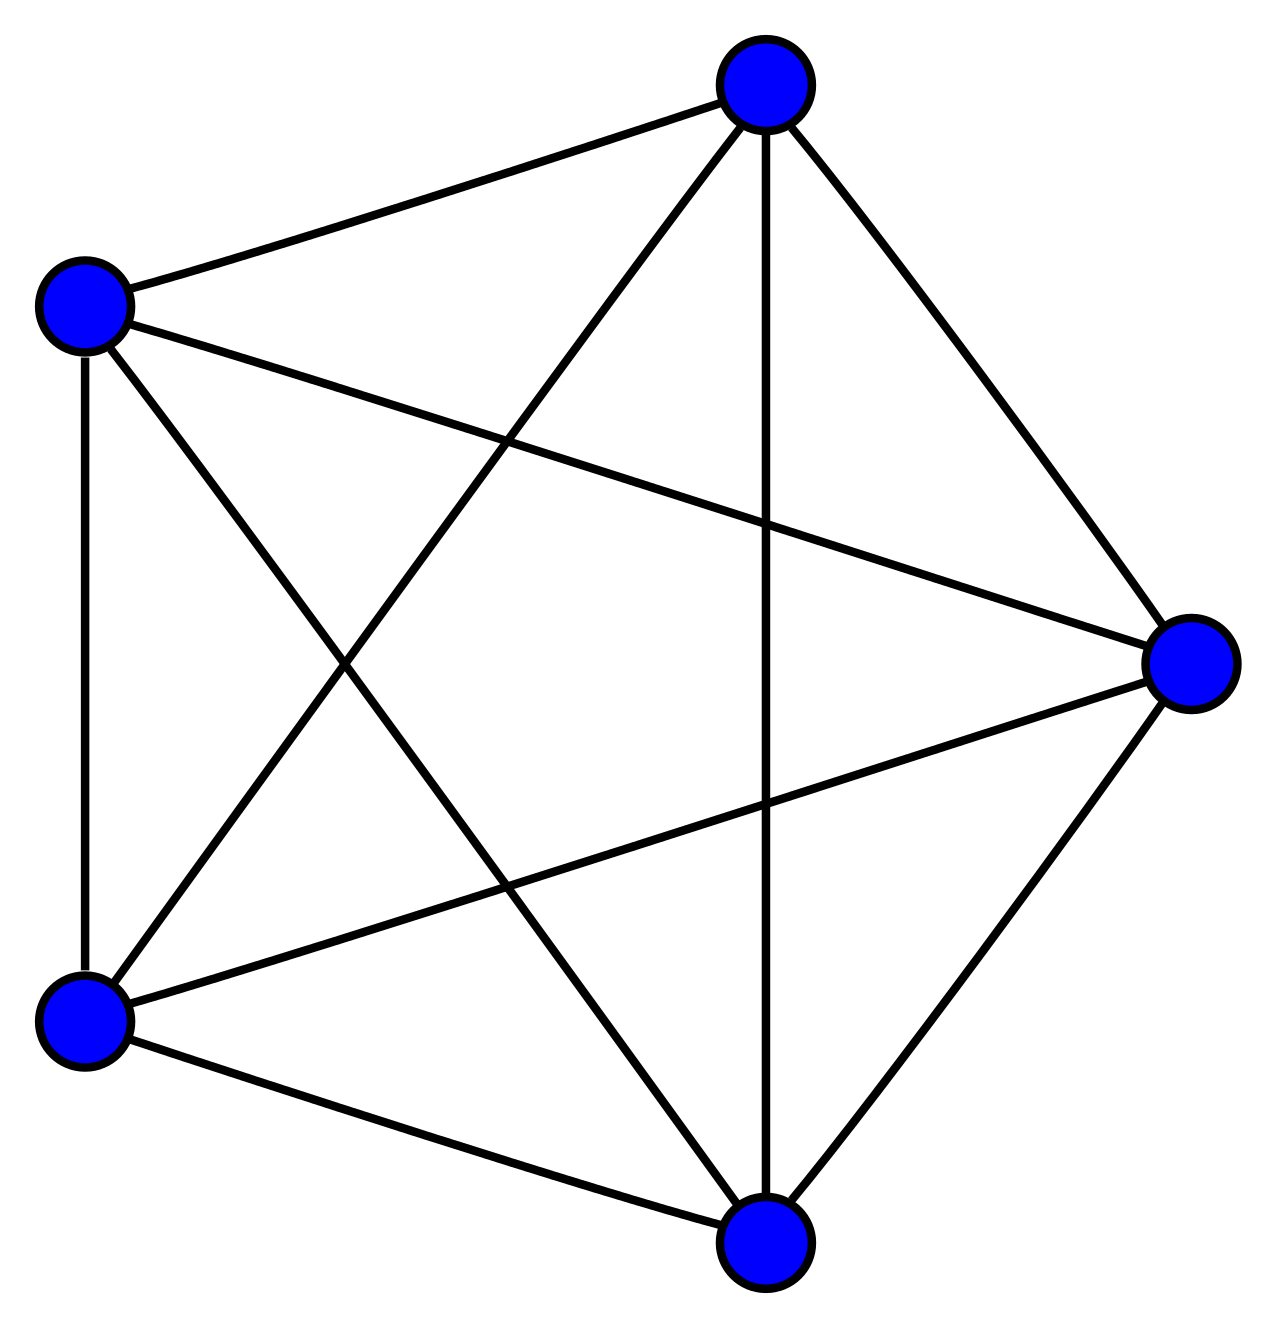
\includegraphics[width=\textwidth]{img/4-simplex_graph.svg.png}
		\caption{Esempio di grafo completo}
		\label{fig:complete_graph_example}
	\end{subfigure}
\end{figure}

Successivamente viene creata una matrice di flusso, denominata come \textbf{migrationMatrix}
che rappresenta la percentuale di individui che dal nodo di interesse si spostano verso 
un nodo di destinazione. Questa matrice e' salvata come \textbf{matrice sparsa} per risparmiare
spazio dove le connessione non sono presenti tra i nodi. 

\begin{minipage}{\linewidth}
	\centering
	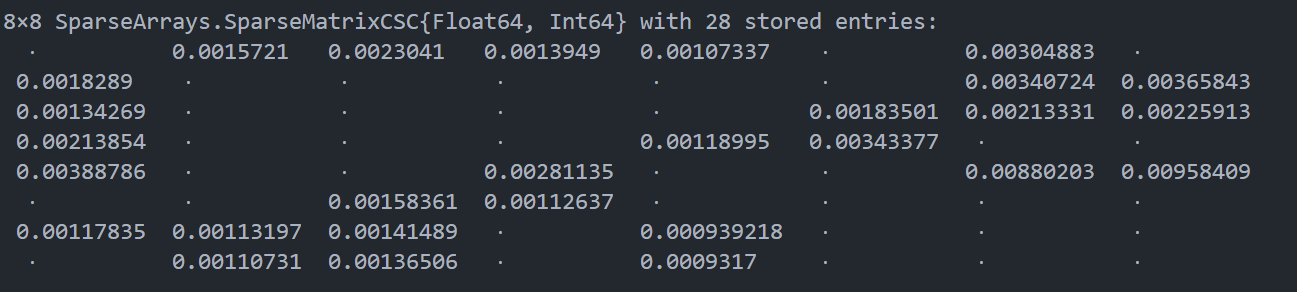
\includegraphics[width=\textwidth]{img/migrationMatrix.png}
	\captionof{figure}{Matrice di migrazione}
	\label{fig:migration matrix}
\end{minipage}

Questa matrice viene esplicitamente creata in base alla topologia del grafo che viene 
inizializzato in precedenza e si occupa di pesare gli archi di quest'ultimo seguendo la 
filosofia per cui si ha un flusso maggiore verso i nodi piu' popolosi, e minore verso i 
nodi meno popolosi. Questo flusso ha poi un limite massimo che puo' essere scelto e 
modificato dall'utente. 

Se questa matrice fosse una matrice non sparsa, e percio' completa, si potrebbe osservare
come la diagonale di questa matrice ha valori molto vicini ad 1, in relazione con il limite
massimo di individui che possono migrare da ogni nodo, definito come \emph{migration rate}.

Successivamente, dopo avere popolato ogni agente (o nodo) del modello con i corretti valori,
dato che la struttura interna su cui viene effettuata la computazione del modello e' basata su 
un sistema di ODE, viene istanziato un array di \textbf{ODEProblem}. L'idea di spezzettare
un sistema di ODE in piu' sottosistemi di ODE collegate tra loro tramite uno scambio continuo 
di informazioni (in questo caso individui), e' stata pubblicata nel seguente articolo \cite{Ding2021}
in cui si modella l'outbreak da COVID-19 tenendo in considerazione il flusso migratorio 
dei voli aerei. 

Applicando tale filosofia, e' possibile creare un array di \textbf{ODEProblem}, oggetti che descrivono
un sistema di equazioni differenziali ordinarie, ai quali viene messo a corredo un \textbf{integratore}. 
Quest'ultimo fa le veci della classica funzione \textbf{solve} che si occupa di risolvere l'intero sistema.

\begin{minipage}{\linewidth}
	\centering
	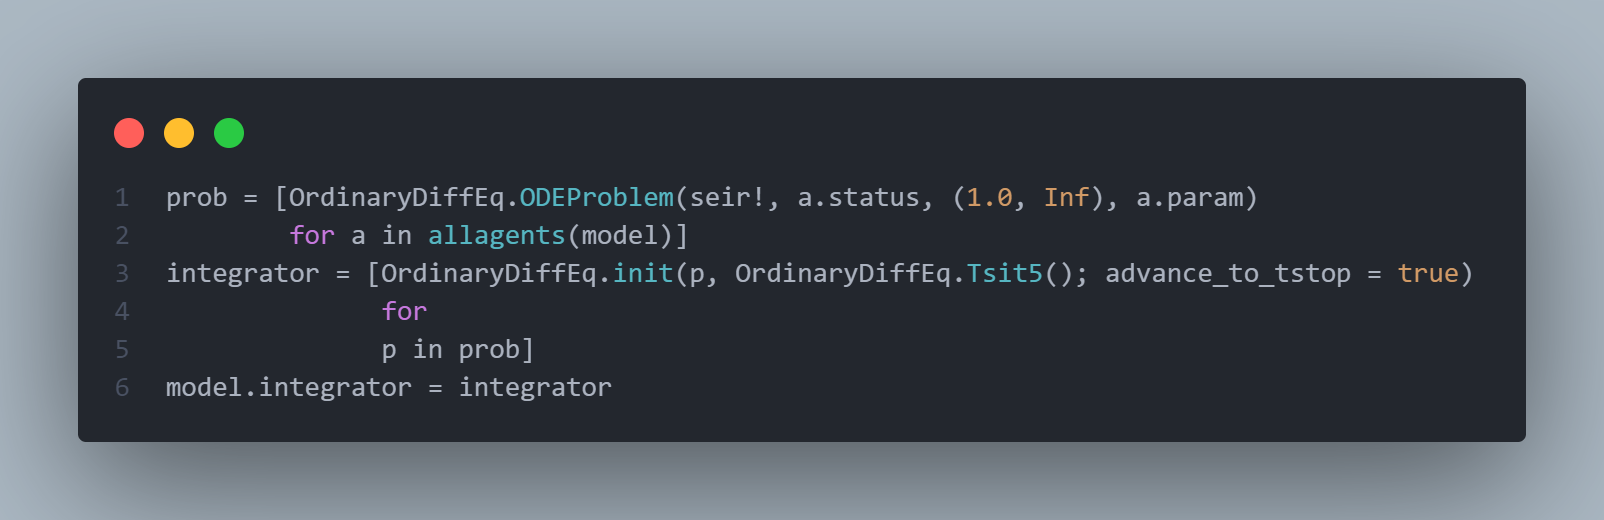
\includegraphics[width=\textwidth]{img/model_ode.png}
	\captionof{figure}{Definizione dei sistemi di ODE associati ad ogni agente}
	\label{fig:model_ode}
\end{minipage}

L'approccio scelto, ovvero di usare un integratore, puo' essere sostituito tramite
l'uso di funzioni di \textbf{callback} le quali permettono quando vengono soddisfatte delle
condizioni di attivazione specifiche, di andare a modificare i parametri del sistema che
si sta risolvendo. Queste modifiche tuttavia, possono portare delle discontinuita' nella 
risoluzione, ma queste vengono esplicitamente gestite se viene specificata una funzione 
di callback all'interno della funzione di solve. 

I due approcci sono completamente equivalenti e la scelta di uno piuttosto che dell'altro
ricade solamente su un fattore di comodita' d'uso.

\subsubsection*{Funzione di avanzamento agente}
Un agente finche' all'interno di un modello segue ciclicamente il comportamento
riportato in figura \ref{fig:agent_behaviour}

\begin{minipage}{\linewidth}
	\centering
	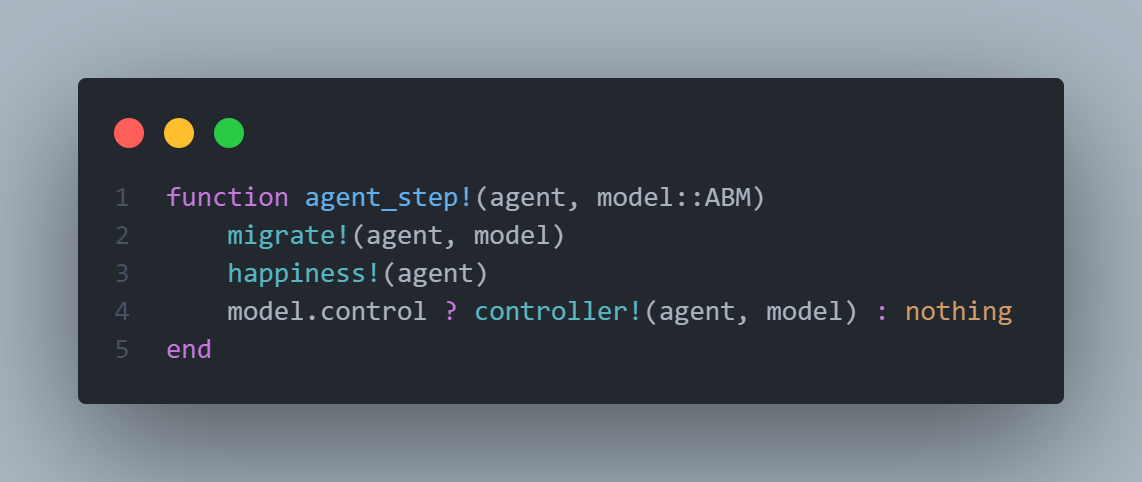
\includegraphics[width=\textwidth]{img/agent_behaviour.png}
	\captionof{figure}{Comportamento agente}
	\label{fig:agent_behaviour}
\end{minipage}

Ad ogni passo del modello, vengono attivati tutti gli agenti presenti al suo interno e 
fatti aggiornare seguendo le regole di scheduling preposte. 

Ad ogni passo, un agente e' chiamato ad eseguire tre fondamentali compiti:
\begin{itemize}
	\item \textbf{Muoversi}: un agente come entita' essendo un nodo di un grafo non puo'
	muoversi nel modo piu' letterale del termine, ma tramite la sua matrice di migrazione 
	e' possibile calcolare quanti individui si spostano da il nodo sorgente, fino ad un nodo
	destinazione. Questo spostamento fa si che il nodo venga aggiornato con le relative percentuali
	di status e il totale di popolazione rimanente
	\item \textbf{Calcolare la felicita'}: come detto in apertura della sezione, il valroe di \textbf{happiness}
	e' un valore fantoccio che serve prevalentemente per bilanciare le contromisure del controllore.
	Questo valore tuttavia viene influenzato anche dalla situazione pandemica. Attualmente la funzione che si occupa di generare la felicita' complessiva di un nodo si basa
	sull'utilizzo di una \emph{tangente iperbolica} (tanh) che prende come parametro il valore attuale
	di happiness del nodo e lo bilancia con il valore delle contromisure $\eta$ associate e attualmente 
	uso. Questo approccio e' sicuramente problematico e fallace per numerosi motivi ma attualmente 
	adempie al suo obiettivo.
	\item \textbf{Chiamare un controllore}: se la proprieta' \emph{control} del modello e' impostata su
	\emph{true}, viene chiamato il controllore che si occupa di stimare, data la situazione attuale del nodo
	quanto stringenti devono essere le policy da applicare al nodo in questione, andando ad utilizzare
	un insieme di tecniche di ottimizzazione non lineare ottenuta dalla suite \textbf{Ipopt} per 
	stimare quale dovrebbe essere la policy migliore da applicare dato un valore massimo di costo.
\end{itemize}

\subsubsection*{Funzione di avanzamento modello}
Ogni passo di avanzamento del modello segna un passo di avanzamento dell'intero sistema. 
Questo vuol dire che all'interno di un passo del modello vi e' un passo per ogni agente. Di default
il framework Agents.jl effettua prima l'avanzamento degli agenti e successivamente quello del modello.
Questo comportamento puo' essere modificato quando viene chiamata la funzione di \textbf{step!} che 
si occupa di far girare l'intero sistema.

Il modello si occupa ad ogni passo di effettuare tutte quelle operazioni che non sono legate ad un
singolo agente ma che sono legate o alla comunita' di agenti oppure al modello in quanto sistema complesso. 

\begin{minipage}{\linewidth}
	\centering
	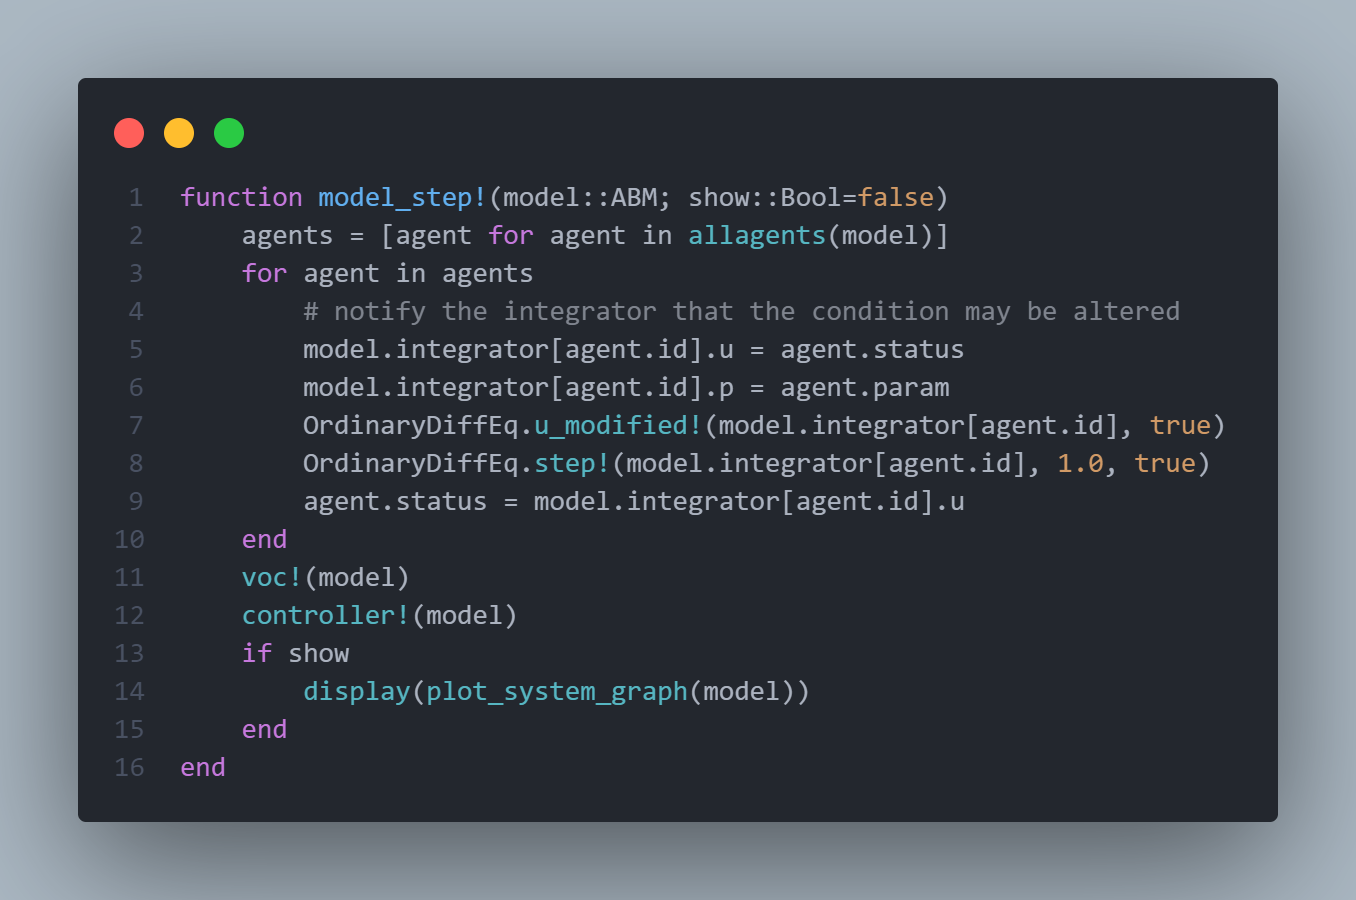
\includegraphics[width=\textwidth]{img/model_step.png}
	\captionof{figure}{Funzione di avanzamento del modello}
	\label{fig:model_step}
\end{minipage}

Come e' possibile osservare dalla figura \ref{fig:model_step}, il sistema si occupa principalmente
di aggiornare notificare l'integratore di ogni agente e aggiornarlo indicandogli che le condizioni
precedenti possono essere state alterate, e successivamente effettuare un passo del sistema di 
integrazione. Successivamente il modello si preoccupa di generare una nuova \emph{Variant of Concern} (VOC)
e infine di chiamare la funzione \textbf{vaccine!} la quale e' responsabile del calcolo e dell'applicazione 
delle misure di contromisure farmaceutiche all'interno della popolazione. 

Questa sezione e' quella che piu' presta il fianco ad \emph{assunzioni} riguardo 
il comportamento generale del sistema. Tutte le funzioni sopra descritte si basano su un insieme
piu' o meno nutrito di assunzioni per funzionare correttamente. Questo perche' al momento in cui sto 
redigendo questo documento \today, non sono ancora riuscito ad implementare metodi migliori. 

La funzione che si occupa di generare la \emph{variant of concern} (VOC) e' la seguente

\begin{minipage}{\linewidth}
	\centering
	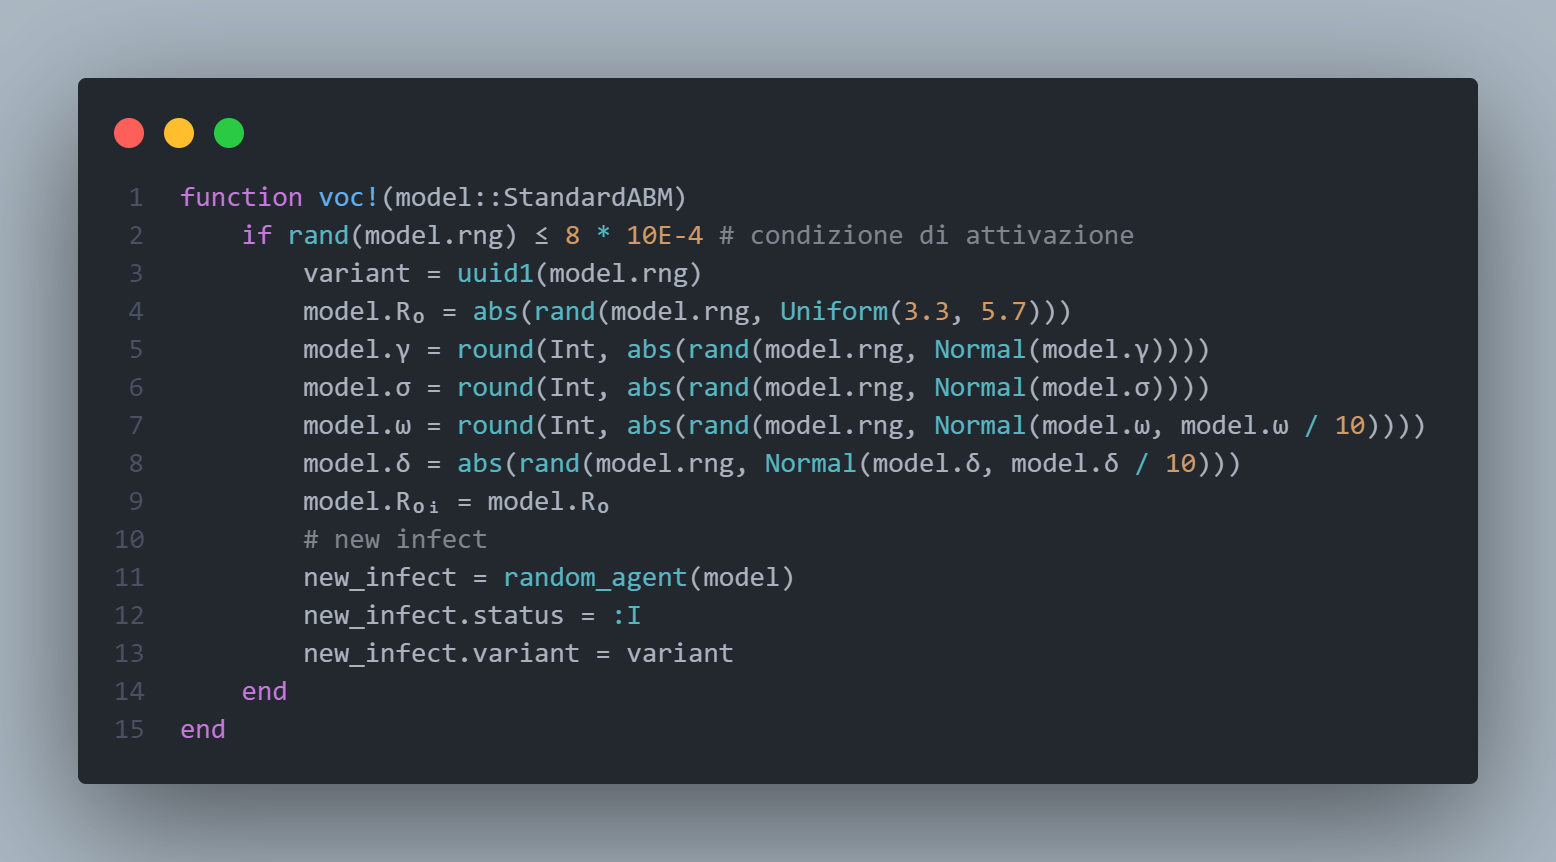
\includegraphics[width=\textwidth]{img/voc.png}
	\captionof{figure}{Funzione che si occupa di generare la VOC}
	\label{fig:voc}
\end{minipage}

Si possono notare molte assunzioni:
\begin{itemize}
	\item la condizione di attivazione della funzione si basa su un valore
	che sembra totalmente randomico. Quel valore, ovvero $8 \cdot 10e-4$ deriva dai
	seguenti articoli \cite{Markov2023} \cite{https://doi.org/10.1002/jmv.27331} \cite{Abavisani2022}
	i quali descrivono prevalentemente il tasso di mutazione casuale delle basi che compongono
	il DNA del virus SARS-COV2. Questo pero' non implica che tali mutazioni 
	creino una VOC. Per semplicita' e' stato scelto di usare l'approccio per cui
	se una mutazione avviene, questa e' un a VOC. In linea di massima sembra che 
	questo approccio semplicistico crei un numero di VOC generalmente sensato e 
	in linea con quanto abbiamo potuto osservare durante la pandemia
	\item la distribuzione dei parametri associati alla pandemia viene calcolata
	seguendo una distribuzione \textbf{Normale}, tranne per la distribuzione dell'indice $R_0$
	il quale segue una distribuzione di tipo \textbf{Uniforme} \cite{wiki:Numero_di_riproduzione_di_base}
\end{itemize}

La funzione che si occupa di stimare l'applicazione delle contromisure farmaceutiche, ovvero l'applicazione del vaccino,
e' la seguente, e anch'essa presta il fianco a numerevoli assunzioni, le quali pero' empiricamente parlando
effettuano una buona stima di come sono evolute le cose nel mondo reale.

\begin{minipage}{\linewidth}
	\centering
	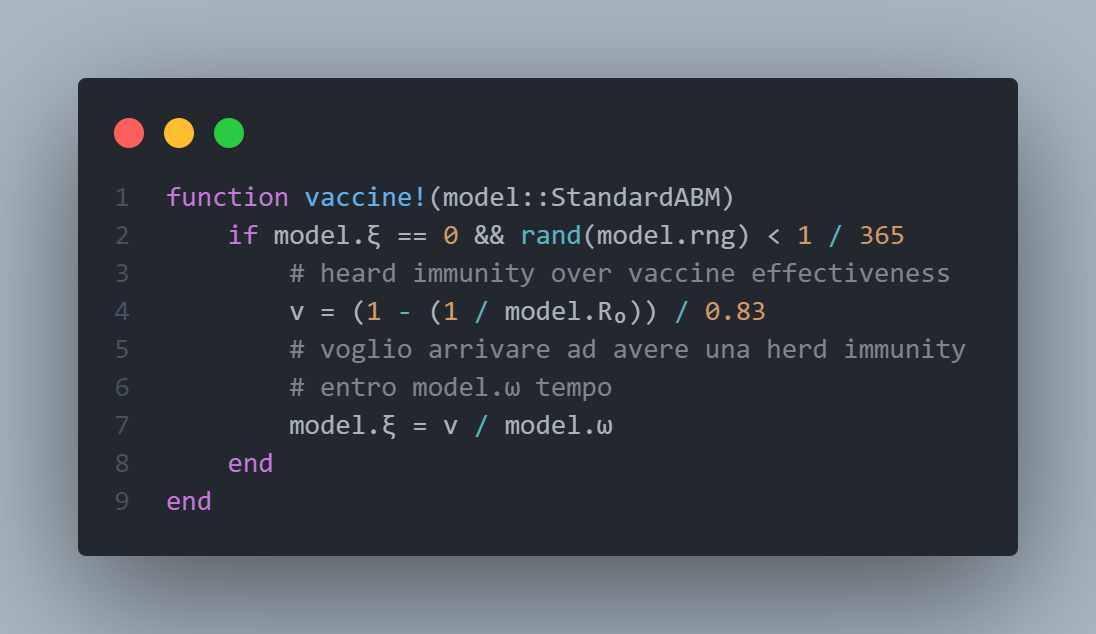
\includegraphics[width=\textwidth]{img/vaccine.png}
	\captionof{figure}{Funzione che si occupa di simulare la ricerca di un vaccino e la sua successiva applicazoine}
	\label{fig:vaccine}
\end{minipage}

Si nota come in generale la funzione si basa sul generare un valore fissato, generalmente $\in [0,1]$, che 
rappresenta la percentuale di popolazione che puo' essere vaccinata ad ogni passo del modello.
Questo approccio tende a simulare l'idea piu' o meno realistica di avere una quantita' fissata di 
dosi vaccinali ogni giorno che possono essere erogate alla popolazione. 

Questo calcolo viene effettuato tenendo in considerazione l'approccio dell' \emph{immunita' vaccinale di gregge} che puo'
essere ottenuta seguendo la formula 

$$V_c = \frac{1-\frac{1}{R_0}}{VaccineEfficiency}$$

Successivamente calcolo questo valore come un obiettivo da raggiungere entro un tempo $\omega$ che equivale al 
periodo di immunita' che un individuo ha dopo aver contratto la malattia (o aver effettuato il vaccino). 
Questa idea viene utilizzata per modellare le curve del modello in quanto un individuo vaccinato e' considerato 
come un individuo nello stato \emph{Recovered} e segue le stesse regole di chiunque altro, indipendentemente
dal modo in cui si e' entrati in questo stato. 

Questa visione semplicistica comunque e' efficace nel modellare il decorso di una malatti, con e senza interventi.

\subsubsection*{Grafico senza intervento}
Il seguente grafico \ref{fig:abm_no_intervent} mostra l'andamento delle curve del modello
quando questo viene eseguito senza alcuna tipologia di intervento. Questo andamento tuttavia e' mostrato 
in maniera cumulativa rispetto all'andamento dei singoli agenti, il quale puo' avere comportamentei 
differenti in base a se appare o meno una variante, come specificato in figura \ref{fig:voc}, oppure 
dipendentemente dal tipo di contromisure applicate. 

\begin{minipage}{\linewidth}
	\centering
	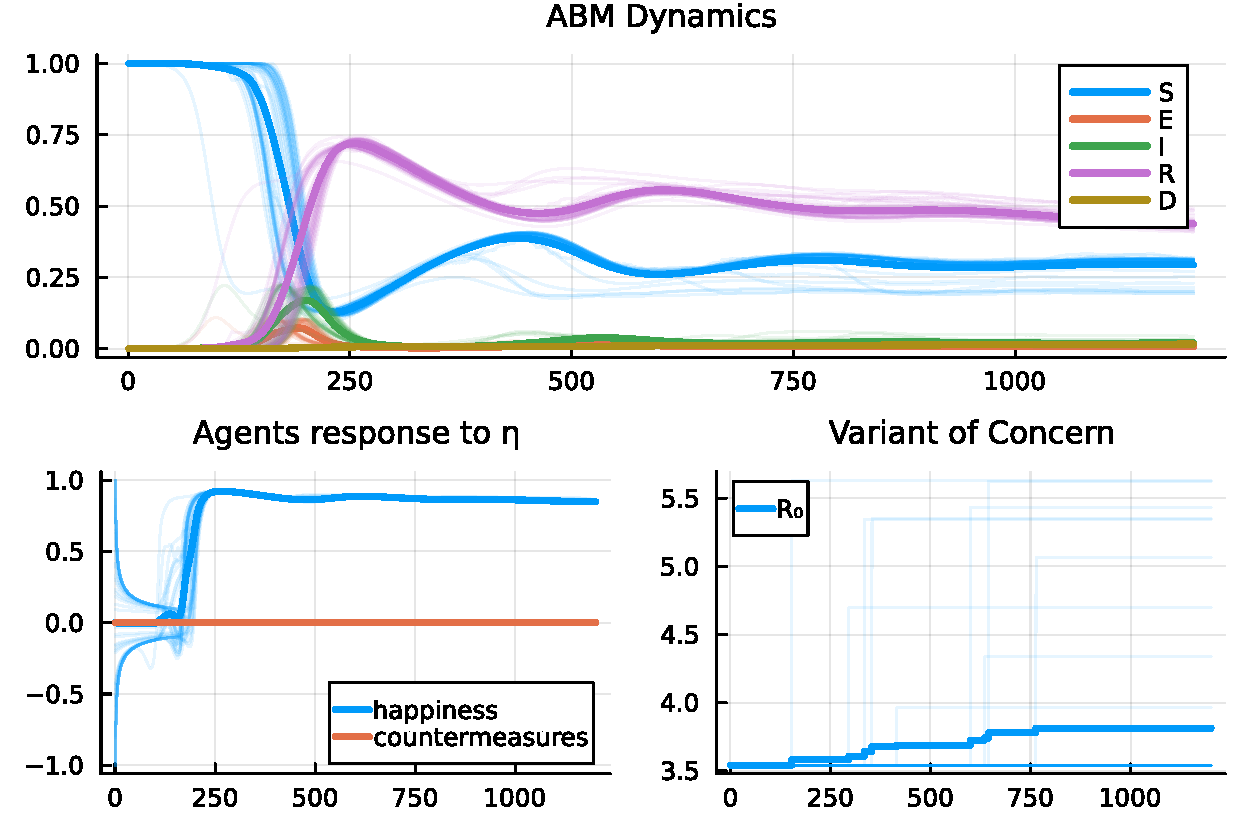
\includegraphics[width=\textwidth]{img/SocialNetworkABM_NO_CONTROL_2023-07-15.pdf}
	\captionof{figure}{Grafico cumulativo del risultato del modello senza intervento del controllore}
	\label{fig:abm_no_intervent}
\end{minipage}

Complessivamente pero' l'andamento e' ovviamente similare ad un andamento standard di un modello 
SEIR, con qualche variazione dipendente dai fattori di stocasticita' del modello che pero'
in questo caso non risultano troppo presenti, che vengono messi in evidenza con le curve del modello 
meno marcate, che rappresentano i percorsi "meno battuti" della simulazione.

Come e' possibile notare, il numero di individui suscettibili crolla drasticamente
per via della diffusione rapida e simil esponenziale che ha il virus. Questa viene emulata
dall'altrettanto rapida crescita di individui guariti (recovered) che pero', per via
di come e' stato definita la condizione di guariti, non sono immuni alle varianti del virus. 
Queste proprieta' contribuiscono ad un andamento ciclico delle curve, in particolar modo 
di quelle \emph{E, I, R}. La curva associata al compartimento \emph{S} ha un suo andamento
ciclico seppur molto sottile; questa sottigliezza e' dovuta all'assenza di misure di 
controllo all'interno del sistema.

Si puo' infine notare come la curva associata all'andamento degli individui
nella classe \emph{D} abbia una crescita lineare, seppur non troppo evidente.

A seguire si puo' osservare come la curva associata alla variabile di happiness del modello,
valore che serve per bilanciare la durezza delle misure di controllo per evitare 
di cadere in un ciclo funzionale ma insostenibile, mostra un comportamento alquanto bizzarro.
Questo e' dovuto principalmente a come viene definita la funzione di controllo della felicita' 
la quale essendo dominata principalmente da due fattori, $\eta$ ovvero le contromisure applicate
da un controllore e dalla proporzione tra il numero di individui nelle categorie \textbf{S, R} e 
gli individui nelle categorie \textbf{I, D} si arriva velocemente a comprenderne il funzionamento.
Si osserva inoltre che la curva tende ad un \emph{plateau} passato il periodo della "prima ondata". 

Questo comportamento e' irrealistico e associato alla definizione che e' stata fatta della 
funzione \textbf{happiness!}. Tuttavia anche se il comportamento di questa curva non e' 
completamente realistico, si puo' comunque utilizzare per mantenere sotto controllo le contromisure $\eta$.

Infine si nota come, seppur la definizione della funzione associata alla creazione di una
nuova \emph{Variant of Concern (VOC)} \ref{fig:voc} sia semplicistica e irrealistica, 
il grafico mostra come su un periodo di circa 3 anni, associabile alla durata del periodo covid, 
le voc sono al piu' una decina (ogni picco o depressione e' una voc). 

\begin{minipage}{\linewidth}
	\centering
	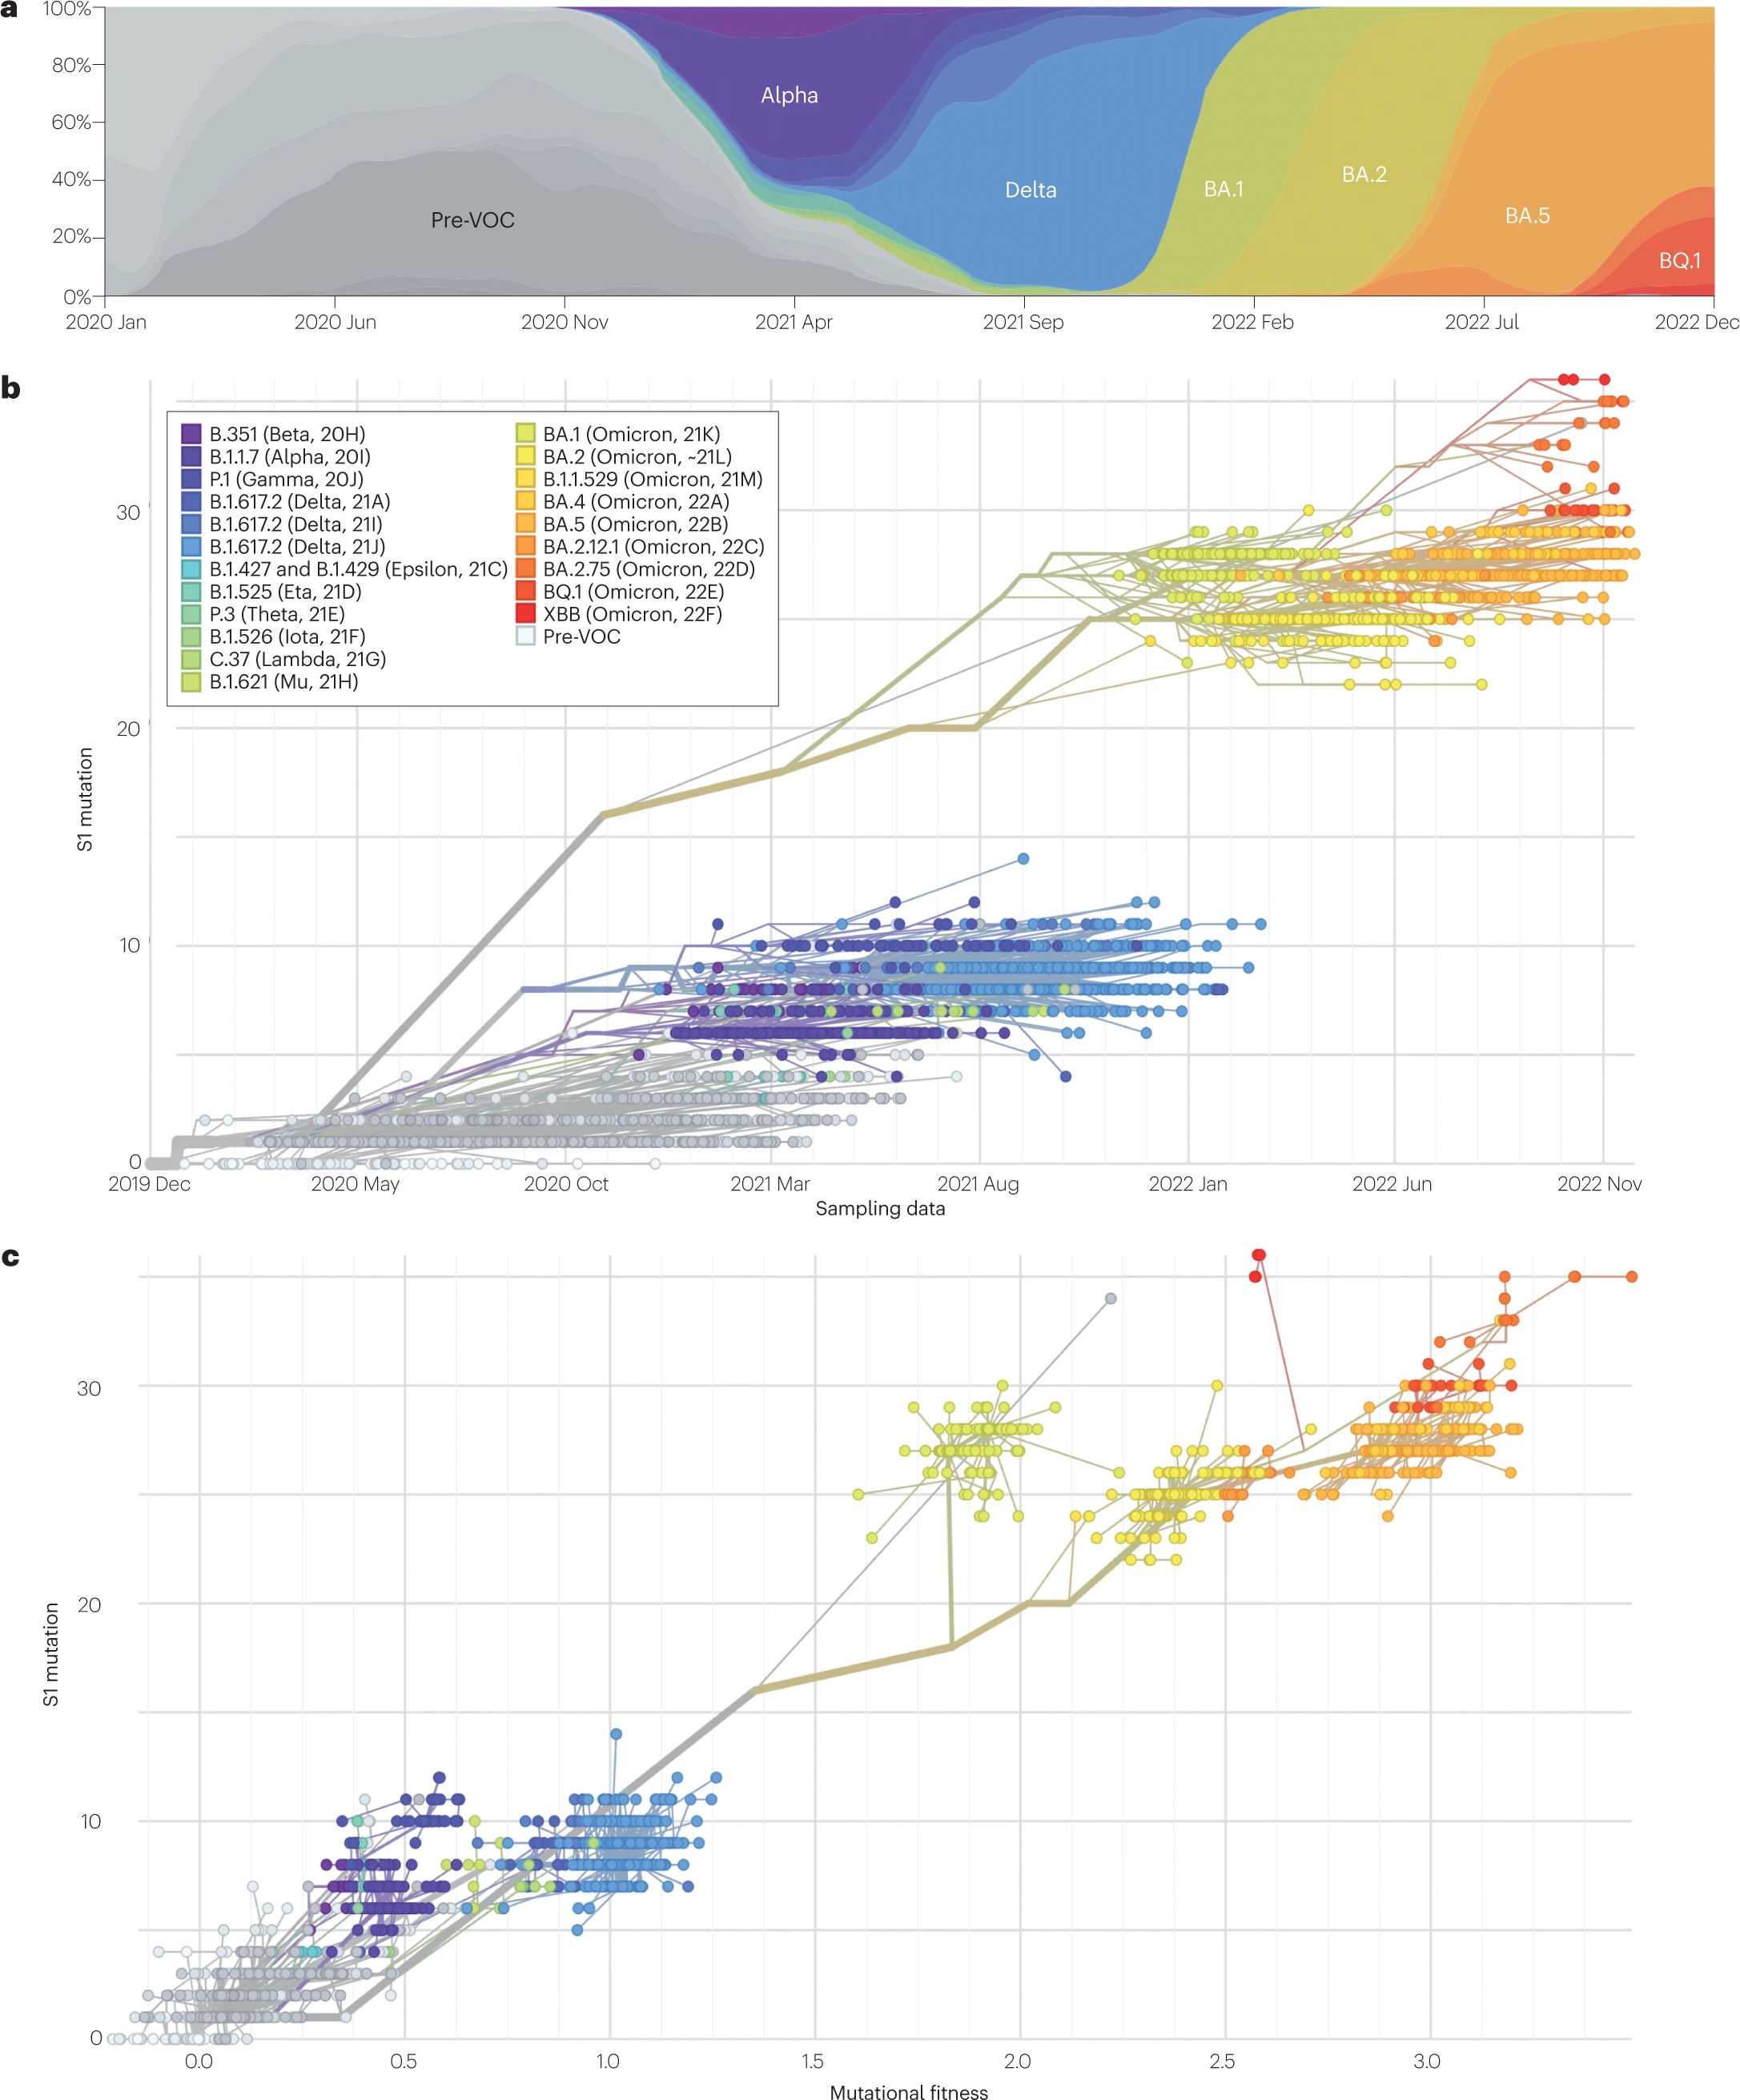
\includegraphics[scale=0.15]{img/41579_2023_878_Fig3_HTML.png}
	\captionof{figure}{Grafico delle mutazioni casuali del virus SARS-COV2 preso dall'articolo \cite{Markov2023}}
	\label{fig:covid_mutation}
\end{minipage}

Si nota come le voc scoperte del covid siano una quantita' pressoche' similare seppur con una 
distribuzione all'interno della linea temporale differente. Tuttavia il comportamento semplicistico 
applicato nel modello sembra essere una buona approssimazione del comportamento reale del virus.

\subsubsection*{Grafico con intervento}

Il seguente grafico \ref{fig:abm_intervent} mostra l'andamento delle curve del modello
quando questo viene eseguito tramite l'applicazione di una qualche tipologia di intervento. 
Questo andamento tuttavia e' mostrato in maniera cumulativa rispetto all'andamento dei singoli agenti, il quale puo' avere comportamentei 
differenti in base a se appare o meno una variante, come specificato in figura \ref{fig:voc}, oppure 
dipendentemente dal tipo di contromisure applicate. 

\begin{minipage}{\linewidth}
	\centering
	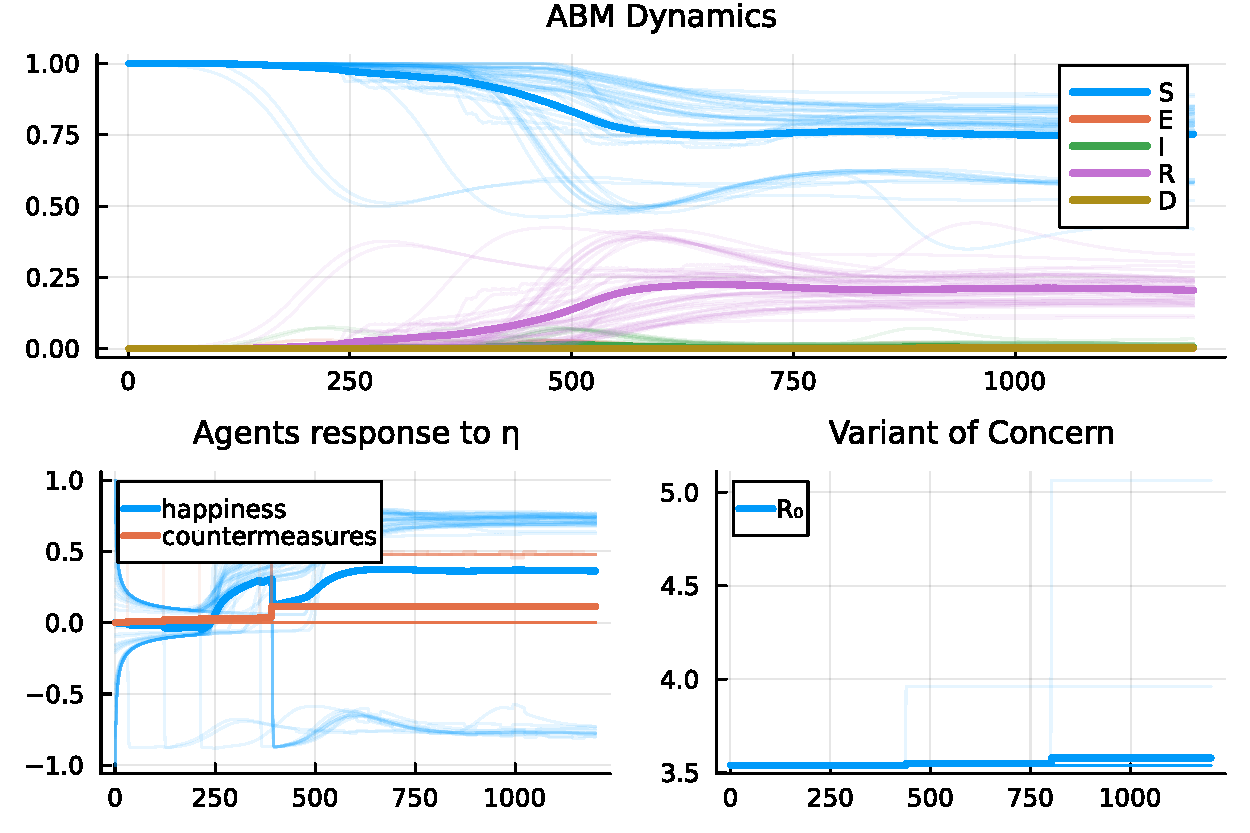
\includegraphics[width=\textwidth]{img/SocialNetworkABM_CONTROL_2023-07-15.pdf}
	\captionof{figure}{Grafico cumulativo del risultato del modello con intervento del controllore}
	\label{fig:abm_intervent}
\end{minipage}

Si puo' notare come le varie curve rappresentate siano molto piu' accentuate mostrando percorsi differenti 
ma comunque simili nell'andamento generale. La curva associata alla felicita' e' altalenante e segue generalmente
l'andamento delle contromisure applicate dal controllore alla popolazione. In questo caso vi sono curve
molto differenti che mostrano comportamenti altrettanto differenti, ma in generale il comportamento e' 
relativamente contenuto e non eccessivo. 

Altro dato interessante e' il numero di VOC che pare essere diminuito rispetto al modello senza intervento.
Questo dipende generalmente dal comportamento delle contromisure. Infatti queste quando vengono applicate, 
oltre a influenzare il parametro \textbf{happiness}, vanno ad influenzare anche la matrice di flusso \ref{fig:migration matrix}
andando a ridurne i valori presenti. Questo fa si che oltre a dilazionare la diffusione della pandemia, andando 
ad applicare involontariamente delle contromisure simil lockdown e smart working (per prevenire il forte afflusso di individui),
va anche a dilazionare il comportamento della funzione che si occupa di generare una VOC \ref{fig:voc}. 

Questa infatti puo' attivarse sse nel nodo sono presenti individui infetti, in quanto non e' stata modellata la 
possibilita' che spontaneamente una nuova variante arrivi in un nuovo nodo senza un veicolo umano. Percio' 
applicare delle contromisure permette anche a contenere la diffusione di VOC nella popolazione osservata.
\subsection{Monitoraggio e Intervento}
Il sistema di controllo e intervento scelto segue l'idea del controllo autonomo tramite l'utilizzo di 
una Neural ODE. Questo approccio permette di specificare un sistema di ODE che descrive il sistema reale 
con le sue relazioni e inserire chirurgicamente una rete neurale al suo interno che controlli il 
dosaggio delle contromisure. \cite{B_ttcher_2022} \cite{innes2019differentiable} \cite{sandoval2022neural}

Questa tecnica permette di ottenere ottimi risultati, i quali tuttavia dipendono fortemente dalla 
tipologia di modellazione del sistema scelto e dalla tipologia di funzione di costo o di controllo 
applicata per addestrare il modello. La sfida in questo caso ricade sull'attenta modellazione del 
sistema di partenza e sulla comprensione dei risultati offerti dal controllore. Questo controllore 
difatti ritorna dei valori nell'ambito $\in[0, 1]$, i quali possono essere difficilmente interpretabili.
Perciò è necessario a priori avere ben chiaro cosa significhi il range di valori che può ritornare
il controllore, e capire a cosa è associato nel mondo reale. 

Inizialmente la funzione di controllo inserita all'interno del modello ad agente è definita 
come riportato in figura \ref{fig:controller_abm}. è possibile osservare come vengano inseriti dei valori di 
controllo per gestire la chiamata al controllore vero e proprio.

I valori di controllo sono generalmente associati a quado bisogna realisticamente parlando, chiamare la 
funzione di controllo. Da un lato servono sia a ridurre il numero di chiamate, e quindi ridurre l'impatto 
prestazionale sia a rendere più realistica l'idea di avere accesso ad un sistema di controllo solamente 
in determinati punti del tempo e non sempre. Questo va ad imitare anche il ritardo tra la raccolta dati, 
la formulazione di una contromisura adeguata e l'applicazione della stessa.

Successivamente vengono definite ulteriori regole di attivazione, questa volta legate alla prima attivazione
del controllore. A posteriori è chiaro come avere delle regole di prevenzione già in atto possa essere di 
enorme aiuto nel combattimento contro il dilagare di un epidemia, ma alle volte vi è un ritardo nel riconoscere
il pericolo, e questo è dato dal valore di \emph{tolerance} il quale non attiva il controllore fintanto che 
la situazione sembra rimanere sotto i minimi di soglia. 

\begin{minipage}{\linewidth}
	\centering
	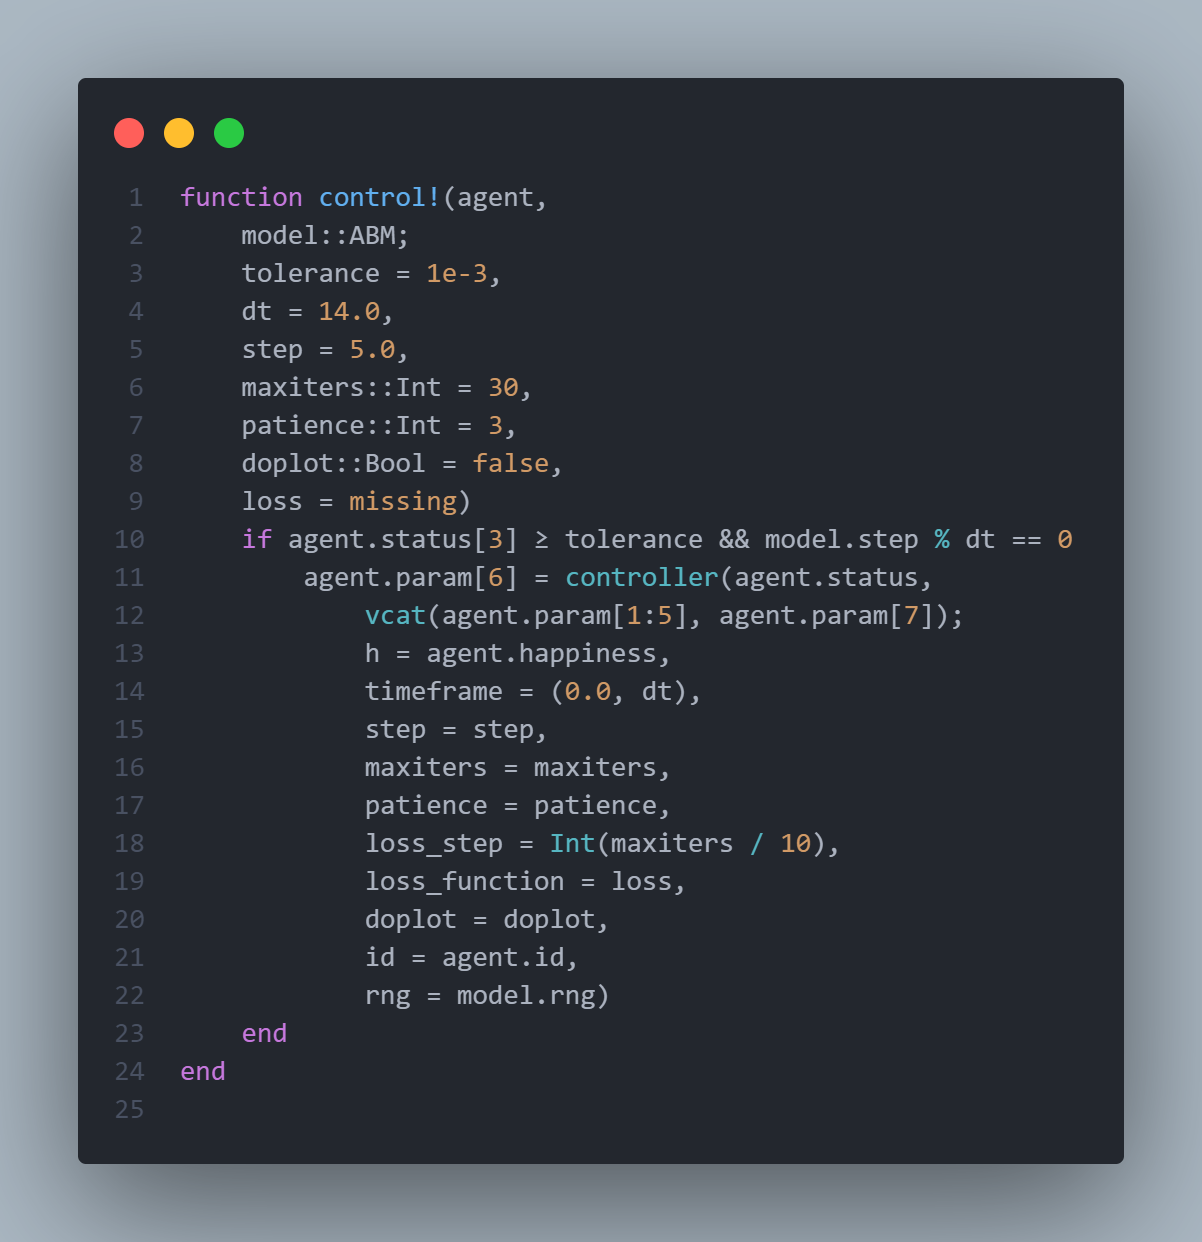
\includegraphics[width=\textwidth]{img/controller_neuralode.png}
	\captionof{figure}{Definizione controller all'interno del modello ad agente}
	\label{fig:controller_abm}
\end{minipage}

Altri valori definiscono principalmente i parametri che servono alla funzione di controllo per operare correttamente.
Tra questi vi è un parametro opzionale $\upsilon$ il quale descrive quanto potrà essere il valore massimo delle 
contromisure applicabili in relazione a quanti infetti sono presenti all'interno di un dato nodo. Questo valore viene 
calcolato come un esponenziale nel numero degli infetti. Questa assunzione è utile come valore di appoggio ulteriore 
per il controllore nel caso in cui dovesse ritornare un valore troppo alto rispetto a quello che di buon senso sarebbe 
adatto. 

\begin{minipage}{\linewidth}
	\centering
	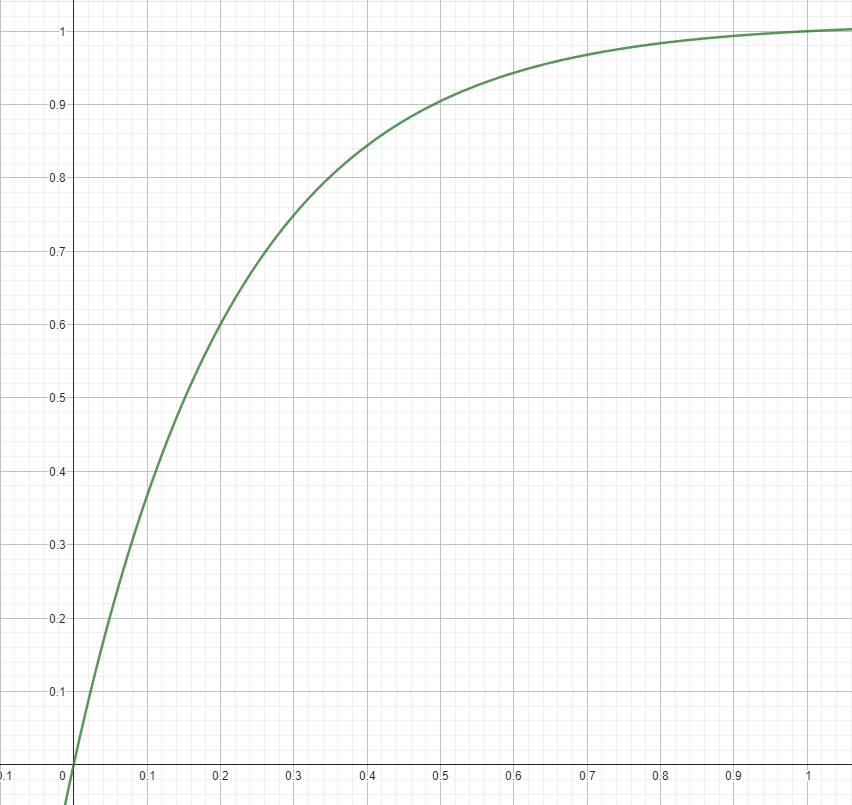
\includegraphics[width=\textwidth]{img/activationfunction_controller.png}
	\captionof{figure}{Funzione per il calcolo del limite superiore per le contromisure}
	\label{fig:max_countermeasures_function_abm}
\end{minipage}

Come si può osservare, la funzione descritta in figura \ref{fig:max_countermeasures_function_abm} 
è ottenibile dalla seguente formula: $\frac{e^{k \cdot x}-1}{e^{k}-1}$, in particolare la funzione sopra 
presentata è ottenuta dal valore $k = -4.5$. Questo tipo di funzione è stata scelta in quanto descrive abbastanza 
bene il valore di pericolo che, soprattutto durante i primi mesi di pandemia, è stato attribuito al numero di infetti che 
si riscontravano. Questo valore cresce rapidamente e poi tende a rallentare abbastanza bruscamente una volta superata la 
soglia del cinquanta percento di infetti. 

Questo può essere anche relazionato all'idea che una pandemia abbia un punto critico dopo il quale le speranze decadono. Questo 
ovviamente in relazione alla pandemia stessa. Questa funzione potrebbe anche alterarsi nel corso del tempo, modellando perciò 
una sorta di abitudine alla pandemia. 

Il controllore vero e proprio si articola principalmente come già accennatto nella sezione relativa alle Neural ODE. 

\begin{minipage}{\linewidth}
	\centering
	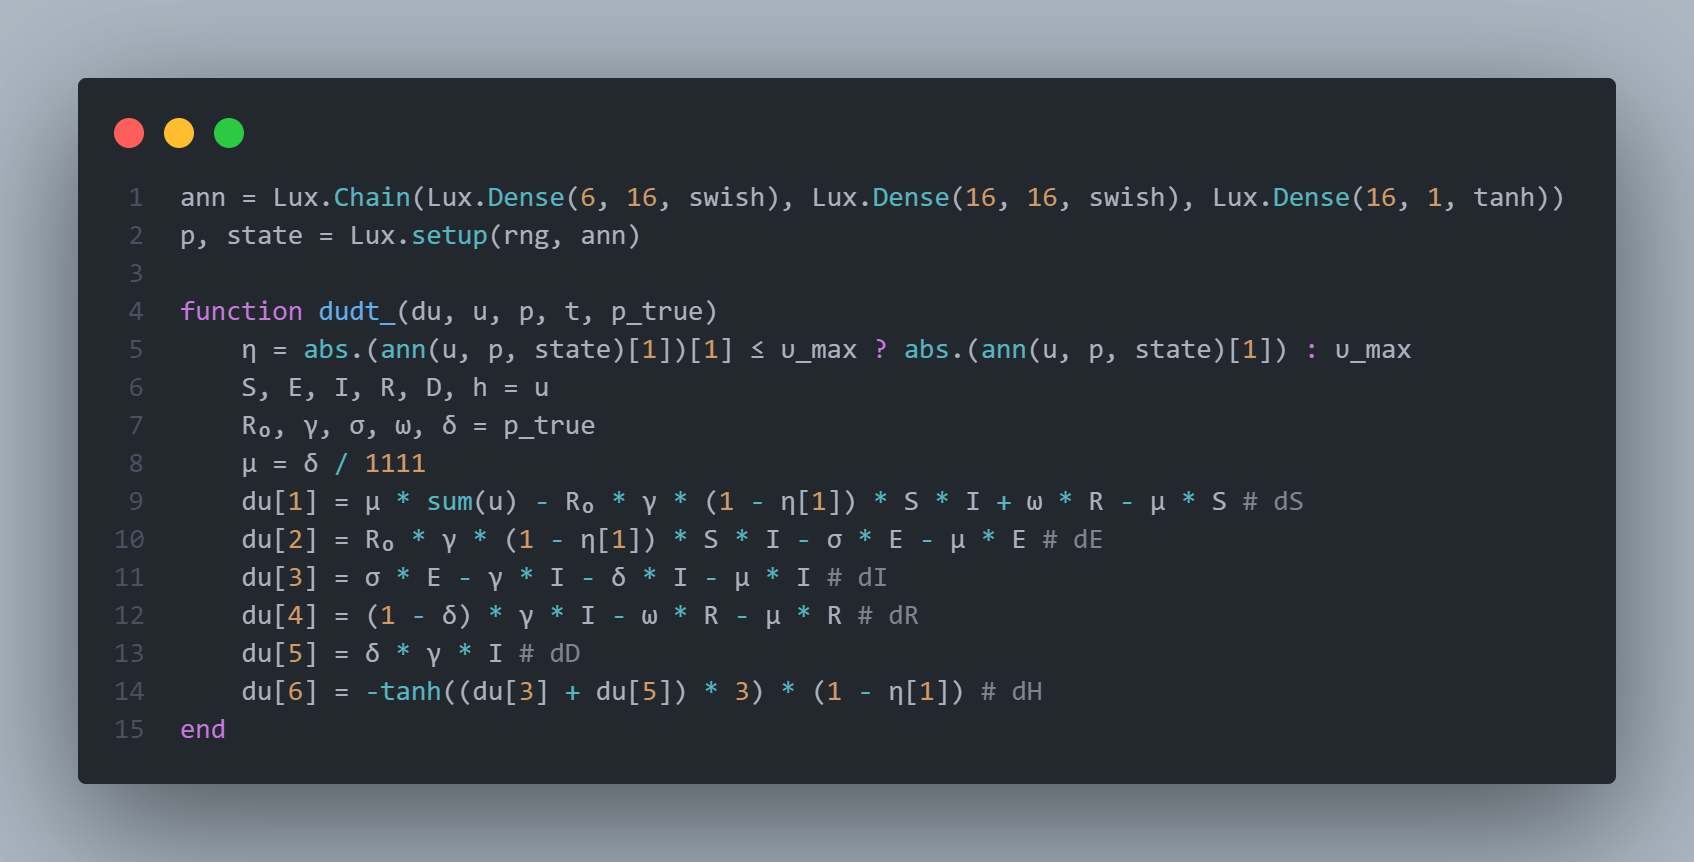
\includegraphics[width=\textwidth]{img/controller1.png}
	\captionof{figure}{Definizione controllore tramite Neural ODE}
	\label{fig:controller1}
\end{minipage}

Viene definita una rete neurale tramite l'ausilio del framework \textbf{Lux.jl} \cite{pal2023lux}, e questa viene utilizzata
esclusivamente per il guess del valore di controllo $\eta$ durante la fase di addestramento, il quale verrà 
alla fine utilizzato come valore di controllo per il modello. Successivamente viene definito il sistema di ODE che governa il fenomeno che vogliamo analizzare, nello specifico il sistema in 
questione è un sistema \textbf{SEIR} che modella la perdita di immunità con il tempo. 

Successivamente viene istanziato il problema con l'ausilio dell'interfaccia \textbf{ODEProblem} e da qui in avanti il modello potrà iniziare a 
essere allenato. Innanzitutto vengono definite delle funzioni per la predizione e il calcolo della loss del modello, 
e infine anche una funzione ausiliaria di callback utile per osservare l'andamento dell'apprendimento del modello.

\begin{minipage}{\linewidth}
	\centering
	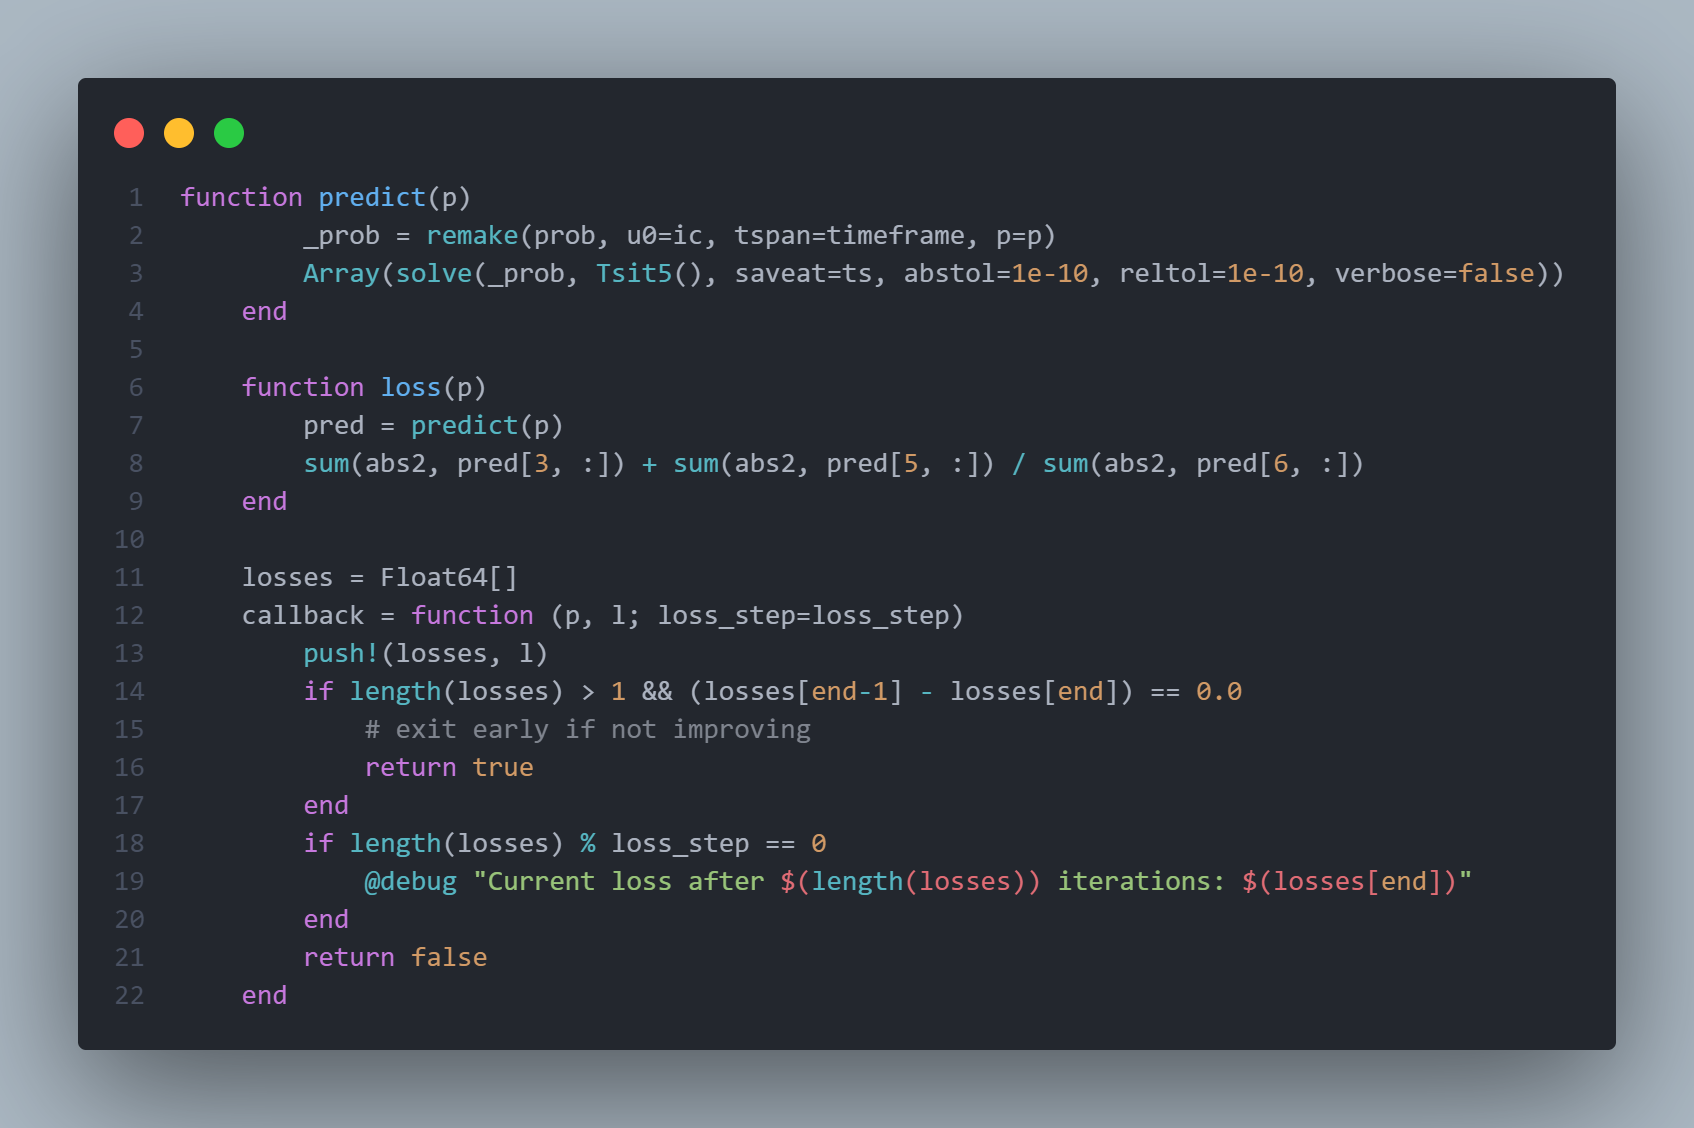
\includegraphics[width=\textwidth]{img/controller2.png}
	\captionof{figure}{Definizione funzioni di appoggio del controllore}
	\label{fig:controller2}
\end{minipage}

Come si può osservare in figura \ref{fig:controller2} la funzione di \emph{callback} oltre ad essere una funzione di 
appoggio nella stampa dei dati relativi all'addestramento, è anche una utile funzione per implementare un controllo sulla tipologia 
di apprendimento del modello. Infatti per ridurre ancora di più il numero di iterazioni necessarie per avere dei buoni risultati 
è stato scelto di inserire un controllo simile al metodo di \textbf{early stopping} \cite{wiki:Early_stopping} per prevenire 
l'addestramento eccessivo quando si trova un valore di ottimo. Questo approccio è puramente \emph{empirico} in quanto 
è stato riscontrato come il valore di loss generale del sistema tende a decrescere o crescere stabilmente e una volta trovato il 
valore ottimale, se rimangono delle iterazioni da fare, questo non migliora per cui una volta che i valori rimangono identici 
è un buon azzardo terminare il periodo di addestramento del modello.

La parte di addestramento vero e proprio del modello avviene con le seguenti funzioni

\begin{minipage}{\linewidth}
	\centering
	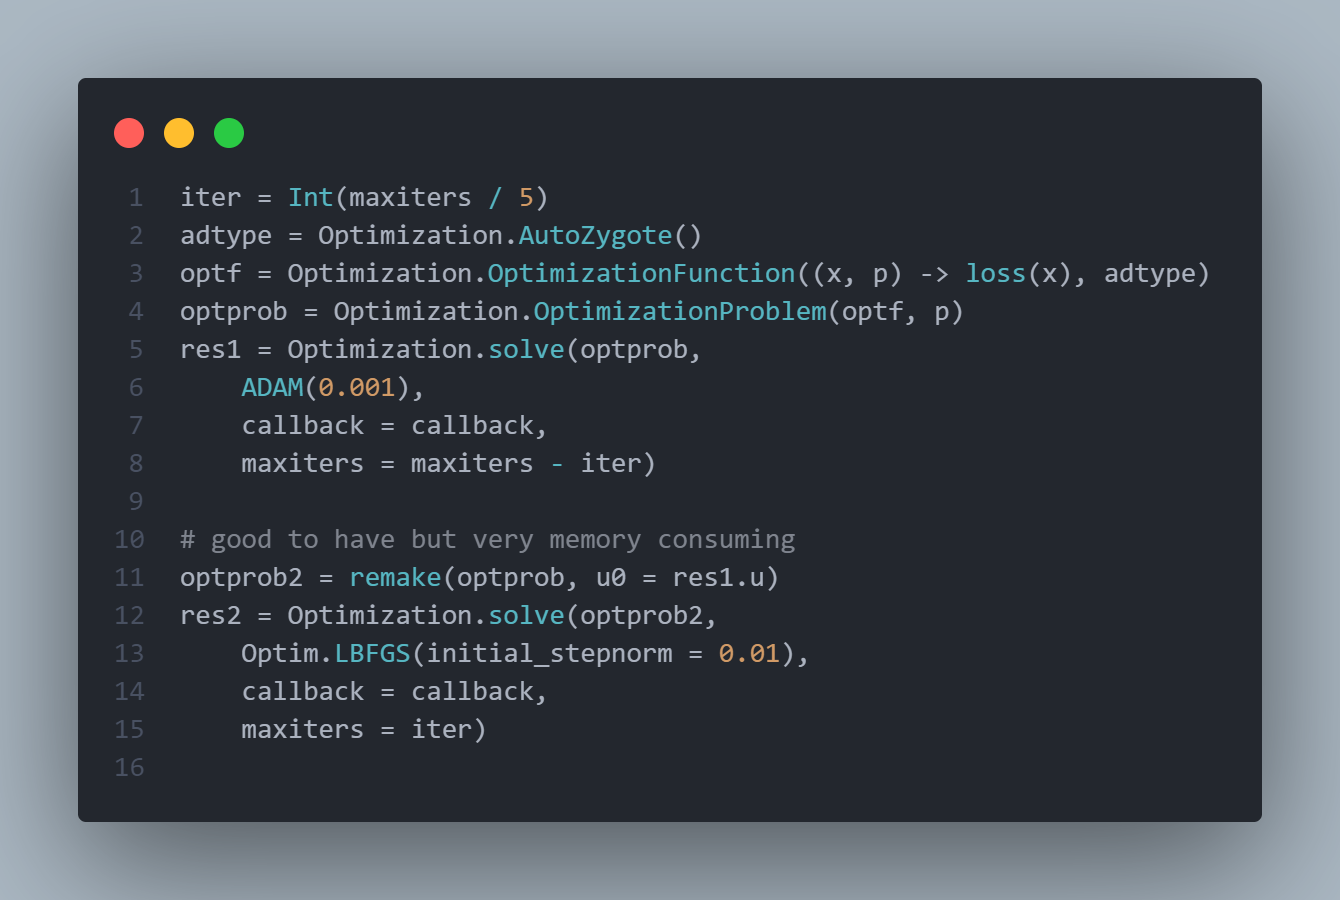
\includegraphics[width=\textwidth]{img/controller3.png}
	\captionof{figure}{Definizione funzioni di addestramento del controllore}
	\label{fig:controller3}
\end{minipage}

Il ciclo di addestramento può essere scomposto idealmente in due parti, ma per quanto osservato, non sono 
entrambe necessarie. La prima parte, riportata in figura \ref{fig:controller3} si propone di utilizzare un ciclo di addestramento 
con l'utilizzo dell'ottimizzatore \textbf{ADAM}. Se i risultati dovessero esser soddisfacenti, allora è possibile terminare. 
Tuttavia in questi casi, è buona pratica utilizzare due differenti cicli di addestramento per migliorare i risultati. 

Più nello specifico vengono associati due differenti cicli di addestramento con due differenti ottimizzatori per ottenere il massimo 
da entrambi. Questo approccio serve per massimizzare le peculiarità di ognuno degli ottimizzatori. è pratica comune utilizzare per la 
buona parte dell'addestramento un ottimizzatore in grado di trovare un buono spazio degli iperparametri e successivamente utilizzare 
un ottimizzatore come ad esempio \textbf{BFGS} \cite{10.1093/imamat/6.1.76} \cite{35d0019d-775a-3628-b0b4-67be112e346b} \cite{10.1093/comjnl/13.3.317} \cite{e3177091-3094-3792-9d61-0ab445735ddb}
il quale è estremamente utile nel trovare rapidamente un minimo locale all'interno dello spazio dei parametri.

L'utilizzo di questi due ottimizzatori in successione è utile in quanto utilizzando solamente \textbf{ADAM} si potrebbe 
incorrere nell'avere un numero di iterazioni troppo elevate per raggiungere lo stesso risultato, mentre utilizzando solamente \textbf{BFGS} si 
potrebbe incorrere in un brutto minimo locale.

La mia scelta di non utilizzare l'approccio sopra descritto, ovvero di utilizzare due differenti ottimizzatori per 
ottenere il massimo risultato da entrambi, è dato dal fatto che generalmente l'utilizzo di ADAM 
con un numero di iterazioni molto contenuto, dato anche dall'utilizzo di una tecnica per ridurre ulteriormente
le iterazioni di addestramento se non vi è un guadagno di accuratezza \ref{fig:controller2}, 
permette di arrivare al miglior risultato in breve tempo senza l'utilizzo di un 
secondo ottimizzatore, il quale se comunque utilizzato non porta alcun 
miglioramento di sorta, impegnando solamente risorse computazionali.

\begin{minipage}{\linewidth}
	\centering
	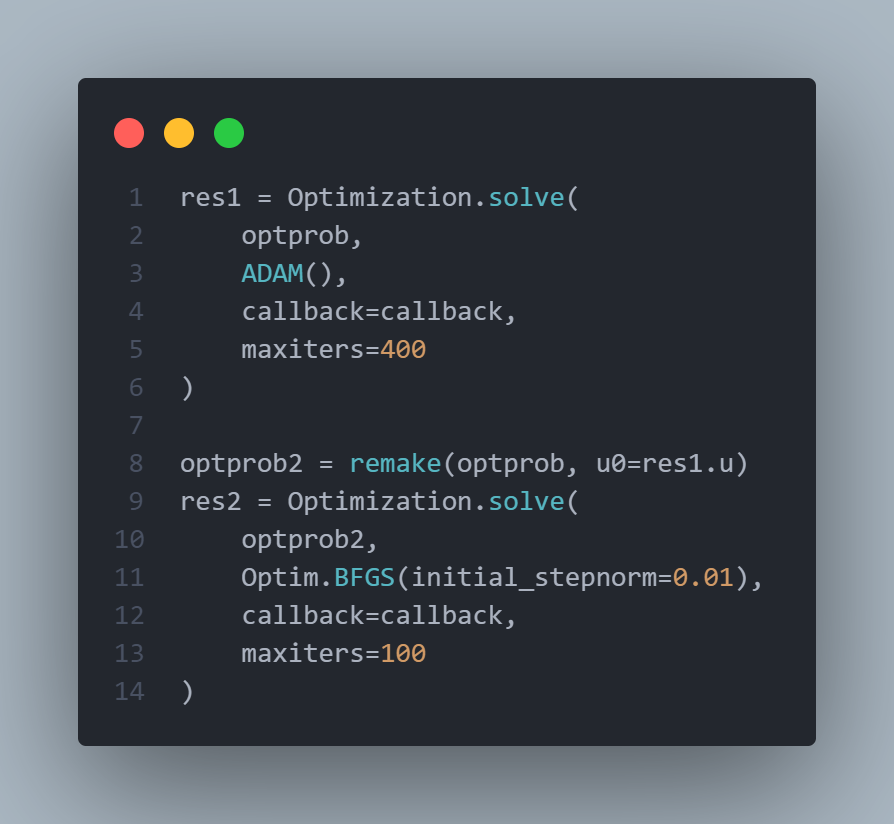
\includegraphics[width=\textwidth]{img/optimizers_example.png}
	\captionof{figure}{Esempio di utilizzo congiunto di due ottimizzatori differenti in uno stesso ciclo di addestramento}
	\label{fig:two_otpimizers}
\end{minipage}

\subsubsection*{Funzione di attivazione rete neurale}
% inserisci qualcosa in più
La scelta della funzione di attivazione all'interno delle reti neurali pone un grande impatto sulle 
dinamiche di apprendimento. Attualmente la più utilizzata e di grande successo è la \textbf{ReLU}
(\textbf{Re}ctified \textbf{L}inear \textbf{U}nit) la quale è della forma $f(x) = max(0,x)$. 
Tuttavia svariate alternative sono state proposte, ma nessuna di queste è riuscita a 
spodestare il primato della ReLU, principalmente a causa di guadagni prestazionali inconsistenti. 

La funzione di attivazione che ho deciso di utilizzare si chiama \textbf{Swish} ed è stata proposta dal 
\emph{Google Brain Team} \cite{ramachandran2017searching}, la quale è la seguente funzione $f(x) = x \cdot sigmoid(x)$. 
Nei loro esperimenti è stato osservato come sostituire la funzione di attivazione ReLU con Swish permetteva 
di avere un aumento prestazionale sui task di \emph{top-1 classification} sul dataset \textbf{ImageNet} del $0.9\%$ utilizzando
\textbf{NASNetA} e dello $0.6\%$ utilizzado \textbf{Inception-ResNet-v2}. 

\begin{minipage}{\linewidth}
	\centering
	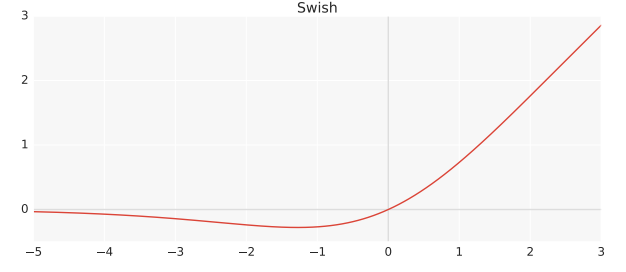
\includegraphics[width=\textwidth]{img/Screen-Shot-2017-10-18-at-2.39.55-PM.png}
	\captionof{figure}{Funzione di attivazione Swish}
	\label{fig:swish}
\end{minipage}

Il punto forte di Swish è la sua semplicità e forte somiglianza con ReLU, la quale la rende estremamente facile da implementare
al suo posto. La principale problematica con l'utilizzo di ReLU è il fatto che il valore della derivata è 0 per metà 
dei valori in input $x$. 

è stato dimostrato come, utilizzando il dataset \textbf{MNIST}, le prestazioni di Swish e ReLU siano 
equiparabili nei fintanto che le reti avevano un numero di layer all'incirca fino a 40. Successivamente Swish riusciva ad ottenere 
prestazioni migliori di ReLU in maniera considerevole, soprattutto quando il numero di layer si attestava tra i 40 e i 50, casi 
in cui l'ottimizzazione tendenzialmente diventa più complessa. Questo suggeri, e venne poi osservato, come 
in reti molto profonde, Swish tendeva ad avere prestazioni migliori nei test di accuracy rispetto alla controparte presa in esame. 
Entrambe comunque hanno esperienziato un calo delle prestazioni all'aumentare della dimensioni dei batch; in ogni caso comunque Swish otteneva 
dei risultati migliori. 

Alla luce di questi dati ho deciso di utilizzare questa funzione come funzione di attivazione all'interno della rete neurale, 
anche se tendenzialmente essendo essa poco profonda, i risultati e soprattutto il guadagno di accuratezza non dovrebbe essere troppo sensibile \ref{fig:controller1}.

% discussione dei risultati ottenuti
\section{Analisi di Sensibilità}

L'analisi di sensitività è stata condotta sul modello SEIR, 
come illustrato in Figura \ref{fig:ODE_Julia_example}. 
Questa analisi mirava a valutare come il modello reagisse a 
variazioni specifiche dei suoi parametri, le quali potrebbero 
condurre a comportamenti inattesi o peculiari.

Per effettuare l'analisi di sensitività, sono stati impiegati i 
metodi forniti dalla suite SciML.ai. Ciò ha permesso di identificare 
i parametri ai quali il modello è più sensibile.

\begin{figure}[H]
    \begin{center}
		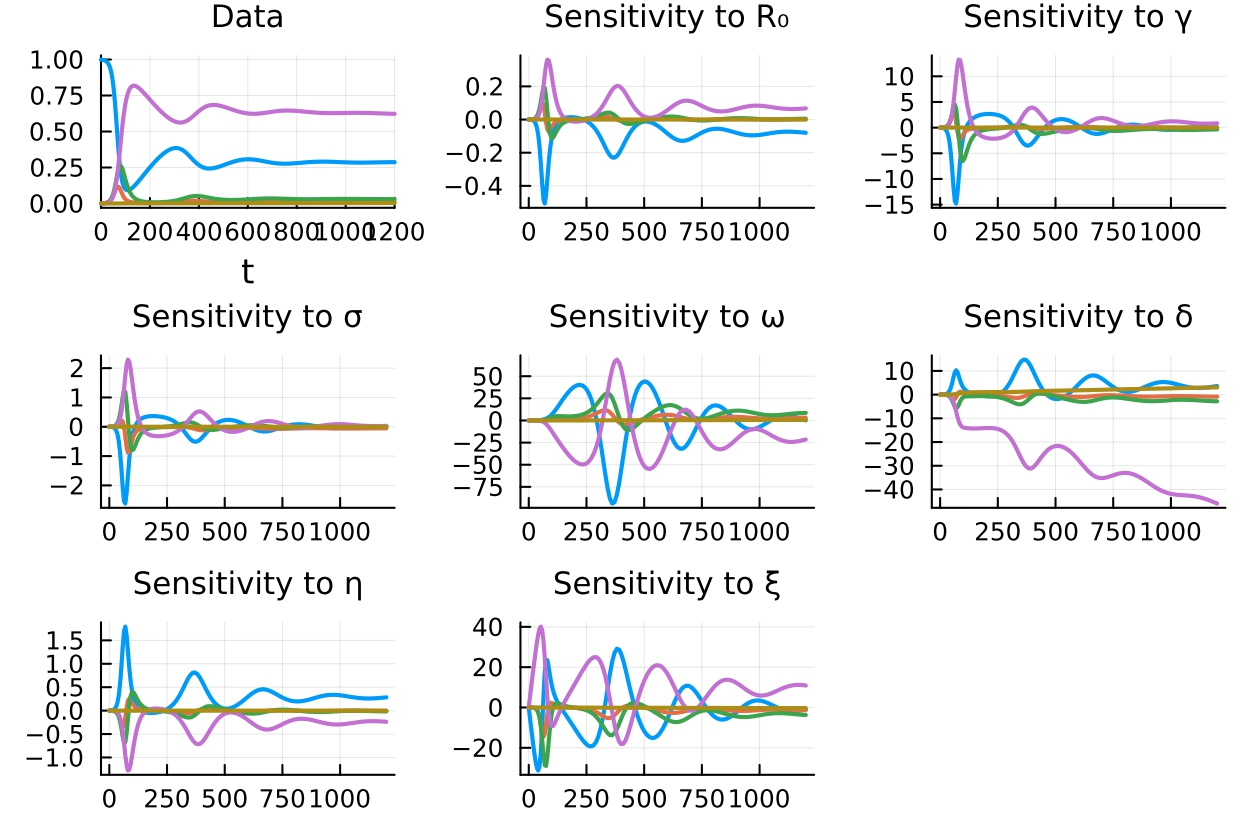
\includegraphics[width=\textwidth]{img/sa.jpg}
		\caption{Grafico rappresentante l'analisi di sensitività del modello}
		\label{fig:sens_anal}
	\end{center}
\end{figure}

Come evidenziato nella Figura \ref{fig:sens_anal}, il modello 
dimostra una sensitività uniforme rispetto ai parametri 
$R_0$, $\gamma$, e $\sigma$, il che è coerente, dato che essi 
influiscono sull'andamento dell'epidemia. La sensitività ai parametri 
$\omega$ e $\delta$ era attesa, ma è risultata più marcata di 
quanto previsto. La sensitività al parametro $\eta$, che influisce 
sulle contromisure, è inversamente correlata a quella del 
parametro $R_0$, come previsto, poiché $\eta$ è direttamente 
legato alle misure di contenimento. La sensitività al parametro 
$\xi$ mostra un comportamento singolare, probabilmente dovuto 
alla sua correlazione con $\omega$, entrambi legati al compartimento 
``R'' del modello, che gestisce gli individui guariti e vaccinati.

In una fase successiva dell'analisi, è stata condotta un'analisi di 
sensitività sui parametri specifici del modello ad agenti, 
utilizzando la funzione \textbf{paramscan} fornita dalla libreria 
\textbf{Agents.jl}. Sono stati individuati e selezionati quei 
parametri che potrebbero avere un notevole impatto sul comportamento 
generale del modello. Questa selezione è stata fatta in base al 
potenziale di tali parametri di innescare cambiamenti significativi nei 
risultati della simulazione.

È importante notare che alcuni parametri, specificamente quelli 
legati al controllore e alla campagna di vaccinazione, sono stati 
esclusi da questa analisi. Ciò è dovuto al fatto che variazioni in 
questi parametri possono comportare cambiamenti sostanziali nella 
simulazione, e pertanto sono stati considerati separatamente e 
successivamente analizzati in modo dettagliato.

\begin{figure}[H]
    \begin{center}
		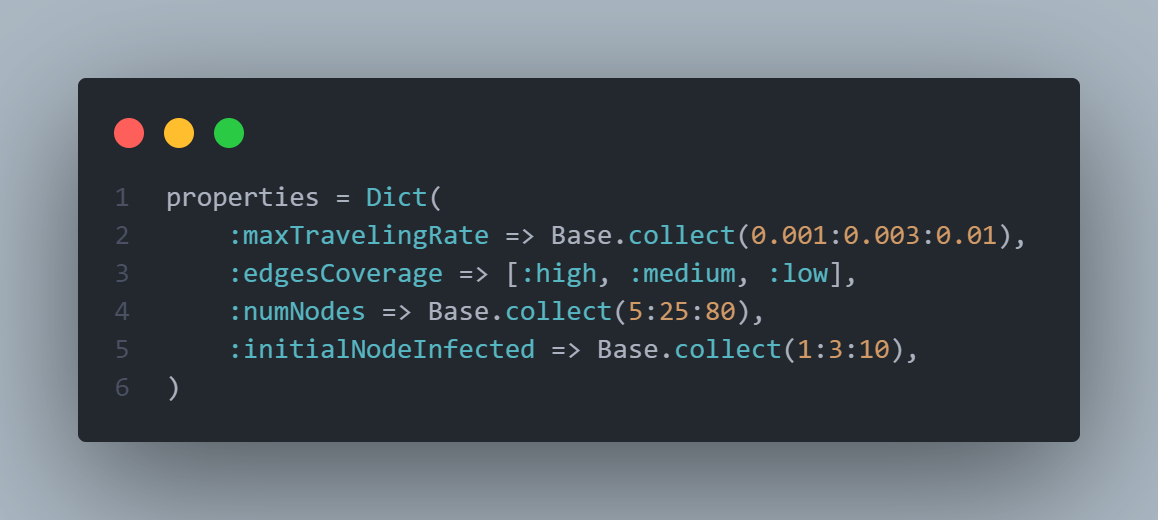
\includegraphics[width=\textwidth]{img/paramscan.png}
		\caption{Parametri usati per l'analisi di sensitività del modello ad agente}
		\label{fig:paramscan}
	\end{center}
\end{figure}

L'analisi di sensitività sui parametri rimanenti mira a esplorare 
come variazioni specifiche in ciascuno di essi possano influenzare 
il comportamento complessivo del modello. Questo tipo di analisi è 
fondamentale per comprendere la sensibilità del sistema a variazioni 
nei parametri e per valutare le risposte del modello a differenti 
condizioni.

In definitiva, questa analisi di sensitività fornisce un quadro più 
completo della dinamica del modello, consentendo di identificare i 
parametri chiave che influenzano le sue prestazioni e fornendo 
indicazioni importanti per la calibrazione e l'ottimizzazione del 
modello stesso.
\newpage

\subsection{Analisi del Comportamento in Base al Numero Iniziale di Nodi Infetti}

L'analisi condotta ha investigato l'impatto del numero iniziale di 
nodi infetti sul comportamento complessivo del modello. 
I risultati hanno dimostrato che un numero maggiore di nodi infetti 
iniziali conduce a un raggiungimento più rapido del picco di infetti 
nel corso della simulazione. Tuttavia, non sono stati osservati altri 
cambiamenti significativi nel comportamento del modello.

Questo risultato era atteso e coerenza con le dinamiche epidemiologiche 
conosciute. Infatti, è noto che un aumento del numero iniziale di 
individui infetti in una popolazione può accelerare l'espansione della 
malattia e portare a un picco di infetti più precoce. 
Tuttavia, le altre dinamiche del modello, come il tasso di diffusione 
del virus, la progressione della pandemia e le misure di intervento, 
non sono state influenzate in modo significativo da questa variazione.

\begin{figure}[H]
	\centering
	\begin{subfigure}[b]{0.45\textwidth}
		\centering
		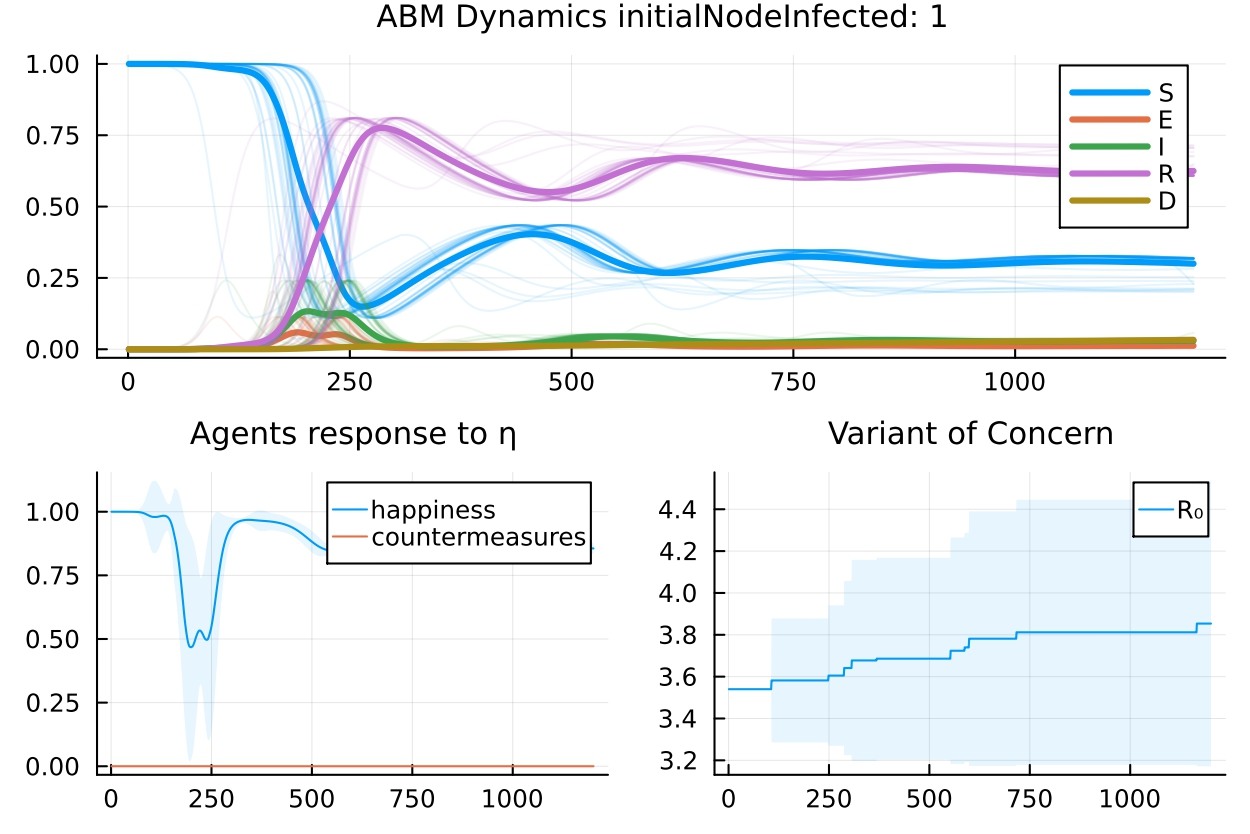
\includegraphics[width=\textwidth]{img/SocialNetworkABM_1_II.jpg}
		\caption{Grafico per la comparazione sul numero di nodi infetti di partenza. Numero nodi infetti iniziali 1}
		\label{fig:comparison_init_node_inf_1}
	\end{subfigure}
	\hfill
	\begin{subfigure}[b]{0.45\textwidth}
		\centering
		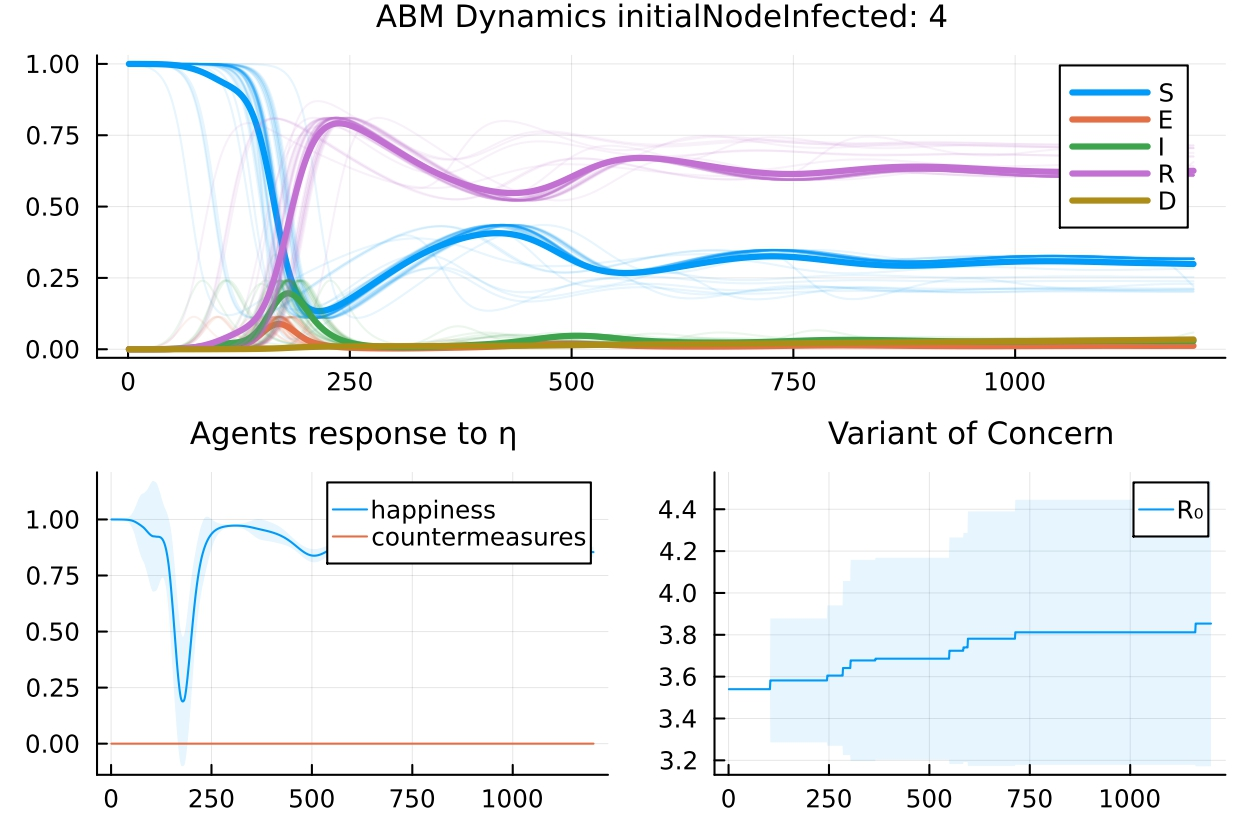
\includegraphics[width=\textwidth]{img/SocialNetworkABM_2_II.jpg}
		\caption{Grafico per la comparazione sul numero di nodi infetti di partenza. Numero nodi infetti iniziali 4}
		\label{fig:comparison_init_node_inf_4}
	\end{subfigure}
	\hfill
	\begin{subfigure}[b]{0.45\textwidth}
		\centering
		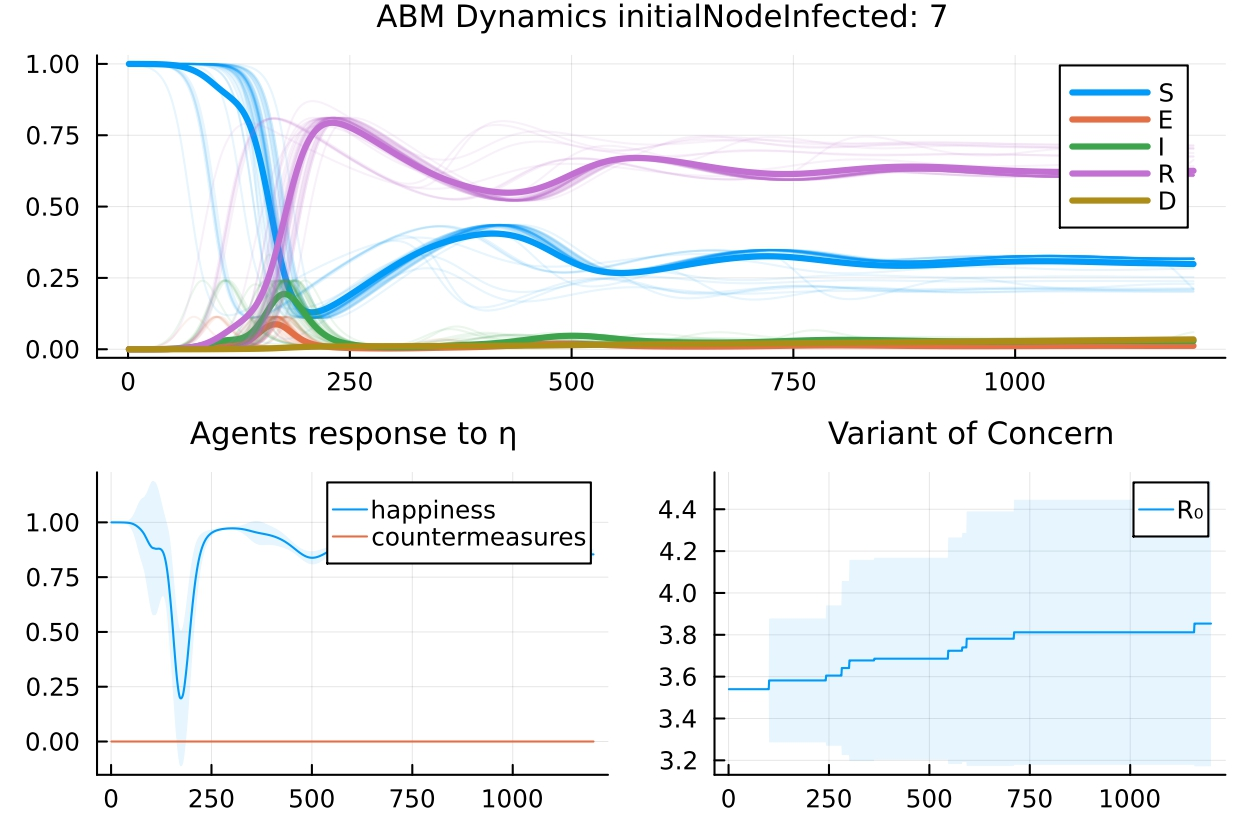
\includegraphics[width=\textwidth]{img/SocialNetworkABM_3_II.jpg}
		\caption{Grafico per la comparazione sul numero di nodi infetti di partenza. Numero nodi infetti iniziali 7}
		\label{fig:comparison_init_node_inf_7}
	\end{subfigure}
	\hfill
	\begin{subfigure}[b]{0.45\textwidth}
		\centering
		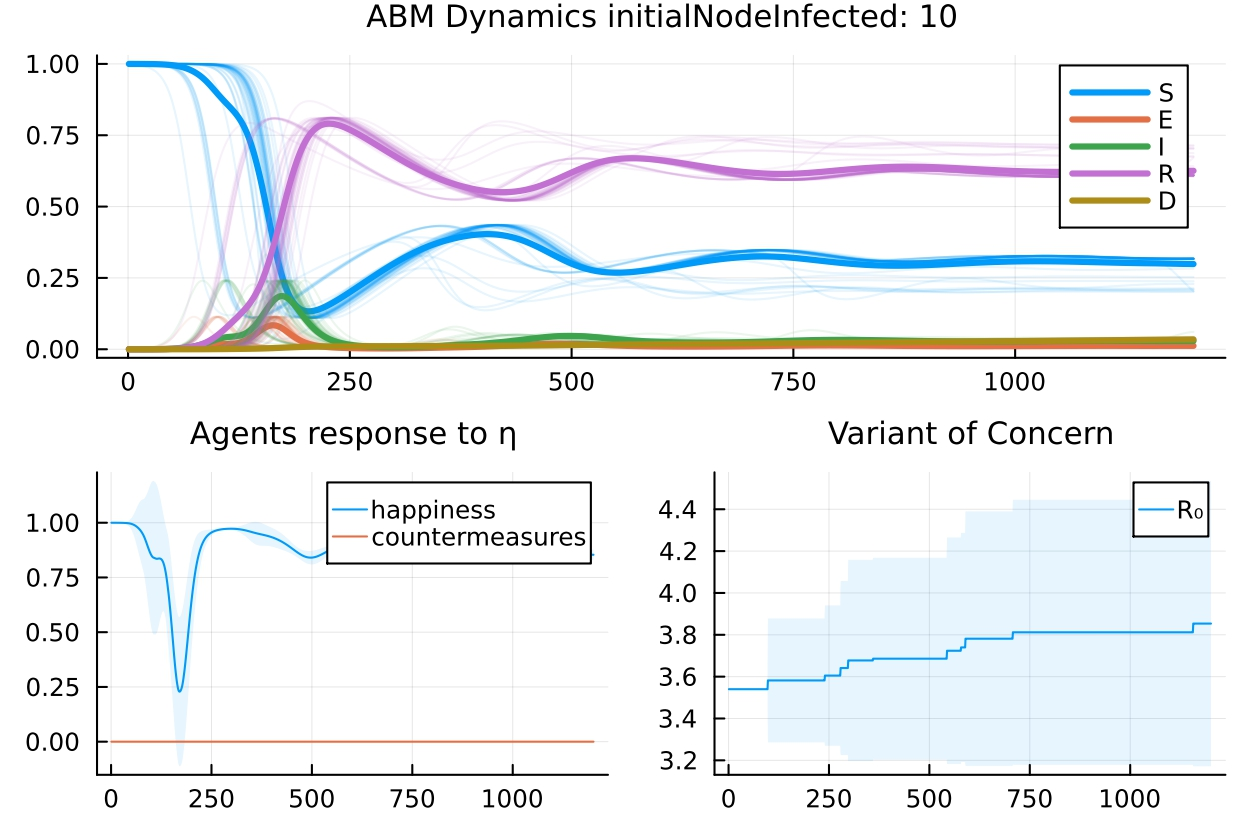
\includegraphics[width=\textwidth]{img/SocialNetworkABM_4_II.jpg}
		\caption{Grafico per la comparazione sul numero di nodi infetti di partenza. Numero nodi infetti iniziali 10}
		\label{fig:comparison_init_node_inf_10}
	\end{subfigure}
\end{figure}

In definitiva, questo risultato conferma la validità delle dinamiche 
epidemiologiche incorporate nel modello e suggerisce che il modello sia 
in grado di riflettere realisticamente l'effetto del numero iniziale di 
infetti sulla diffusione della pandemia, come si verifica anche nella 
realtà.

\subsection{Analisi del Comportamento in Base al Tasso di Migrazione}

L'analisi condotta ha esplorato l'influenza del tasso di migrazione sul 
comportamento del modello. I risultati hanno evidenziato che un tasso di 
migrazione più elevato ha generato un picco di individui infetti più alto, 
e ciò è avvenuto in un periodo di tempo più breve rispetto ai casi in cui 
il tasso di migrazione era più basso.

Questo risultato è coerente con le conoscenze consolidate riguardo 
all'effetto della mobilità sulla diffusione delle malattie infettive. 
Infatti, un aumento del tasso di migrazione implica un maggiore movimento 
delle persone tra i nodi del grafo (rappresentanti aree geografiche o 
comunità), il che può facilitare la trasmissione del virus da un luogo 
all'altro. Di conseguenza, si verifica un aumento più rapido e 
pronunciato nel numero di individui infetti, portando a un picco più 
alto in un tempo più breve.

\begin{figure}[H]
	\centering
	\begin{subfigure}[b]{0.45\textwidth}
		\centering
		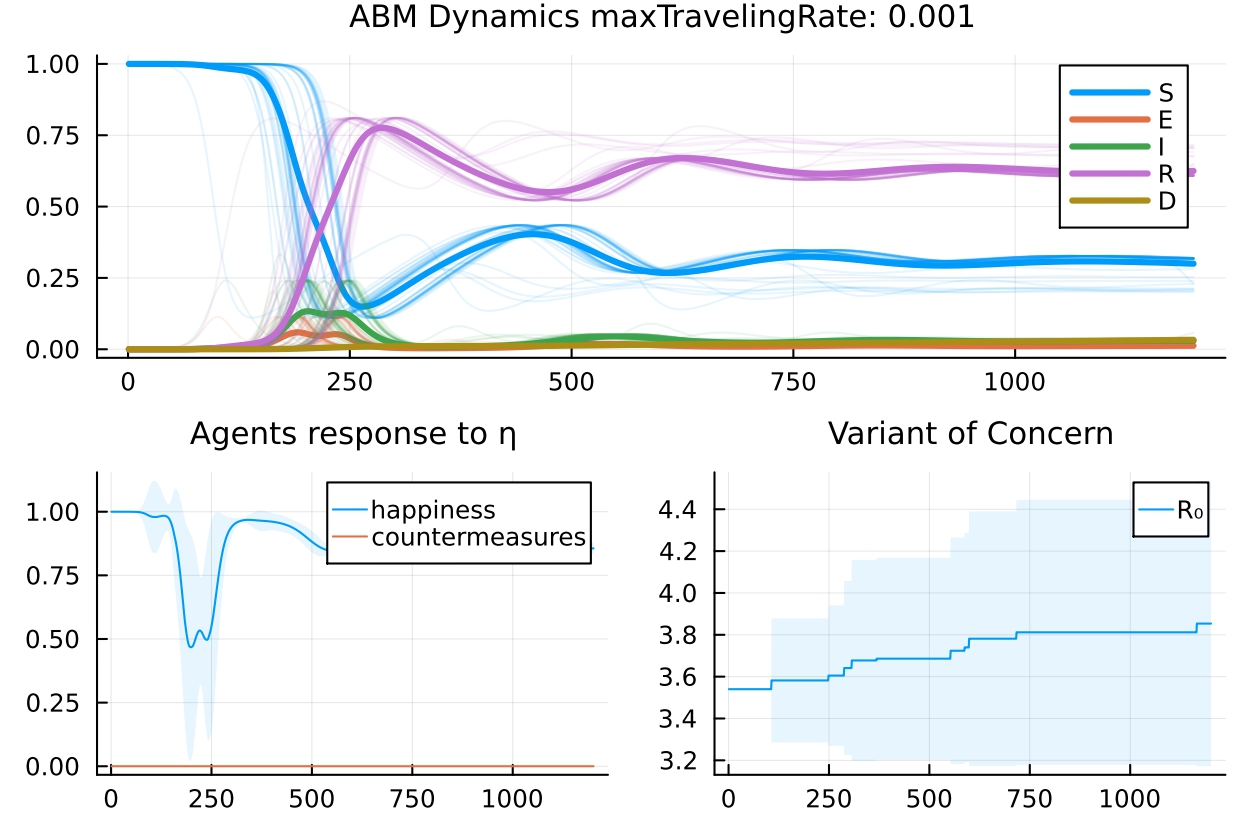
\includegraphics[width=\textwidth]{img/SocialNetworkABM_1_MTR.jpg}
		\caption{Grafico per la comparazione sul valore di migrazione. Valore di 0.001}
		\label{fig:comparison_maxTravelingRate_low}
	\end{subfigure}
	\hfill
	\begin{subfigure}[b]{0.45\textwidth}
		\centering
		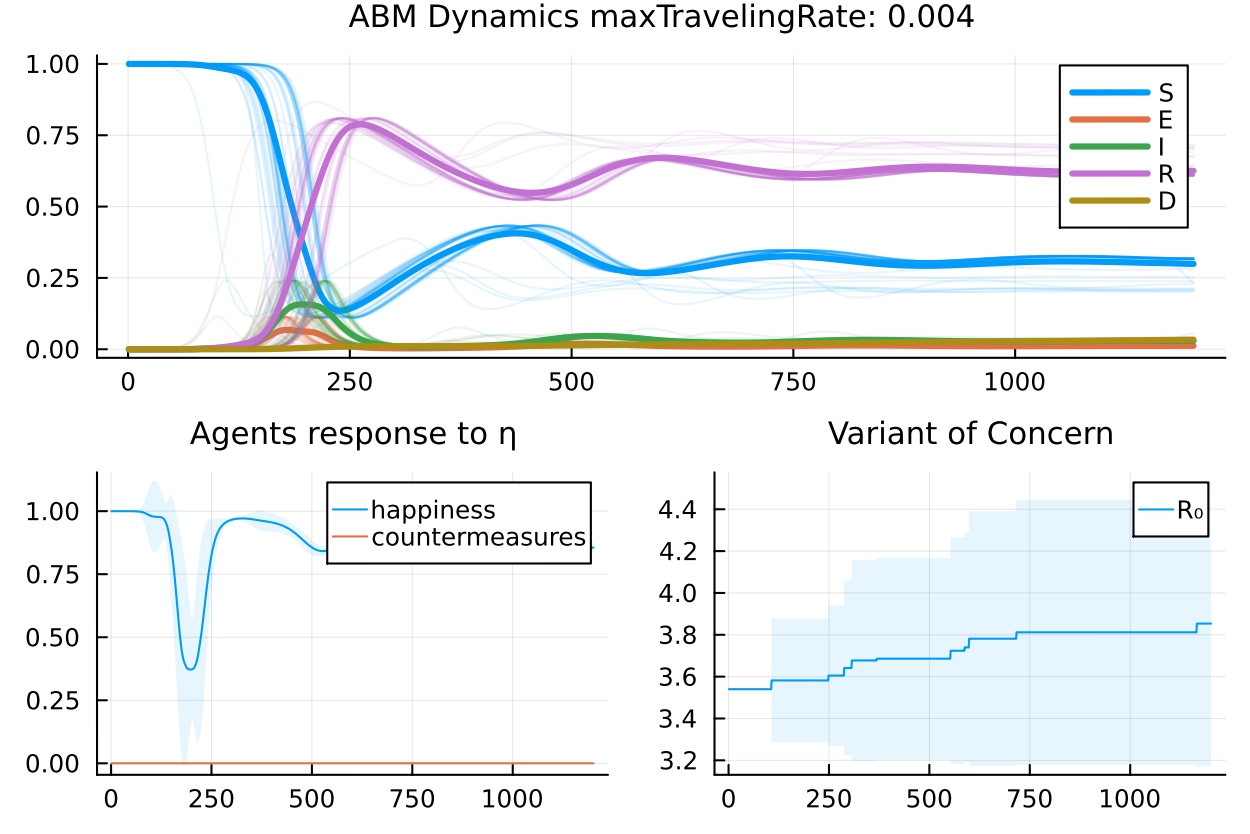
\includegraphics[width=\textwidth]{img/SocialNetworkABM_2_MTR.jpg}
		\caption{Grafico per la comparazione sul valore di migrazione. Valore di 0.004}
		\label{fig:comparison_maxTravelingRate_midl}
	\end{subfigure}
	\hfill
	\begin{subfigure}[b]{0.45\textwidth}
		\centering
		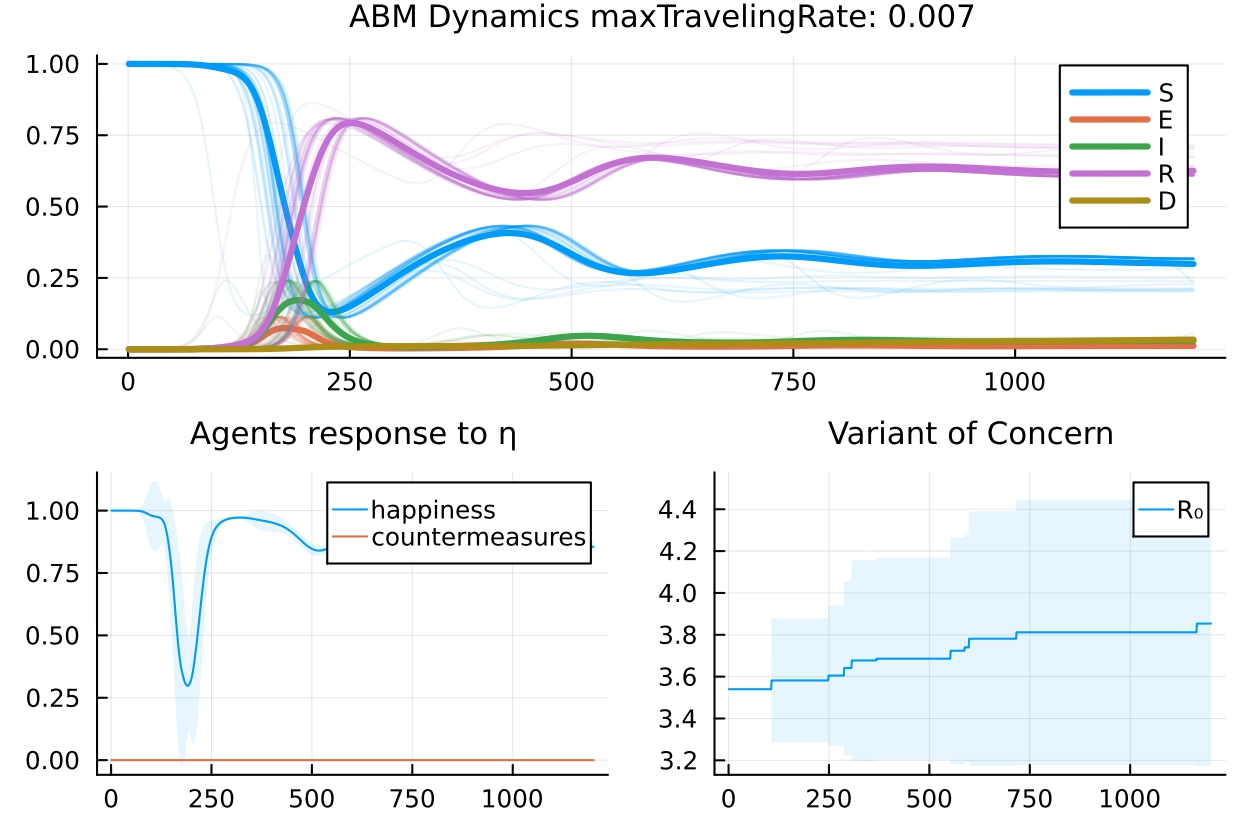
\includegraphics[width=\textwidth]{img/SocialNetworkABM_3_MTR.jpg}
		\caption{Grafico per la comparazione sul valore di migrazione. Valore di 0.007}
		\label{fig:comparison_maxTravelingRate_midh}
	\end{subfigure}
	\hfill
	\begin{subfigure}[b]{0.45\textwidth}
		\centering
		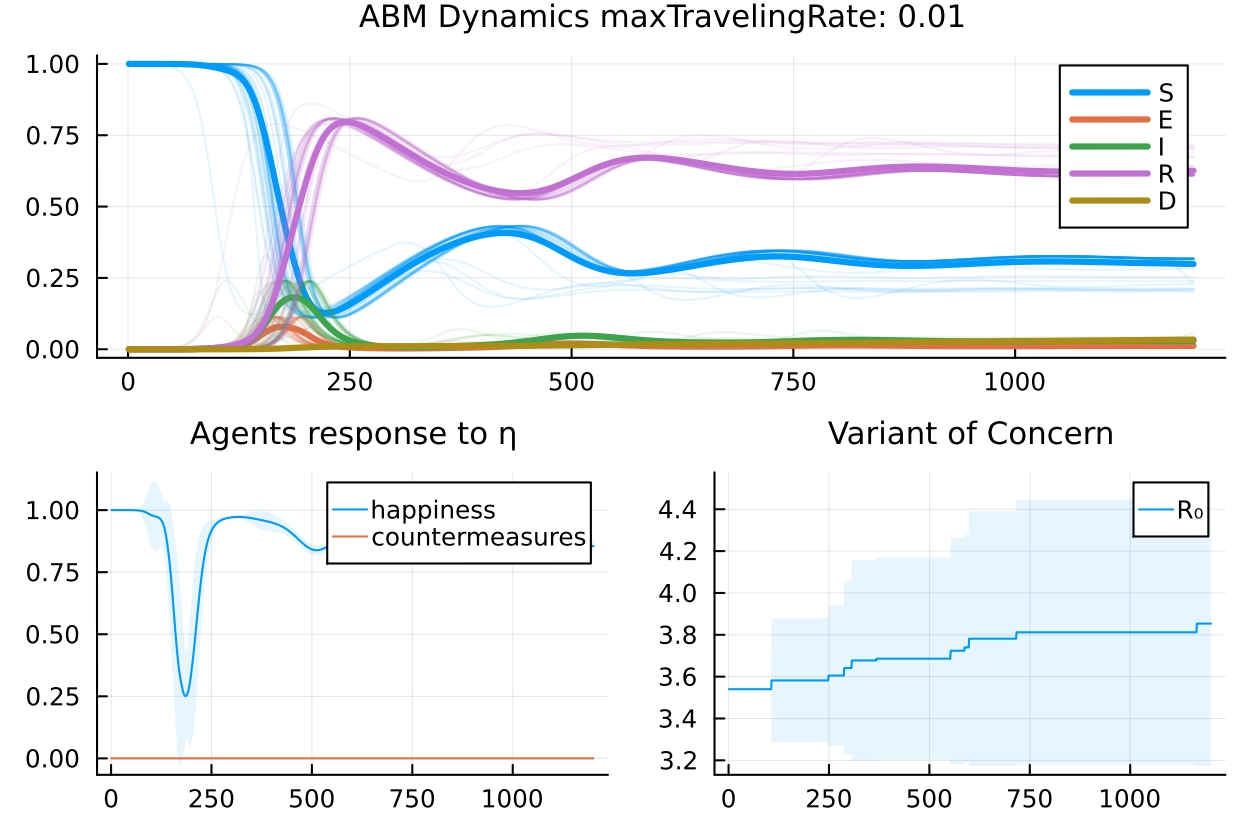
\includegraphics[width=\textwidth]{img/SocialNetworkABM_4_MTR.jpg}
		\caption{Grafico per la comparazione sul valore di migrazione. Valore di 0.01}
		\label{fig:comparison_maxTravelingRate_high}
	\end{subfigure}
\end{figure}

Questi risultati sottolineano l'importanza della mobilità e dei flussi 
di persone nel contesto della diffusione di malattie infettive, come le 
pandemie. Essi sottolineano anche la capacità del modello di catturare 
in modo realistico queste dinamiche epidemiologiche, consentendo una 
valutazione approfondita degli effetti del tasso di migrazione sul 
comportamento del sistema.

\subsection{Analisi del Comportamento in Base al Numero di Nodi della Rete}

L'analisi condotta ha investigato come il numero di nodi nella rete 
influenzi il comportamento complessivo del modello. 
Dai risultati è emerso che un numero maggiore di nodi nella rete ha 
comportato una diffusione più lenta della pandemia e ha generato picchi 
meno ripidi ma più prolungati nel tempo.

Questo risultato è influenzato da diversi fattori, tra cui la 
topologia delle connessioni tra i nodi e la posizione del focolaio 
iniziale della pandemia. Quando ci sono più nodi nella rete, 
la trasmissione del virus può richiedere più tempo per propagarsi 
attraverso l'intera popolazione, dato che ci sono più ``tappe'' attraverso 
cui deve passare. Inoltre, la posizione iniziale del focolaio può 
influenzare la velocità di diffusione, in quanto i nodi vicini al 
focolaio avranno una probabilità maggiore di essere infettati 
inizialmente rispetto ai nodi più lontani.

Di conseguenza, si osserva una diffusione più graduale della pandemia 
nel corso del tempo, con picchi meno ripidi ma più prolungati. 
Questo risultato è coerente con l'effetto della dimensione della 
popolazione e della struttura della rete sulla diffusione di malattie 
infettive.

\begin{figure}[H]
	\centering
	\begin{subfigure}[b]{0.45\textwidth}
		\centering
		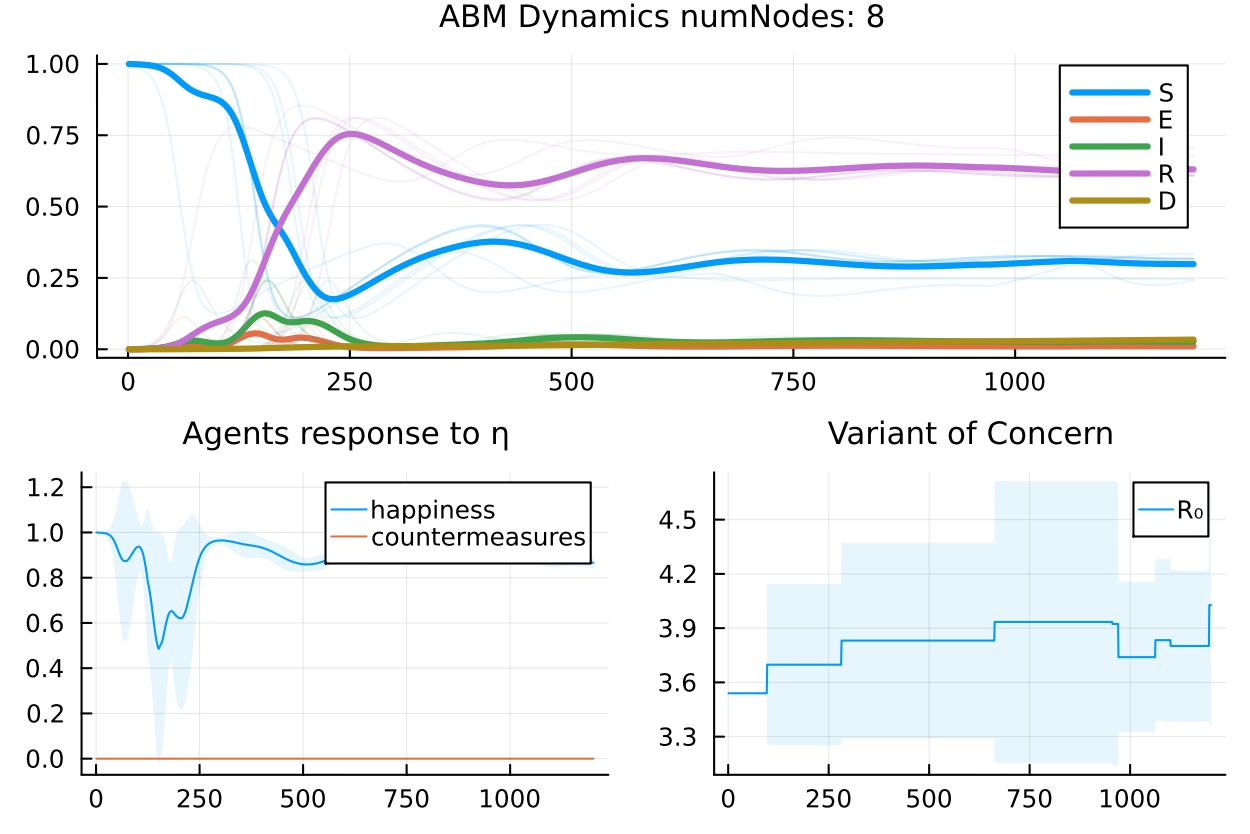
\includegraphics[width=\textwidth]{img/SocialNetworkABM_1_NN.jpg}
		\caption{Grafico per la comparazione sul numero di nodi della rete. Numero nodi 8}
		\label{fig:comparison_numberOfNodes_8}
	\end{subfigure}
	\hfill
	\begin{subfigure}[b]{0.45\textwidth}
		\centering
		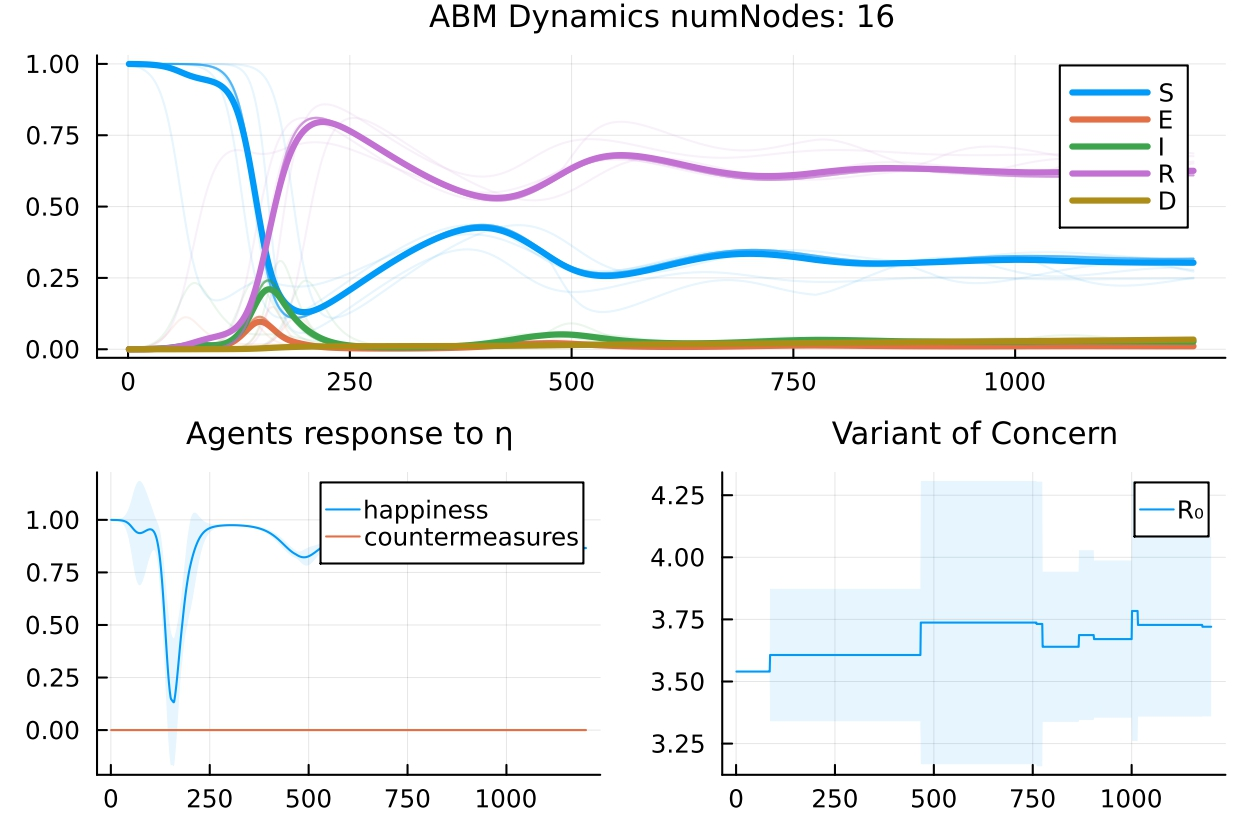
\includegraphics[width=\textwidth]{img/SocialNetworkABM_2_NN.jpg}
		\caption{Grafico per la comparazione sul numero di nodi della rete. Numero nodi 16}
		\label{fig:comparison_numberOfNodes_16}
	\end{subfigure}
	\hfill
	\begin{subfigure}[b]{0.45\textwidth}
		\centering
		\includegraphics[width=\textwidth]{img/SocialNetworkABM_3_NN.jpg}
		\caption{Grafico per la comparazione sul numero di nodi della rete. Numero nodi 32}
		\label{fig:comparison_numberOfNodes_32}
	\end{subfigure}
	\hfill
	\begin{subfigure}[b]{0.45\textwidth}
		\centering
		\includegraphics[width=\textwidth]{img/SocialNetworkABM_4_NN.jpg}
		\caption{Grafico per la comparazione sul numero di nodi della rete. Numero nodi 64}
		\label{fig:comparison_numberOfNodes_64}
	\end{subfigure}
\end{figure}

In sintesi, l'analisi ha dimostrato come il numero di nodi nella rete, 
insieme a variabili come la topologia delle connessioni e la posizione 
iniziale del focolaio, possa influenzare in modo significativo le 
dinamiche della pandemia e i profili temporali di infezione.

\subsection{Analisi del Comportamento in Base alla Copertura della Rete}

L'analisi condotta ha esaminato l'effetto della copertura della rete, 
rappresentata dal numero di archi, sul comportamento del modello. 
Dai risultati è emerso che una copertura bassa, ovvero un numero 
limitato di connessioni tra i nodi del grafo, ha comportato un 
rallentamento significativo nella diffusione del virus, analogamente 
all'effetto di misure di contenimento come il lockdown. 
Questo risultato è coerente con l'importanza della mobilità nella 
diffusione delle malattie infettive e sottolinea il ruolo cruciale 
delle misure di contenimento nel limitare la propagazione del virus.

Inoltre, è stato osservato che il numero di Varianti di Interesse 
(VOC) tende ad aumentare con il numero di nodi nella rete. 
Questo suggerisce che in una popolazione più ampia, c'è una maggiore 
probabilità di emergere nuove mutazioni. Tuttavia, è interessante 
notare che la presenza di una bassa copertura, cioè una limitata 
interconnessione tra i nodi, può limitare la diffusione delle varianti 
stesse, poiché la trasmissione tra gli individui è ridotta.

\begin{figure}[H]
	\centering
	\begin{subfigure}[b]{0.3\textwidth}
		\centering
		\includegraphics[width=\textwidth]{img/SocialNetworkABM_1_EC.jpg}
		\caption{Grafico per la comparazione sulla copertura della rete. Copertura alta}
		\label{fig:comparison_highCoverage}
	\end{subfigure}
	\hfill
	\begin{subfigure}[b]{0.3\textwidth}
		\centering
		\includegraphics[width=\textwidth]{img/SocialNetworkABM_2_EC.jpg}
		\caption{Grafico per la comparazione sulla copertura della rete. Copertura media}
		\label{fig:comparison_mediumCoverage}
	\end{subfigure}
	\hfill
	\begin{subfigure}[b]{0.3\textwidth}
		\centering
		\includegraphics[width=\textwidth]{img/SocialNetworkABM_3_EC.jpg}
		\caption{Grafico per la comparazione sulla copertura della rete. Copertura bassa}
		\label{fig:comparison_lowCoverage}
	\end{subfigure}
\end{figure}

In sintesi, l'analisi ha rivelato come vari parametri e condizioni, 
tra cui la copertura della rete, la mobilità, le misure di contenimento 
e il numero di nodi, possono influenzare in modo significativo il 
comportamento del modello epidemiologico. Questi risultati forniscono 
importanti informazioni per la comprensione e la gestione delle epidemie, 
evidenziando l'importanza delle strategie di mitigazione e della 
considerazione della struttura della rete nella prevenzione della 
diffusione del virus.
\newpage

\subsection{Studio dell'Andamento del Controllore in Relazione all'Intervallo di Intervento}
L'analisi condotta nel presente studio ha investigato l'influenza 
dell'intervallo di intervento del controllore in relazione al controllo 
della pandemia e all'andamento della curva di ``happiness''. I risultati 
ottenuti hanno rivelato che un incremento nel valore associato 
all'intervallo di intervento provoca un notevole sbilanciamento nella 
curva di felicità (``happiness'') e, in generale, comporta un repentino 
aumento nei valori associati alle contromisure adottate.

Tale andamento, coerente e previsto, può essere spiegato dalla 
complessità intrinseca nel formulare contromisure a lungo termine 
rispetto a quelle a breve termine, oltre al fatto che le prime 
comportano costi maggiori. È interessante notare che l'andamento delle 
curve, come mostrato nelle Figure \ref{fig:comparison_dt_21} e 
\ref{fig:comparison_dt_28}, ha rivelato comportamenti inaspettati che 
non erano stati previsti inizialmente. Questo comportamento inusuale è 
probabilmente riconducibile alla definizione della funzione di loss, 
come illustrato nella Figura \ref{fig:lossFunction}, e alle successive 
iterazioni di addestramento della rete.

In conclusione, dai risultati ottenuti emerge che attualmente le curve 
più affidabili sono quelle associate a un intervallo di intervento più 
breve. Tuttavia, è importante notare che non sono stati esplorati 
intervalli troppo granulari a causa del loro significativo impatto 
sulle prestazioni del sistema e, soprattutto, della loro limitata 
rappresentatività nella realtà.

\begin{figure}[H]
	\centering
	\begin{subfigure}[b]{0.45\textwidth}
		\centering
		\includegraphics[width=\textwidth]{img/SocialNetworkABM_1_DT.jpg}
		\caption{Grafico per la comparazione sul valore dell'intervallo di intervento del controllore. Valore 7 step}
		\label{fig:comparison_dt_7}
	\end{subfigure}
	\hfill
	\begin{subfigure}[b]{0.45\textwidth}
		\centering
		\includegraphics[width=\textwidth]{img/SocialNetworkABM_2_DT.jpg}
		\caption{Grafico per la comparazione sul valore dell'intervallo di intervento del controllore. Valore 14 step}
		\label{fig:comparison_dt_14}
	\end{subfigure}
	\hfill
	\begin{subfigure}[b]{0.45\textwidth}
		\centering
		\includegraphics[width=\textwidth]{img/SocialNetworkABM_3_DT.jpg}
		\caption{Grafico per la comparazione sul valore dell'intervallo di intervento del controllore. Valore 21 step}
		\label{fig:comparison_dt_21}
	\end{subfigure}
	\hfill
	\begin{subfigure}[b]{0.45\textwidth}
		\centering
		\includegraphics[width=\textwidth]{img/SocialNetworkABM_4_DT.jpg}
		\caption{Grafico per la comparazione sul valore dell'intervallo di intervento del controllore. Valore 28 step}
		\label{fig:comparison_dt_28}
	\end{subfigure}
\end{figure}

\subsection{Studio dell'Andamento del Controllore in Relazione all'Intervallo di Tolleranza}
L'analisi condotta nel corso di questa indagine ha approfondito 
l'influenza dell'intervallo di tolleranza del controllore in relazione 
al controllo della pandemia e all'andamento della curva di ``happiness''. 
Dalla nostra analisi emerge chiaramente che il valore di tolleranza del 
controllore svolge un ruolo cruciale soprattutto durante il picco pandemico.

Tuttavia, è degno di nota che un valore di tolleranza estremamente 
elevato incide in maniera significativa sull'andamento complessivo del 
modello, ritardando l'attuazione delle contromisure e costringendo il 
controllore ad adottare un comportamento molto più drastico rispetto alle 
aspettative.

È fondamentale sottolineare che tali risultati sono ampiamente 
condizionati dal numero di individui presenti in ciascun nodo del modello. 
Il test è stato condotto su un modello composto da cinquanta nodi, ognuno 
dei quali ospitava un numero di individui distribuiti secondo una 
distribuzione esponenziale con un parametro medio pari a 10.000. 
Questo implica che l'interpretazione dei risultati deve essere 
attentamente valutata tenendo conto del valore medio di popolazione 
all'interno del modello.

Evidentemente, è cruciale riconoscere come l'aumento del valore di 
popolazione generi risultati differenti. In scenari caratterizzati da 
valori di popolazione medio relativamente bassi, è possibile adottare 
una soglia di tolleranza più elevata, mentre in situazioni in cui la 
popolazione è notevolmente elevata, diventa necessario aumentare la 
tolleranza al fine di garantire un adeguato controllo.

In conclusione, l'analisi effettuata dimostra che l'intervallo di 
tolleranza del controllore rappresenta un fattore chiave nella gestione 
della pandemia e dell'andamento della ``happiness''. La sua ottimizzazione 
deve essere attentamente bilanciata in base al contesto specifico, inclusi 
il numero di individui e le dinamiche di popolazione, al fine di garantire 
un controllo efficace e tempestivo della pandemia.

\begin{figure}[H]
	\centering
	\begin{subfigure}[b]{0.45\textwidth}
		\centering
		\includegraphics[width=\textwidth]{img/SocialNetworkABM_1_TOL.jpg}
		\caption{Grafico per la comparazione sul valore di attivazione del controllore. Valore di tolleranza 0.0001}
		\label{fig:comparison_tol_1e-4}
	\end{subfigure}
	\hfill
	\begin{subfigure}[b]{0.45\textwidth}
		\centering
		\includegraphics[width=\textwidth]{img/SocialNetworkABM_2_TOL.jpg}
		\caption{Grafico per la comparazione sul valore di attivazione del controllore. Valore di tolleranza 0.001}
		\label{fig:comparison_tol_1e-3}
	\end{subfigure}
	\hfill
	\begin{subfigure}[b]{0.45\textwidth}
		\centering
		\includegraphics[width=\textwidth]{img/SocialNetworkABM_3_TOL.jpg}
		\caption{Grafico per la comparazione sul valore di attivazione del controllore. Valore di tolleranza 0.01}
		\label{fig:comparison_tol_1e-2}
	\end{subfigure}
	\hfill
	\begin{subfigure}[b]{0.45\textwidth}
		\centering
		\includegraphics[width=\textwidth]{img/SocialNetworkABM_4_TOL.jpg}
		\caption{Grafico per la comparazione sul valore di attivazione del controllore. Valore di tolleranza 0.1}
		\label{fig:comparison_tol_1e-1}
	\end{subfigure}
\end{figure}

In entrambi i contesti in cui sono stati esaminati e testati alcuni 
parametri fondamentali del controllore, è evidente come la curva di 
``happiness'' mostri un comportamento apparentemente opposto rispetto alla 
curva delle contromisure adottate. Questo fenomeno è chiaramente 
attribuibile alla natura estremamente semplicistica con cui è stata 
definita la curva di ``happiness'', come illustrato nella Figura 
\ref{fig:happinessf}.

Va notato che questa semplificazione nella rappresentazione della 
felicità è stata scelta consapevolmente per scopi specifici di questo 
studio, sebbene sia riconosciuta come irrealistica. Tuttavia, questa 
semplice rappresentazione ha dimostrato di essere adeguata per gli 
obiettivi attuali della ricerca. 

Nonostante l'apparente discrepanza tra i comportamenti delle due curve, 
è importante sottolineare che questa semplificazione sarà oggetto di 
ulteriori raffinamenti in futuro. Tale rifinitura mirerà a renderla più 
realistica e coerente con le dinamiche reali delle emozioni umane e 
delle reazioni della società a situazioni di emergenza.

In conclusione, la discrepanza osservata tra le curve di ``happiness'' e 
le curve delle contromisure è attribuibile alla semplificazione 
deliberata della curva di ``happiness'' utilizzata in questo studio. 
Tale semplificazione, sebbene irrealistica, è adeguata agli scopi attuali, 
ma verrà affinata in future ricerche al fine di migliorare la 
rappresentazione delle dinamiche umane in contesti pandemici e di 
emergenza.
\section{Risultati Ottenuti}

\subsection{Nessun intervento}
Il seguente grafico \ref{fig:abm_no_intervent} mostra l'andamento delle curve del modello
quando questo viene eseguito senza alcuna tipologia di intervento. Questo andamento e' mostrato 
in maniera cumulativa rispetto all'andamento dei singoli agenti, i quali possono mostrare comportamenti 
differenti tra loro.

\begin{minipage}{\linewidth}
	\centering
	\includegraphics[width=\textwidth]{img/SocialNetworkABM_NO_CONTROL.pdf}
	\captionof{figure}{Grafico cumulativo del modello senza senza alcun tipo di intervento}
	\label{fig:abm_no_intervent}
\end{minipage}

Complessivamente l'andamento del modello e' similare all'andamento standard di un modello di tipo  
SEIR, con qualche variazione dipendente dai fattori di stocasticita' intrisechi del modello; che in questo
caso non sono troppo presenti. Il grafico mostra le traiettorie piu' comuni delle curve cumulate del modello, 
dove vengono messe in evidenza i percorsi piu' utilizzati. 

Come e' possibile notare, il numero di individui suscettibili crolla drasticamente
per via della diffusione rapida e simil esponenziale che ha il virus. Questa viene emulata
dall'altrettanto rapida crescita di individui guariti (recovered) che pero', per via
di come e' stato definita la condizione di guariti, non sono immuni alle varianti del virus, permettendo 
di modellare una possibile ciclicita' dell'epidemia data dalla perdita di immunita' della popolazione. 
Queste proprieta' contribuiscono ad un andamento ciclico delle curve. Si puo' notare come 
la curva associata all'andamento degli individui nella classe \emph{D} abbia una crescita lineare, 
seppur non troppo evidente.

A seguire si puo' osservare come la curva associata alla variabile di happiness del modello,
valore che serve per bilanciare la durezza delle misure di controllo per evitare 
di cadere in un ciclo funzionale ma insostenibile, mostra un comportamento alquanto bizzarro.
Questo e' dovuto principalmente a come viene definita la funzione di controllo della felicita' \ref{fig:happinessf}.
Si osserva inoltre che la curva tende ad un \emph{plateau} passato il periodo della "prima ondata".

Questo comportamento principalmente irrealistico e associato alla definizione che e' stato fatto della 
funzione \textbf{happiness} \ref{fig:happinessf}. Il comportamento di questa curva non e' completamente 
realistico, ma e' comunque utilizzabile per lo scopo di mantenere sotto controllo le contromisure $\eta$.

\begin{minipage}{\linewidth}
	\centering
	\includegraphics[width=\textwidth]{img/coronavirus-data-explorer.png}
	\captionof{figure}{Grafico delle mutazioni del virus SARS-COV2 preso da Our World in Data}
	\label{fig:covid_mutation}
\end{minipage}

Infine si nota come, seppur la definizione della funzione associata alla creazione di una
nuova \emph{Variant of Concern (VOC)} \ref{fig:voc} sia semplicistica e irrealistica, 
il grafico mostra come su un periodo di circa 3 anni, associabile alla durata del periodo covid, 
il numero di VOC sia pressoche' sovrapponibile con quanto osservato dai dati raccolti durante la pandemia \ref{fig:covid_mutation}. 

\subsection{Intervento non farmaceutico}
Il seguente grafico \ref{fig:abm_intervent} mostra l'andamento delle curve del modello
quando questo viene eseguito tramite l'applicazione di una qualche tipologia di intervento non farmaceutico. 
Le contromisure sono rappresentate come un insieme di valori appartenenti all'intervallo $[0, 1)$ 
le quali rappresentano cumulativamente un insieme di metriche differenti non esplicite che vanno a definire 
un insieme di misure di controllo. Le misure di controllo cercano di mimicare quelle associate al progetto 
\textbf{OxCGRT} il quale ha lo scopo di misurare la durezza delle contomisure applicate in un determinato paese; 
questo valore e' composito di 9 metriche: chiusura delle scuole; chiusura dei luoghi di lavoro; 
cancellazione di eventi pubblici; restrizioni agli assembramenti pubblici; 
chiusura dei trasporti pubblici; obbligo di rimanere a casa; campagne di informazione pubblica; 
restrizioni agli spostamenti interni e controlli sui viaggi internazionali.

\begin{minipage}{\linewidth}
	\centering
	\includegraphics[width=\textwidth]{img/SocialNetworkABM_CONTROL.pdf}
	\captionof{figure}{Grafico cumulativo del modello con intervento non farmaceutico del controllore}
	\label{fig:abm_intervent}
\end{minipage}

Queste metriche sono metriche reali ma che nel modello vengono viste come un insieme unico, associabile 
ad una somma di medie dei valori di ogni metrica. Questa scelta porta a non avere un indice molto chiaro
ma permette comunque di avere un idea generale estremamente immediata dell'effetto che queste hanno sul modello.

Si nota come con l'applicazione di un insieme di contromisure, piu' o meno stringenti a seconda del periodo osservato, 
possiamo osservare come le curve epidemiologiche tendono ad appiattirsi, soprattutto quelle associate ai compartimenti 
\textbf{E, I}, le quali influenzano le curve \textbf{S, R}. In questo caso la ciclicita' del modello viene meno. 

Altro dato interessante e' il numero di VOC che e' diminuito rispetto al modello senza intervento.
Questo dipende generalmente dal comportamento delle contromisure. Infatti queste quando vengono applicate, 
oltre a influenzare il parametro \textbf{happiness}, vanno ad influenzare anche la matrice di flusso \ref{fig:migration matrix}
andando a ridurne i valori presenti. Questo fa si che oltre a dilazionare la diffusione della pandemia, 
va a dilazionare il comportamento della funzione che si occupa di generare una VOC \ref{fig:voc}. 

Questa infatti puo' attivarse sse nel nodo sono presenti individui infetti, in quanto non e' stata modellata la 
possibilita' che spontaneamente una nuova variante arrivi in un nuovo nodo senza un veicolo umano. Percio' 
applicare delle contromisure permette anche a contenere la diffusione di VOC nella popolazione osservata.

Si puo' osservare come la variabile di controllo \textbf{happiness} segua molto attentamente l'andamento sia delle 
contromisure che della pandemia, arrivando all'inizio della pandemia quando le contromisure sono piu' stringenti 
a diventare pressoche nulla. Successivamente, pur mantenendo un livello di contromisure sostenuto, la media
del valore di controllo tende ad alzarsi, seguendo il valore del compartimento \textbf{R}. Questo approccio sembra 
imitare il generale andamento della risposta che la popolazione italiana ha avuto alle prime misure di contenimento 
applicate realmente durante la pandemia da COVID-19.

\subsection{Intervento farmaceutico}
Il seguente grafico \ref{fig:abm_vaccine} mostra l'andamento delle curve del modello
quando questo viene eseguito tramite l'applicazione di una qualche tipologia di intervento farmaceutico.
Questo grafico dipende enormemente da quando viene trovato e successivamente applicato un intervento 
farmaceutico alla popolazione. Prima viene applicato un intervento farmaceutico piu' le curve si modificano 
e sono differenti dalll'andamento senza intervento \ref{fig:abm_no_intervent}, mentre piu' tempo passa piu'
il comportamento tende ad assomigliarsi.

\begin{minipage}{\linewidth}
	\centering
	\includegraphics[width=\textwidth]{img/SocialNetworkABM_VACCINE.pdf}
	\captionof{figure}{Grafico cumulativo del modello con intervento del controllore tramite interventi farmaceutici come ad esempio un vaccino}
	\label{fig:abm_vaccine}
\end{minipage}

Il grafico mostra come se disponibili e applicate repentinamente, l'utilizzo di contromisure farmaceutiche permette 
permette di ridurre repentinamente le curve senza andare ad intaccare la curva di happiness in maniera troppo sensibile.

\subsection{Intervento farmaceutico e non farmaceutico}
Il seguente grafico \ref{fig:abm_all} mostra l'andamento delle curve del modello
quando questo viene eseguito tramite l'applicazione sia di un intervento di tipo farmaceutico 
come ad esempio l'utillizo di un vaccino, che di contromisure non farmaceutiche.

\begin{minipage}{\linewidth}
	\centering
	\includegraphics[width=\textwidth]{img/SocialNetworkABM_ALL.pdf}
	\captionof{figure}{Grafico cumulativo del modello con intervento del controllore tramite vaccino e metodi di prevenzione non farmaceutici}
	\label{fig:abm_all}
\end{minipage}

In questo caso viene mostrato l'andamento delle curve tenendo in considerazione l'utilizzo di ogni mezzo
per prevenire e contrastare l'epidemia. L'uitilizzo combinato di mezzi farmaceutici e non permettono 
si appiattire notevolmente la curva di infetti andando a creare velocemente un immunita' di gruppo 
che rende la popolazione meno suscettibile alle varianti. Questo inoltre fa si che la \emph{happiness} media
del modello sia generalmente piu' alta anche quando vengono applicate delle contromisure che vanno ad 
intaccare la felicita' della popolazione (ad esempio un lockdown). 

Queste contromisure non farmaceutiche sono in genere meno stringenti e meno prolungate, permettendo quindi
alla popolazione di non avere un calo drastico della happiness generale come in figura \ref{fig:abm_intervent}.
Tuttavia dipendono fortemente da quando le contromisure farmaceutiche (il vaccino) vengono applicate
e con che efficacia questo riesce ad entrare in circolazione. 

Tuttavia questo dimostra come l'utilizzo di un vaccino a priori sia un metodo molto efficace per contrastare
una epidemia, e che ovviamente l'efficacia di questo dipenda molto e soprattutto da quando viene applicato 
alla popolazione. Successivamente si puo' notare come le misure non farmaceutiche di prevenzione e contrasto
dell'epidemia sono un mezzo efficace per controllare la diffusione dell'infezione, ma queste hanno un costo 
in termini sia di generale qualita' della vita, che anche economico, non indifferente come mostrato dai grafici 
precedenti e dall'esperienza diretta che si e' avuto con la pandemia da COVID-19. 

\subsection{Analisi di sensitività}
Osservando il modello SEIR definito come segue \ref{fig:ODE_Julia_example} 
si puo' osservare come quest'ultimo potrebbe essere sensibile al mutamento di specifici 
parametri al suo interno, i quali potrebbero portare il modello ad avere comportamenti 
peculiari e soprattutto imprevisti o inattesi.

Percio' e' stato deciso di effettuare un analisi di sensitivita' del sistema tramite l'utilizzo 
di metodi di libreria offerti dalla suite \emph{SciML.ai}. In questo modo e' stato possibile 
osservare a quali parametri il modello fosse piu' sensibile.

\begin{minipage}{\linewidth}
	\centering
	\includegraphics[width=\textwidth]{img/sa.pdf}
	\captionof{figure}{Grafico rappresentante l'analisi di sensitivita' del modello}
	\label{fig:sens_anal}
\end{minipage}

Come osservato in figura \ref{fig:sens_anal}, il modello ha una sensitivita' abbastanza 
uniforme per i parametri $R_0, \gamma$ e $\sigma$, il che era atteso in quanto sono tutti 
responsabili dell'avanzamento del contagio. La sensitivita' ai parametri $\omega$ e $\delta$ 
era comunque attesa, anche se non cosi' accentuata come mostrata in figura. Infine la sensitivita' 
relativa al parametro $\eta$ responsabile delle contromisure e' pressocche' inversa a quella del 
parametro $R_0$ il che e' relativamente atteso in quanto e' un parametro direttamente collegato 
alle contromisure per la diffusione del contagio. La sensitivita' al parametro $\xi$ invece ha 
andamento singolare e pare essere legato alla sensitivita' del parametro $\omega$ seppur in 
modo specchiato. Questo probabilmente perche' essendo i parametri $\omega$ e $\xi$ legati al 
compartimento \textbf{R} del modello, che gestisce gli individui sia guariti che vaccinati, 
il loro comportamento e' sensato che sia collegabile.

Successivamente e' stata applicato un controllo di sensitivita' riguardo i parametri 
relativi al modello ad agente in se, tramite l'utilizzo della funzione \textbf{paramscan} offerta
dalla libreria \textbf{Agents.jl}.

E' stato scelto un insieme di parametri del modello che vengono modificati all'interno di un range 
definito e in base alle varie configurazioni ottenute si va ad osservare come il comportamento del modello 
puo' o meno cambiare. I valori che sono stati scelti in quanto idealmente responsabili di un comportamento 
differente se modificati sono i seguenti: 

\begin{minipage}{\linewidth}
	\centering
	\includegraphics[width=\textwidth]{img/paramscan.png}
	\captionof{figure}{Parametri usati per l'analisi di sensitivita' del modello ad agente}
	\label{fig:paramscan}
\end{minipage}

Questi parametri sono stati scelti in come possibili parametri con un comportamento latente. I parametri 
relativi al controllore e al vaccino non sono stati inclusi per ovvi motivi, in quanto e' stato gia' dimostrato 
come il loro variare puo' portare a cambiamenti significativi all'interno della simulazione del modello 
\ref{fig:abm_no_intervent} \ref{fig:abm_intervent} \ref{fig:abm_vaccine} \ref{fig:abm_all}.

\newpage

In questo confronto si nota come il numero di nodi infetti iniziali influenzi principalmente la velocita' con cui 
il picco di infetti arriva a compimento. Si nota come nel caso in cui si inizi con un numero di nodi infetti maggiore, 
la curva degli infetti tendera' a essere prona verso l'inizio della linea temporale piuttosto che la fine, arrivando 
al proprio picco prima. Oltre a questo tuttavia non vi sono altri comportamenti degni di nota. Nel complesso e' un
comportamento atteso.

\begin{figure}[!hb]
	\centering
	\begin{subfigure}[b]{0.45\textwidth}
		\centering
		\includegraphics[width=\textwidth]{img/SocialNetworkABM_1.pdf}
		\caption{Grafico per la comparazione sul numero di nodi infetti di partenza. Numero nodi infetti iniziali 1}
		\label{fig:comparison_init_node_inf_1}
	\end{subfigure}
	\hfill
	\begin{subfigure}[b]{0.45\textwidth}
		\centering
		\includegraphics[width=\textwidth]{img/SocialNetworkABM_13.pdf}
		\caption{Grafico per la comparazione sul numero di nodi infetti di partenza. Numero nodi infetti iniziali 4}
		\label{fig:comparison_init_node_inf_4}
	\end{subfigure}
\end{figure}

Anche in questo caso si puo' osservare come la curva epidemiologica tenda a raggiungere un valore 
di picco piu' alto in un periodo di tempo minore nel caso in cui si ha un rateo di migrazione piu' alto. 
Anche questo comportamento era atteso e non sorprende.

\begin{figure}[!hb]
	\centering
	\begin{subfigure}[b]{0.45\textwidth}
		\centering
		\includegraphics[width=\textwidth]{img/SocialNetworkABM_1.pdf}
		\caption{Grafico per la comparazione sul valore di migrazione. Valore di 0.001}
		\label{fig:comparison_maxTravelingRate_low}
	\end{subfigure}
	\hfill
	\begin{subfigure}[b]{0.45\textwidth}
		\centering
		\includegraphics[width=\textwidth]{img/SocialNetworkABM_4.pdf}
		\caption{Grafico per la comparazione sul valore di migrazione. Valore di 0.01}
		\label{fig:comparison_maxTravelingRate_high}
	\end{subfigure}
\end{figure}

\newpage

In questo confronto e' lapalissiano come il numero di nodi della rete influenzi l'andamento delle curve epidemiologiche. 
I grafici mostrano come in genere un numero di nodi maggiore comporta ad una diffusione piu' lenta e con picchi meno ripidi
seppur piu' prolungati nel tempo. Ovviamente questo dipende da molteplici fattori, primo tra tutti la topologia delle connessioni 
del grafo e in secondo luogo dove il primo focolare ha inizio. 

\begin{figure}[!hb]
	\centering
	\begin{subfigure}[b]{0.45\textwidth}
		\centering
		\includegraphics[width=\textwidth]{img/SocialNetworkABM_1.pdf}
		\caption{Grafico per la comparazione sul numero di nodi della rete. Numero nodi 4}
		\label{fig:comparison_numberOfNodes_4}
	\end{subfigure}
	\hfill
	\begin{subfigure}[b]{0.45\textwidth}
		\centering
		\includegraphics[width=\textwidth]{img/SocialNetworkABM_17.pdf}
		\caption{Grafico per la comparazione sul numero di nodi della rete. Numero nodi 12}
		\label{fig:comparison_numberOfNodes_12}
	\end{subfigure}
	\hfill
	\begin{subfigure}[b]{0.45\textwidth}
		\centering
		\includegraphics[width=\textwidth]{img/SocialNetworkABM_33.pdf}
		\caption{Grafico per la comparazione sul numero di nodi della rete. Numero nodi 20}
		\label{fig:comparison_numberOfNodes_20}
	\end{subfigure}
	\hfill
	\begin{subfigure}[b]{0.45\textwidth}
		\centering
		\includegraphics[width=\textwidth]{img/SocialNetworkABM_49.pdf}
		\caption{Grafico per la comparazione sul numero di nodi della rete. Numero nodi 28}
		\label{fig:comparison_numberOfNodes_28}
	\end{subfigure}
	\hfill
	\begin{subfigure}[b]{0.45\textwidth}
		\centering
		\includegraphics[width=\textwidth]{img/SocialNetworkABM_65.pdf}
		\caption{Grafico per la comparazione sul numero di nodi della rete. Numero nodi 36}
		\label{fig:comparison_numberOfNodes_36}
	\end{subfigure}
\end{figure}

\newpage

In questa figura e' osservabile come la copertura della rete, data dal numero di archi che la compongono,
va ad influenzare in maniera sensibile l'andamento della pandemia, soprattutto nel caso in cui la copertura e' 
bassa \ref{fig:comparison_lowCoverage}. Tendenzialmente e' ipotizzabile che con una bassa copertura, quindi 
con una possibilita' piu' limitata di spostarsi da un nodo all'altro, la diffusione del virus subisce un arresto, 
e questo e' osservabile con i dati ottenuti durante la pandemia COVID-19 dove una della prime contromisure applicate 
e' stata quella del \textbf{lockdown generalizzato} in cui la capacita' di spostamento degli individui 
e' calata drasticamente.

\begin{figure}[!hb]
	\centering
	\begin{subfigure}[b]{0.3\textwidth}
		\centering
		\includegraphics[width=\textwidth]{img/SocialNetworkABM_65.pdf}
		\caption{Grafico per la comparazione sulla copertura della rete. Copertura bassa}
		\label{fig:comparison_highCoverage}
	\end{subfigure}
	\hfill
	\begin{subfigure}[b]{0.3\textwidth}
		\centering
		\includegraphics[width=\textwidth]{img/SocialNetworkABM_145.pdf}
		\caption{Grafico per la comparazione sulla copertura della rete. Copertura media}
		\label{fig:comparison_mediumCoverage}
	\end{subfigure}
	\hfill
	\begin{subfigure}[b]{0.3\textwidth}
		\centering
		\includegraphics[width=\textwidth]{img/SocialNetworkABM_225.pdf}
		\caption{Grafico per la comparazione sulla copertura della rete. Copertura alta}
		\label{fig:comparison_lowCoverage}
	\end{subfigure}
\end{figure}

E' accurato assumere come, dato il modo con cui viene creata la copertura degli archi, questa 
possa influenzare la diffusione del virus. In particolar modo la diffusione nel caso di alta e media copertura 
e' molto simile. Questo e' dovuto con molta probabilita' al modo in cui viene creata la copertura; modo che 
puo' essere osservato in figura \ref{fig:graph_coverage}

Cio' nonostante, quello che puo' essere ulteriormente osservato e' il comportamento sempre piu' "incerto" delle curve 
epidemiologiche al diminuire della copertura del grafo. Discorso similare si puo' osservare nella comparazione sul numero 
di nodi della rete, in cui le curve epidemiologiche tendono ad assumere un comportamento sempre piu' incerto all'aumentare dei 
nodi presenti in rete. Anche il numero di \textbf{VOC} pare aumentare con il numero di nodi, questo suggerisce che essendoci 
piu' individui la possibilita' di mutazioni aumenta, cosi' come diminuisce con il diminuire della copertura, stando ad indicare 
come seppur il numero di nodi possa essere elevato, ma se non vi e' una possibilita' o veicolo di infezione, le mutazioni difficilmente
possono accadere; diminuendo la pericolosita' dell'agente patogeno.

\begin{minipage}{\linewidth}
	\centering
	\includegraphics[width=\textwidth]{img/grpah_creation.png}
	\captionof{figure}{Esempio della funzione atta alla creazione di un grafo dato un determinato livello di copertura}
	\label{fig:graph_coverage}
\end{minipage}
\section{Sviluppi Futuri}
\subsection{Perfezionamento Controllore}
Uno sviluppo futuro può essere il perfezionamento del controllore sia nelle sue capacità di individuazione
e applicazione delle policy, sia nella chiarezza di ritornare delle policy \emph{human-understandable} così 
da essere facilmente tradotte e comprese anche da un operatore umano. Questo sviluppo apre le porte allo studio 
di causalità, elemento molto importante trattato in apertura dell'elaborato in quanto bisognerà cercare di capire 
una relazione che vi è tra l'applicazione di una specifica contromisura e il suo apporto alla diminuzione di una 
pandemia. 

Questo approccio è veramente complesso ma di estremo interesse in quanto potrebbe risultare in un balzo 
tecnologico non indifferente. 

\subsection{Miglioramento funzione happiness}
Un'altro grande scoglio definito come assunzione è la funzione di happiness, responsabile del 
controllo della funzione Controllore. Questa funzione attualmente serve solamente come brutale asticella per evitare 
di cadere all'interno di un ciclo disfunzionale di contromisure insostenibili nella vita reale. Tuttavia 
se venisse migliorato tenendo conto di quanto veramente ogni topologia di contromisura possa impattare sulla vita 
delle persone, sia sul breve che sul lungo periodo, questo potrebbe essere una pietra miliare per l'accuratezza delle 
policy sviluppate in quanto si avrebbe un valore di riscontro molto più accurato. 

Tuttavia anche questa sezione richiede un attenta analisi della causalità degli eventi, in particolare stimare quanto in 
generale una contromisura possa impattare l'umore di una popolazione. Umore il quale varia in maniera sia per via delle contromisure 
che anche per stimoli esterni alle volte neanche immaginabili. Ad aiuto sarebbe comodo avere a corredo molteplici \emph{benchtest} caratterizzati 
da differenti modelli di simulazione; partendo da quello più granulare per comprendere il comportamento emergente relativo 
al livello generale di soddisfazione di una popolazione dato un ambiente dinamico e auto influenzante, fino ad arrivare a mettere 
tutto quanto ottenuto insieme per avere una simulazione macroscopica in grado di offrire risultati affidabili.

\subsection{Perfezionamento generale modello}
Il modello implementato si basa su una serie di assunzioni relativamente ragionevoli, date dall'osservazione empirica
di quanto si voleva andare a modellare. L'osservazione e i dati raccolti durante tutto il periodo COVID-19 sono stati 
utili per ottenere un modello che possa essere abbastanza veritiero. Ciò nonostante questo modello attualmente non si presta
molto bene alla generalizzazione, ponendo il fianco a delle rigidità strutturali che ne compromettono l'uso. 

è quindi buona pratica quella di avere un modello che ben si adatti e generalizzi ai vari problemi cui viene sottoposto.

\subsection{Ottimizzazione generale}
Il codice sviluppato sicuramente ha nampio margine di miglioramento soprattutto sotto l'aspetto delle performance generali. 
In futuro è un nobile obiettivo quello di renderlo più efficiente, scalabile e ottimizzato possibile.



\nocite{*}
\bibliographystyle{IEEEtran}
\bibliography{reference.bib}

\appendix
\section{Altri Approcci}

\subsection{Modello ad Agente su Spazio Continuo}

L'approccio iniziale prevedeva la modellazione di una popolazione 
attraverso l'utilizzo di uno spazio di modello continuo. 
Gli agenti sarebbero stati rappresentati come individui reali, 
con un'effettiva presenza all'interno dello spazio. Questo spazio 
di modello continuo poteva essere visualizzato come una griglia di 
dimensioni $N \times M$ in cui gli agenti venivano posizionati in 
modo casuale e rappresentati come punti colorati.

\begin{figure}[H]
	\begin{center}
		\includegraphics[width=\textwidth]{img/ball-covid.png}
        \caption{Esempio del modello modellato su spazio continuo}
		\label{fig:ball_covid}
    \end{center}
\end{figure}

Questo approccio prendeva spunto dalla fisica delle palline da 
biliardo per modellare le interazioni tra gli agenti all'interno 
dello spazio del modello. Ogni agente poteva casualmente infettare 
un vicino solo se interagivano, e questa interazione veniva modellata 
come un urto elastico tra corpi, anche se non rappresentava un vero 
simulatore di urti elastici, bensì ne prendeva spunto.

Tuttavia, questo approccio è risultato eccessivamente granulare e 
poco adatto agli obiettivi del progetto. Inoltre, richiedeva una 
quantità considerevole di risorse computazionali e tempo, il che 
ha portato alla sua sostituzione con un approccio più astratto e flessibile.

\begin{figure}[H]
	\begin{center}
		\includegraphics[width=\textwidth]{img/plot_abm_continuousspace.jpg}
        \caption{Esempio del comportamento delle curve nel modello continuo}
		\label{fig:seir_curve_continuous}
    \end{center}
\end{figure}

\newpage

\subsection{Modello ad Agente con Spazio a Grafo e Modellazione Singolo Agente}

Un secondo approccio è stato progettato per consentire un maggiore 
controllo sullo spazio di modello e la sua evoluzione locale, 
piuttosto che sugli agenti individuali. Tuttavia, questo approccio 
ha incontrato problemi significativi, tra cui tempi di esecuzione 
estremamente lunghi e un comportamento delle curve epidemiologiche 
completamente divergente rispetto al modello SEIR deterministico. 
Questo comportamento anomalo è stato osservato in presenza di variazioni 
nel parametro $R_0$, e la causa rimane sconosciuta.

\begin{figure}[H]
    \begin{center}
		\includegraphics[width=\textwidth]{img/COMPARISON DIFFERENT R0 VALUE_2023-06-29.jpg}
		\caption{Comportamento modello ABM su spazio a grafo al variare del parametro $R_0$}
		\label{fig:strange_behaviour_R0_abm}
	\end{center}
\end{figure}

\begin{figure}[H]
    \begin{center}
		\includegraphics[width=\textwidth]{img/COMPARISON DIFFERENT R0 VALUE_2023-06-29 (1).jpg}
		\caption{Comportamento modello SEIR al variare del parametro $R_0$}
		\label{fig:strange_behaviour_R0_ode}
	\end{center}
\end{figure}

Anche se è stata formulata una formula approssimativa per 
descrivere la relazione tra i risultati del modello ABM e SEIR, 
questo comportamento rimane inspiegabile. 

$$ ADAPTED R_0 = 1.1730158534328545 + 0.21570538523224972 * x $$

L'uso di un approccio basato su un grafo e la modellazione del 
singolo agente ha portato a risultati incoerenti e ha reso necessario 
abbandonare questa metodologia a favore di alternative più promettenti.
\newpage

\subsection{Controllore Ipopt}

È stato esplorato un terzo approccio basato su Ipopt 
(Interior Point OPTimizer), un pacchetto software per l'ottimizzazione 
non lineare su larga scala. Ipopt è progettato per trovare soluzioni 
locali a problemi di ottimizzazione matematica, con funzioni obiettivo e 
vincoli non lineari. \cite{Wächter2006}

\begin{figure}[H]
	\begin{center}
		\includegraphics[width=\textwidth]{img/Comparison-of-Ipopt-performance-over-various-linear-solvers-using-the-two-dimensional.png}
		\caption{Comparison of Ipopt performance over various linear solvers using the two-dimensional partial differential equation test problem set. \cite{tasseff2019exploring}}
		\label{fig:Ipopt_solver}	
    \end{center}
\end{figure}

L'approccio ha previsto l'applicazione di un sistema di 
monitoraggio e intervento all'interno del modello di simulazione, 
con l'obiettivo di ridurre il numero di individui infetti. 
Le regole per il comportamento del modello sono state definite, 
inclusa una rappresentazione degli stati SEIR e un nuovo stato per 
il controllo delle risorse.

\begin{figure}[H]
	\begin{center}
		\includegraphics[width=\textwidth]{img/controller_ipopt.png}
		\caption{Definizione del controllore tramite la suite \texttt{Ipopt}}
		\label{fig:controller_ipopt}	
    \end{center}
\end{figure}

\begin{figure}[H]
	\begin{center}
		\includegraphics[width=\textwidth]{img/controller_rules.png}
		\caption{Definizione esplicita delle regole da applicare per la fase di ottimizzazione del modello da parte del controllore}
		\label{fig:controller_rules}	
    \end{center}
\end{figure}

\begin{figure}[H]
	\begin{center}
		\includegraphics[width=\textwidth]{img/controller_rules_1.png}
		\caption{Definizione esplicita delle regole da applicare per la fase di ottimizzazione del modello da parte del controllore per le contromisure}
		\label{fig:controller_rules_1}	
    \end{center}
\end{figure}

Sono state stabilite anche regole per il consumo di risorse, 
rappresentando le contromisure con il loro costo associato. 
L'ottimizzazione del modello è stata eseguita e sono stati restituiti 
i valori medi delle contromisure applicate.

I risultati ottenuti con Ipopt sono stati confrontati con quelli 
dell'implementazione personalizzata, rivelando somiglianze 
significative. Tuttavia, la possibilità di convertire facilmente 
il codice da CPU a GPU è stata determinante nella decisione di 
utilizzare l'implementazione personalizzata, in previsione di futuri 
miglioramenti delle prestazioni del codice.

\begin{figure}[H]
	\centering
	\begin{subfigure}[b]{\textwidth}
		\centering
		\includegraphics[width=\textwidth]{img/SocialNetworkABM_IPOPT_CONTROL.jpg}
		\caption{Risultato applicazione controllore tramite la suite Ipopt}
		\label{fig:ipopt_res1}
	\end{subfigure}
	\hfill
	\begin{subfigure}[b]{\textwidth}
		\centering
		\includegraphics[width=\textwidth]{img/SocialNetworkABM_IPOPT_ALL.jpg}
		\caption{Risultato applicazione controllore tramite la suite Ipopt}
		\label{fig:ipopt_res2}
	\end{subfigure}
\end{figure}

L'approccio ibrido del controllore è stato preferito per la sua 
semplicità e la possibilità di mascherare la funzione obiettivo 
tramite una rete neurale, semplificando notevolmente la definizione 
delle regole rispetto all'implementazione esplicita di Ipopt.

\end{document}